\documentclass[a4paper,12pt,twoside]{book}
\usepackage[utf8]{inputenc}
\usepackage[english]{babel}
%\usepackage{fontspec}
%\setmainfont[
%  Ligatures=TeX,
%  Extension=.otf,
%  BoldFont=cmunbx,
%  ItalicFont=cmunti,
%  BoldItalicFont=cmunbi,
%  SlantedFont=cmunsl
%]{cmunrm}

%\usepackage{polyglossia}
%\setmainlanguage{spanish}

\usepackage[c5paper]{geometry}
%\geometry{inner=2.5cm,outer=2.5cm,bmargin=3.2cm}
%\usepackage[DIV=14,BCOR=2mm,headinclude=true,footinclude=false]{typearea}

%\usepackage{ulem} %Hace que \emph sea subrayar

%\usepackage[p,osf]{scholax}
%% T1 and textcomp are loaded by package. Change that here, if you want
%% load sans and typewriter packages here, if needed

\usepackage{ebgaramond}
%\usepackage[type1]{libertine} % Linux Libertine for zweispaltige Texte
%\usepackage{textcomp}% Required to get special symbols
\usepackage[scaled=.8]{DejaVuSansMono}% FiraMono Typewriter font
\usepackage{PTSansNarrow} 
%\gilliuscondensed
%\usepackage[sfdefault]{FiraSans}
%\usepackage{bm}% Extra bold faces
%\usepackage[lf]{carlito}

\usepackage{lettrine} %Capital letters at the beginning of a chapter
\usepackage[activate={true,nocompatibility},final,tracking=true,kerning=true,spacing=true,factor=1100,stretch=10,shrink=10]{microtype}
\SetTracking{encoding={*}, shape=sc}{-20} % versalitas menos separadas
% activate={true,nocompatibility} - activate protrusion and expansion
% final - enable microtype; use "draft" to disable
% tracking=true, kerning=true, spacing=true - activate these techniques
% factor=1100 - add 10% to the protrusion amount (default is 1000)
% stretch=10, shrink=10 - reduce stretchability/shrinkability (default is 20/20)

%\usepackage{array,multirow,booktabs,colortbl,chngcntr} % El último es para counterwithout;
\usepackage[strict]{changepage}
%\usepackage{caption}
%\captionsetup{format=plain,labelsep=newline,labelfont={small,sc},
%textfont={small,it},singlelinecheck=false}
\usepackage[Bjornstrup]{fncychap} % Para cabeceras de capítulos sofisticados:     Sonny,    Lenny,    Glenn,    Conny,    Rejne,    and Bjarne.

\usepackage{graphicx,wrapfig,booktabs,multicol} % wallpaper: poner imágenes de fondo; wrapfigure: figuras a un lado del texto
%\graphicspath{{figures/}}
\usepackage{fancyhdr}
\usepackage{emptypage,pdfpages,fancybox} % Para que las páginas en blanco no tengan encabezado;
\usepackage{enumitem} %paralist: para compactenum, enumerate sin espacios
%\setlist[itemize]{nosep} %Espacio entre items en itemize
\usepackage[hyperref]{xcolor}
\usepackage[hidelinks]{hyperref}
\usepackage{xurl}

%\usepackage{minipage}

%\usepackage{quotchap} %Encabezados de capítulos
\usepackage{syntonly,verbatim}
%\syntaxonly

\usepackage{setspace,xspace} % xspace: Da \xspace para no tener que poner {} después de los comandos; pdflscape: páginas en horizontal;

\newenvironment{quotex}{\begin{quote}\small}{\end{quote}}
\newenvironment{quotationx}{\begin{quotation}\small}{\end{quotation}}


\begin{document}

% Por alguna razón, los marginados se creaban al revés. Así los corrijo. Feo, pero eficaz:
\let\tmp\oddsidemargin
\let\oddsidemargin\evensidemargin
\let\evensidemargin\tmp
\reversemarginpar

%\setcounter{secnumdepth}{4} % Para que llegue a numerar hasta las subsubsecciones;
%\renewcommand{\heavyrulewidth}{0.14em} % Grosor de las líneas extremas de las tablas;
%\renewcommand\thempfootnote{\alpha{mpfootnote}} % Símbolo de notas dentro de minipage
%\let\oldcaptionof\captionof
%\renewcommand{\captionof}[2]{\oldcaptionof{#1}{\newline \textit{#2} }}
%\renewcommand{\tablename}{Tabla}
%\counterwithout{figure}{chapter}
%\counterwithout{table}{chapter} % Así la numeración es 1, 2, 3... y no 1.1, 1.2... y no reinicia la num. en cada capítulo;

%\providecommand{\ggl}{\guillemotleft}
%\providecommand{\ggr}{\guillemotright\xspace}
\providecommand{\flright}[1]{\begin{flushright}#1\end{flushright}}
\providecommand{\flrightit}[1]{\begin{flushright}\itshape #1\end{flushright}}
%\renewcommand\UrlFont\sffamily
\urlstyle{tt}

\pagestyle{fancy}
\renewcommand{\sectionmark}[1]{\markright{#1}}
\renewcommand{\chaptermark}[1]{\markboth{#1}{}}

%Portada:
%\includepdf{00Portada}

\frontmatter
%
%\onehalfspacing
%\pagenumbering{Roman} %gobble es como empty

%\include{preindice}

%\fancyhf{}
%\fancyhead[LE]{\small \textbf{\thepage}$\quad$ Índice general}
%\fancyhead[RO]{\small Índice general $\quad$\textbf{\thepage}}
%\clearpage
\tableofcontents

%\doublespacing
\mainmatter

\fancyhf{}
\fancyhead[LE]{\small \thepage$\quad${\scshape\chaptername{} \thechapter}: \nouppercase{\itshape\leftmark}}
\fancyhead[RO]{\small \textsc{Section }\thesection{}: \nouppercase{\itshape\rightmark} $\quad$\upshape\thepage}
%\cfoot{\bfseries\thepage}

\pagenumbering{arabic}

%\onehalfspacing

% introductorios

\chapter{Introduction}
\section{Philosophic Idealism}

It is easy to be unaware that up until World War II, idealism was the dominant philosophical position of Europe. In the
18th and 19th century, the Germans — particularly Kant, Hegel, Fichte, Schelling, Schopenhauer — took the leading role in its development. Later, the Britons such as Green, Bradley, Bosanquet, Collingwood took it in
their own direction. In France, it usually went by the name of personalism or spiritualism. In Italy, while Evola was a
young man, philosophy was dominated by the idealists Benedetto Croce and Giovanni Gentile. It’s hard to
believe that at their peak, they were world-renowned philosophers. Although friends and collaborators, they split over
the question of Fascism. Gentile was for a while the education minister and his philosophical system was very
influential in moulding the intellectual roots of Fascism.

Yet idealism was not a modern development; the mainstream of Western philosophy is the history of idealistic thought.
When the European orientalists began studying, translating, and cataloguing the early Indo-Europeans systems of the
Vedas, its compatibility with idealism was noted. So, idealism can rightly be seen as “our” tradition and competitors
such as nominalism, positivism, and materialism are more like a persistent anti-tradition. I would recommend the short
book \textit{Nobilitas} by Alexander Jacob for a summary of this tradition from Plato until World War II. Ironically, Prof.
Jacob is an Indian who is keeping the Western philosophical tradition alive, when Europeans are abandoning it.

Evola was heir to this tradition and his intellectual development took place in the milieu of Italian idealism in the
1920s. In order to study idealism thoroughly, Evola learned German so he could read the philosophical sources in their
original language. Out of his studies, he created his own system which he named “magical idealism”. In The Individual
and the Becoming of the World, Evola ties together the main elements of his system. One can perhaps recognize
Schopenhauer when Evola speaks of in the world as will and representation, or Stirner in the idea of the Absolute Ego,
and Plotinus in the idea of privation and the evil of matter.

But Evola was not content in outlining an abstract intellectual system. Ultimately, there can be no system per se, since
what is important is the will and the development of its freedom to create, remake, and define the world. This means
that without having made the effort at self-transformation through the various phases of consciousness, then his system
cannot be properly comprehended. So ultimately, Evola’s system cannot be reduced to a set of propositions
to learn and memorize. Nor is there any technique, drug, or practice that will develop the will and lead to higher
stages of consciousness.

In our day, when “tough minded” thinkers are drawn to science and materialism (the neo-Darwinist Richard Dawkins was
recently “voted” the most intelligent man in Britain), the claims of idealism can seem incredible. Since Evola simply
assumes a basic familiarity with this tradition, it may be difficult sometimes to see what he is getting at. For those
new to idealism, I would recommend The Philosophy of Schopenhauer by Bryan Magee for a clear overview of the
presuppositions and methods of idealism. Whether or not Evola adds to this tradition in a coherent and constructive way
is for each man — who has made the requisite effort — to decide.

\flright{\itshape Posted on 2008-06-08 by Cologero}

\section{The Philosophy of the Future}

\begin{quotex}
The heart has its reasons that reason does not know. \flright{\textsc{Blaise Pascal}}
\end{quotex}

\paragraph{Evola and Gentile}
During \textbf{Julius Evola}'s youth, \textbf{Giovanni Gentile} was the grey eminence of philosophy in
Italy, not just in a university setting, but also close to the seat of political power. He was the epitome of the
cultured European, incorporating the whole of philosophy, art, literature, and history into his comprehensive system,
which he named “actualism”. So Evola's attack on Gentile was an attack on the Italian political,
intellectual, and educational edifice. Gentile never responded personally to Evola's critique, but instead
allowed his student \textbf{Ugo Spirito} to address the issues raised by Evola. But the first issue to consider is the
fundamental aim of philosophy, and this is where the two minds differ. Gentile's first political post was
the Minister of Education, which he used to reform the Italian school system. Evola's goal was much higher:

\begin{quotex}
If Gentile could truly name the I as the “pure act” of his rationalism, then he would appear not as the university
professor, whose “actualism” has the reform of the educational system as its goal, but rather as that cosmic centrality
that the esoteric reveals in the types of the rishi, the yogi, Christ, and the Buddha. 

\end{quotex}

So Evola's real objection is that Gentile sells himself short; the I, in its self-actualization, should have
as its goal to become a rishi, yogi, Christ, or Buddha. This, then, is the logical development of actualism that
Gentile somehow missed. While Evola's system has some defects, the goal is worthy.

To describe that goal, Evola has to incorporate elements of Oriental thought, for example, if Atman is Brahman, then how
does that affect philosophy? The influence of Friedrich Nietzsche is also strong, since it is now impossible to be a
philosopher without dealing with his withering critique of the decadence of Western thought and spirituality. This we
will address in the next section.

Ultimately, Evola never developed the philosophy of magical idealism, certainly not to the point of developing more
Christs and Buddhas. Even during the fifties and sixties, when allegedly there was a stream of young men who consulted
with him, no one arose to carry on that philosophy. By then, I suppose, idealism was a non-starter as the basis for a
philosophical system, and people were looking for less abstractions, turning instead to political and religious
solutions to the problems posed.

Evola himself, having first promoted a philosophy of action, resorted to passivity as in the aristocrat of the soul and
riding the tiger. Of course, while every Tom, Dick, and Harry nowadays claim to be an aristocrat of the soul, the
rishis are still hard to find.

\paragraph{The Philosopher of the Future}
If magical idealism is not the philosophy of the future, then we are still waiting for the philosopher of the future.
Those with a sound intellect should aspire to this, and not be content with the comfortable life of writing clever and
erudite journal papers. Aside from Kant, the great philosophers developed their view of life in their twenties. So
start now, you can always revise it.

Now there are three claimants to the knowledge of ultimate reality: the \emph{Priest}, the \emph{Philosopher}, and the
\emph{Prophet}. Borrowing an insight from \textbf{Valentin Tomberg}, we can say that the philosopher works in the day
through the light of reason, the prophet in the night through direct illumination from God, and the priest is the
mediator between the light and the darkness. The philosopher of the future will probably be in tension with the other
types, while still needing to incorporate their insights.

The philosopher must first deal with facts, then an understanding of the facts, and finally indicate how that affects
our lives. The fundamental facts have been summarized by \textbf{Arthur Schopenhauer}: the world as will and idea. Here
we find the Traditional doctrine of the two worlds of being and becoming. The “world” referred to is that of becoming,
and the “idea” is the world of being. Here are some examples.

\textbf{Plato}, and the lineage following him, called the will “eros”, i.e., the drive or “love” of wisdom. Wisdom, for
him, is to know the world of being. For Nietzsche, this overvaluing of the “other” world in Plato and in the
Christianity which built on Platonic ideas, led man away from his true calling of being fully loyal to the earth. There
is no other worldly afterlife beyond this world, but only its endless repetition. The Will to Power replaced eros. In
denying the world of being, Nietzsche denies God, or better, God, for him, is yet to come.

As a Traditional thinker, Evola opposed Nietzsche's biologism, while incorporating his more important
insights. While not denying the world of being, he changed man's relationship to it. First of all, he
retained Nietzsche's emphasis on will and action; this, as we have seen, brought him into conflict with
Rene Guenon. Now action can be understood in two ways. The conventional way is to see it as “horizontal”, i.e., as
activity wholly in the world of becoming. A deeper way is to understand it “vertically”, i.e., as the actualization of
potentialities. In this way, Evola can claim that it is insufficient to \emph{know the truth}, one must also \emph{will
the truth}. This implies absolute freedom.

The philosopher of the future can build on this. A rishi, or a seer, is more like a prophet than a philosopher. Hence,
he must learn to think with his heart as well as with his head. If the goal of philosophy is to bring God's
presence into the world, then he must learn to do that himself. To be free means to have no sufficient reason outside
oneself, so the philosopher must be free. Since for God, essence and existence coincide. Hence, the philosopher of the
future must actualize all his possibilities. Now we mean the philosopher is God-like in the relative, not the absolute
sense. How that is so, will be the task of this philosopher to explain.

\paragraph{The Religion of the Future}
The religion of the future will be based on gnosis. This is not a new religion, but rather a deeper understanding of
what religion is and means. In other words, it is the actualization of religious or spiritual understanding. This is
reflected in various states of consciousness, both psychological and spiritual. I am not making this up and have amply
documented how this has always been the case.

There are two false claimants to the religion of the future: one is to alter it to bring it into conformism with
modernity, the other is to repeat the religious forms of the past. Now there is no problem with the second option for
those who are satisfied with it. But the prophet of the future will write a large book on the phenomenology of the
soul.

\paragraph{2018 Postscript}
In a recently published collection of letters between \textbf{Wolfgang Smith} and Fr. \textbf{Malachi Martin}, there is
this intriguing comment from Prof. Smith:

\begin{quotex}
If the Greek Fathers could integrate Plato and Neoplatonism into the Christian worldview, and St. Thomas Aquinas could
do the same for Aristotle, why should it not be possible, in our day, to correct and somehow “Christianize” Hegel, let
us say, or Schelling, or even Nietzsche? Is there not in each of these German “Titans” a certain spark of truth that
needs to be brought out, to be “liberated”? 

\end{quotex}
That would be a good task for a young scholar. The starting point, of course, would be \textbf{Jacob Boehme}, the father
of German Idealism. Also, \textbf{Vladimir Solovyov}, who has already adapted Schelling into his system.

\flright{\itshape Posted on 2014-06-26 by Cologero}

\begin{center}* * *\end{center}

\begin{footnotesize}\begin{sffamily}

\texttt{seeker on 2014-06-26 at 13:25 said: }

You bring to mind Fr. Seraphim Rose's book (Orthodoxy and the Religion of the Future)? He gave the term a
decidedly pejorative connotation, referring specifically to New Age syncretism, one of the false claimants, “bringing
it into conformism with modernity”. But he was also critical of Hinduism, saying that the yogis experience during
meditation are mere psychic phenomena and not real spiritual knowledge.

The book was obviously not meant for the “rishi, yogi, Christ, or Buddha”. In this letter he refers to the Kali Yuga by
name, which leads me to believe there is more to his thought than one would gather from the above mentioned book. 

\hfill

\texttt{Ash on 2014-06-27 at 00:31 said: }

Concerning the relationship of the philosopher to gnosis: would such a person have already attained such a high state of
existence themselves? Or would they be showing the way as travelers themselves? I suppose two tests for such a
philosopher would be a) are they practicing a living exoteric tradition, and b) are they old enough to have gained
wisdom over time. So anyone starting now in their twenties ought to be preparing themselves for that.

\hfill

\texttt{Cologero on 2014-06-27 at 00:44 said: }

Seeker, I have not read that particular book, but I had previously read the letter you linked to. Obviously, I am being
a bit tongue in cheek and am not advocating anything like New Age … actually quite the opposite if read carefully.
Don't forget that Fr Rose also warned against “super-correctness”\footnote{\url{http://orthodoxinfo.com/ecumenism/fsr_63.aspx}}, and we have been criticized many times
by the super-correct. The problem today is one of a worldview. There was an earlier time when men could think with
their heart and were acutely aware of the reality of the other world of being. But now, such a mentality is utterly
alien to most men, so an intellectual conversion of some sort is necessary. So the way forward is actually a recovery,
but at a deeper level. That is because a man who has had to work for something appreciates it more than the man for
whom it came without effort.

I have been planning a post on the mental and spiritual states of the yogis, but much preparation is required.
Ultimately, it will be up to the prophet of the future to make such distinctions. Now Fr Rose was totally into Guenon
before he was not, so it is legitimate to speak to the former class of men as well as to the post-Guenon men. Careful
readers will need to sort it out.

\hfill

\texttt{Cologero on 2014-06-27 at 07:45 said: }

As I pointed out, Ash, most great philosophers developed their philosophy in their youth … I suppose we can find
examples and counter-examples. But the philosopher is a just “lover of wisdom” and so is not necessarily “wise”. There
are ultimate facts and the philosopher tries to understand them in the light of his own reason. The best are not
daunted by the complexity and enigmas of reality. In our time, there are new forms of escapism, even more insidious
that the decadent Christianity that Nietzsche or Evola opposed.

These forms of escapism are obvious enough to name. First are the so-called “new atheists”, who believe science and a
narrowly conceived rationality can account for all of reality. The other is new age political correctness which through
shaming and self-deception tries to enforce a worldview involving beliefs that no well-bred and healthy-minded man
could have believed in previous eras.

So, this imaginary philosopher would have to challenge those forms of escapism and describe a worldview in which the
quest for gnosis “makes sense”. So, yes, a man in his twenties ought to be preparing for that, “as if”, before his mind
stagnates.

\hfill
\end{sffamily}\end{footnotesize}
\section{The God of the Metaphysicians}

\begin{quotationx}
Even as regards those truths about God which human reason could have discovered, it was necessary that man should be
taught by a divine revelation; because the truth about God such as reason could discover, would only be known by a few,
and that after a long time, and with the admixture of many errors.  \flright{\emph{Summa Theologiae}, I.1.1}

Any “dualism”, whether of the theological order like that attributed to the Manicheans, or of the philosophical order
like that of Descartes, is a radically false conception. \flright{\textsc{Rene Guenon}}

\end{quotationx}

\begin{wrapfigure}{tr}{.35\textwidth}
 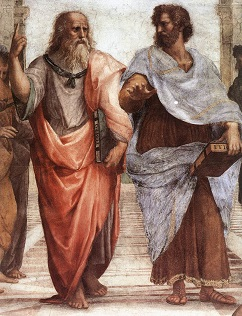
\includegraphics[scale=2.1]{a20151103TheGodofTheMetaphysicians-img001.jpg} 
\end{wrapfigure}

It is said that St Jerome was severely chastised for preferring to read the pagan philosophers rather than Sacred
Scriptures\footnote{\url{http://catholicharboroffaithandmorals.com/St.\%20Jerome.html}}. So it is with some caution that I turn to the pagans, not to commend them, but rather because such writings
have been a great part of my own personal equation. In particular, I am interested in those systems that assume the
intelligibility of the world through thought. These have been known as “Absolute Idealism” or “Monism”. We prefer the
first term, not always used in the strict sense; moreover, they have more of a “family resemblance” and not a totally
common teaching. In short, it represents the Platonic thread in philosophy rather than the Aristotelean. \textbf{Joseph
Marechal}, in \emph{Studies of the Psychology of the Mystics}, compares it to a strict monotheism as the foundation of
a certain type of mysticism.

It is easy to forget that up until a century again, it comprised what was properly called philosophy for educated men.
Other systems of thought, e.g., materialism, naturalism, etc., are not really philosophies since they deny the primacy
of thought. From Plato and Plotinus, it was revived with the German thinkers. The British then adapted their own
version, e.g., with T H Green, Francis Bradley, Bosanquet, etc. A century ago, it was dominated by the Italians
Benedetto Croce and Giovanni Gentile. Julius Evola, who learned German in order to study the German idealists, was also
an Absolute Idealist. Even Rene Guenon, although he disdained profane philosophy, had points in common with such
systems.

The neglect of Absolute Idealism has allowed inferior ideologies to take hold among the educated classes. Often, the
only alternative to such ideologies are crudely expressed dogmas of the exoteric religions, which seem incredible to
most educated folk. Hence, such writings have a threefold purpose for us.

\begin{itemize}
\item Idealism provides an intellectually sophisticated alternative to naturalism, materialism, and modernism. 
\item It is a “halfway house” between atheism and theism. 
\item It provides a safeguard against anthropomorphic and other misconceptions about God. Some idealists identify the
Absolute with God, while others do not. 
\end{itemize}

\paragraph{Surprised by Joy}
C S Lewis was one such person who journeyed from atheism to Absolute Idealism to theism, which he described in
\emph{Surprised by Joy}. \emph{The Magdalen Metaphysicals} describes the intellectual climate at Oxford during
Lewis' time there.

\paragraph{The Vindication}
A recent promoter of Absolute Idealism was \textbf{Timothy Sprigge}. He provides an updated defense of it in the
\emph{Vindication of Absolute Idealism}. In \emph{James and Bradley} and the \emph{God of Metaphysics}, Sprigge
provides a helpful survey of rationalist and idealist philosophies. In the latter book, he outlines how such a
metaphysical system might relate to religion. Unfortunately, I cannot review that chapter here. However, those who have
a religious sensibility, but are turned off by the various alternatives available, may gain something from such an
abstract presentation.

\paragraph{Self-Realization}
Following Bradley, Sprigge claims that self-realization is the goal of life. Of course, that makes sense if we interpret
that in Guenon's notion of the actualization of all of man's possibilities, including the
transcendent possibilities. Ultimately, that is, self-realization is the realization of the Self.

\paragraph{Panpsychism}
Sprigge defends panpsychism, which is the view that the world consists of experiences. For him, there is no dead, or
unexperienced, matter, everything is alive. A more recent example, using a different argument, is \emph{Mind and
Cosmos} by \textbf{Thomas Nagel}, which is reviewed here\footnote{\url{https://www.gornahoor.net/?p=8373}}. Thus, life, consciousness, and thought do not arise from
matter, since the psyche is a fundamental component of the cosmos. Guenon makes a similar claim, since he includes life
as one of the irreducible elements of the world.

\paragraph{Infinite Minds}
In \emph{Infinite Minds: A Philosophical Cosmology}, \textbf{John Leslie} derives a system from Plato's idea
of the Good. \textbf{Hugh Rice}, in \emph{God and Goodness}, develops that idea more fully. He claims that the
Scientific Outlook and Objective Values prove the existence of God. Rather than oppose God to Science, Rice claims that
the scientific outlook requires three beliefs, which transcend the objects of scientific study:

\begin{enumerate}
\item A belief in order 
\item A belief in rationality 
\item A belief in intelligibility 
\end{enumerate}
Then, he demonstrates that there is objective value in the world. From that, he concludes that since it is good for the
world to exist, then it necessarily exists.

Leslie builds on Plato, Spinoza, Bradley, and others, to create an idealist system. Interestingly, he acknowledges the
problem I mentioned at the top: how can you make such metaphysical ideas comprehensible to the modern mind?

\begin{quotex}
Trying to introduce ideas like these in the twenty first century and in the West, one never knows where to start. The
points I want to make could seem entirely natural to a traditionally educated Hindu, or to Hegelians such as Bradley,
or to a physicist such as David Bohm, who speculated that all the parts of our universe form a collective mind of some
sort; yet they can easily be dismissed as preposterous, for all kinds of powerful reasons. … One has to paint a huge
picture at speed, conscious that every brushstroke can earn raised eyebrows, incredulous stares, or worse. One has to
do this because the elements in the picture make sense only when seen as a whole. From which it follows, unfortunately,
that whatever one begins with can look outlandish. 

\end{quotex}

Leslie identifies the things in the world as “the structures of various thoughts in the divine mind”. He goes on to
claim that “when God contemplates various physical possibilities in full detail they do not remain merely possible...
they are genuinely real, existent, actualized, non-fictitious.”

Readers here will recognize these as Guenon's “possibilities of manifestation”, which, in Medieval
metaphysics, are ideas in the Divine Mind. So what goes around, comes around. Unfortunately, the work is marred by an
inadequate understanding of metaphysical Infinity. For this, a reading of Guenon will go a long way to correct.

To get back to the main point, which is that the world exists because it is good for it to exist. This recalls
Bonaventure's journey to God, which surpasses Being to reach the Good. Bonaventure claimed that it is
better for something to exist than not to exist. Here Leslie and Rice seem to be in agreement with Bonaventure.

Nevertheless, for many that proposition may not be so obvious. For example, the Buddha claimed that all life is
suffering and Schopenhauer asserted that it would be better not to exist. In our own time, abortion and euthanasia are
promoted on the grounds that it would be better for some lives not to exist. This topic deserves extended treatment,
but in the meantime, meditate on the Wheel of Fortune Arcanum in the Tarot.

\paragraph{The Idealist View of Life}
That is the title of a book by the Indian philosopher \textbf{Sarvepalli Radhakrishnan}. Radhakrishnan reframes Indian
thought in the terms of Western systems of Absolute Idealism. He does that more thoroughly in the two volumes of
\emph{Indian Philosophy}, quoting Bradley, Gentile, inter alia. In the previous century, European scholars tried to
grasp Hindu philosophy in Western terms. Radhakrishan turns the tables, evaluating Western philosophy in how well it
corresponds to Indian thought. His student, \textbf{T R V Murti}, did the same for Buddhism in \emph{The Central
Philosophy of Buddhism}.

Guenon recommended the study of Eastern thought as the preliminary stage in the recovery of Tradition in the West.
Thinkers like Radhakrishnan, Murti, Aurobindo Ghose, and others, may be a good place to start.

\paragraph{Takeaway}
Obviously, there are many important topics that had to be excluded in this short survey. Some, including
Marechal's work on mysticism\footnote{\url{https://www.gornahoor.net/?p=8467}} and Nagel's on the philosophy of science\footnote{\url{https://www.gornahoor.net/?p=5088}}, will appear in upcoming
posts. However, there is plenty of material to get started on an understanding of the Absolute, the infinite, cosmic
Order, Intelligibility, and Rationality, the Objective Value of Existence, and the goal of Self-Realization.

\flright{\itshape Posted on 2015-11-03 by Cologero}

\begin{center}* * *\end{center}

\begin{footnotesize}\begin{sffamily}

\texttt{themaelstromscup on 2015-11-04 at 12:47 said: }

I may suggest The Elements of Metaphysics by Paul Deussen, which is available for free on Google Books. Duessen was a
follower of Kant and Schopenhauer, as well as an early Sanskrit scholar and friend of Nietzsche. There's
much to be learned from Schopenhauer if one disregards his pessimism, which wasn't a logical consequence of
his system and is easily disentangled therefrom. The aforementioned book is a veritable catechism of Transcendental
Idealism informed by Greek, Christian, and Indian Tradition.


\hfill

\texttt{Cologero on 2015-11-04 at 17:25 said: }

@Maelstrom,\newline
My intent was to focus on recent philosophers writing in English. Nevertheless, I welcome your suggestion.


\hfill

\texttt{aegishjalmer on 2015-11-04 at 19:48 said: }

This post makes me think of a few other points. 

First of all, on the problems of explaining and justifying Idealism, and even philosophy or religion to people today: I
think of Hilaire Belloc and his book Heresy in which he concludes that modernity is the realm of the half educated,
where the masses have been brought up at the expense of the top, which has been brought down. Guenon puts it similarly
in the Reign of Quantity where he speaks of the dynamic of blocking the supernatural and opening up the subnatural,
while Nietzsche speaks of people not being able to think properly, think things through. 

When you consider the conditions under which people are born, the propaganda, false education and spurious myths, and
centuries of decline in various ways (Evola), in which the struggles of Europe via war (etc) leave nowhere to start,
you can see why Guenon recommended the East as a starting point, rather like the Pauline idea of the Gentiles being
grafted onto the tree of Israel. 

Recently this occurred to me as being an essential part of spiritual growth, and I bought a few kindle books on this
exact thing. They look at what a normal human life should be from the point of view of Tradition. I had the distinct
intuition that a large part of our problem today is that we have half conscious instincts and spiritual needs that feed
on traditional archetypes but are blocked and distorted through ignorance (which amounts to saying the normal human
condition of the fall has become modernity's life and is affirmed and justified by it in a negative
response to God's grace, although perhaps it has to do with how Tradition in the West has developed
historically as well), or need proper forms in order to work at all, rather like Jung and his view of dry river beds
needing new streams to flow through them (see his essay Wotan). The books were:

1. The four aims of life in the Tradition of Ancient India by Alain Danielou

2. The Four Goals of Life: a survival guide for the Kali Yuga by Cynkay Morningsong


\hfill

\texttt{David Ravel on 2015-11-05 at 15:03 said: }

Since I am not very well versed in those thinker, I hope this question is not ill-received. 

I always thought that Idealism, when speaking of Plato, was actually a bad translation: it came from the translation of
ousias into idea, which gave rise to a misconception because in actuality, Plato is a realist (ousia being real), not
an idealist (ousia being in the mind (ideation) of the subject) such as Kant. 

When we speak of idealism here, do we speak of Kant or of Plato ? If we speak of both, how do they relate since Kant is
an inversion of Plato in the subject/object relationship ? 

I am confused a bit by all those distinctions. What are we speaking about here when we speak of absolute idealism ?
Thank you.


\hfill

\texttt{Cologero on 2015-11-05 at 17:54 said: }

@David, as I mentioned: “These have been known as “Absolute Idealism” or “Monism”. We prefer the first term, \emph{not
always used in the strict sense}”

I am not interested in picky philosophical disputes. The point is that reason and thinking have been the foundation of
Western philosophy until recently. By the way, I never mentioned Kant, who was not an “Absolute” idealist. For Plato,
the Absolute was the Good.

When I get to the review of Marechal's book on the mystical states associated with various philosophies, the
purpose may become clearer.


\hfill

\texttt{Cassiodorus on 2015-11-05 at 23:56 said: }

According to Guenon, following Shankara, the fundamental distinction is between Atma and Maya, or the Absolute and the
relative. On this view, the personal God who creates and sustains the universe is on the “maya side” of the
Absolute/relative divide. But, as I understand it, the classical theist does not admit of this “maya in Divinis”
doctrine, insisting that the fundamental distinction is between the Creator and the created. I think Christianity may
be compatible with a qualified nondualism like that of the kind espoused by Ramanuja, but I think the unqualified
nondualist traditions are basically patronizing to theists.


\hfill

\texttt{obscure on 2015-11-06 at 00:53 said:} 

Cassiodorus,

One of the fundamental distinctions in Aquinas and the other schoolmen is between the imperfect infinity of matter and
the perfect infinity of God. This imperfect infinity of matter (`indefiniteness' if you prefer)
consists of its being simply determinable and only possessing determination in complexity, whereas God possesses
determination simply (self-determination, aseitas). Matter is like a subject without any subjectivity except insofar as
it is determined as an object of God. I doubt I needed to even write this much nor shall I add any further explanation
since I assume that any competent reader understands all that follows.


\hfill

\texttt{Cassiodorus on 2015-11-06 at 10:30 said: }

Obscure, I appreciate your input. I also apologize if my comments betoken an “incompetence”- I only desire to
understand. For the record, I came to the Christian position by way of the Perennialist writers. I've often
wondered why Guenon and Schuon neve cited figures such as Ramanuja and Madhva. Are their objections to Advaita without
merit?


\hfill

\texttt{David Ravel on 2015-11-06 at 11:51 said: }

@Cologero

My goal was not to start a philosophical debate, but rather to understand where I should look into. You did not mention
Kant, but others did in other occasion, which lead to my confusion. I'm trying to learn.


\hfill

\texttt{Cologero on 2015-11-06 at 20:13 said: }

I'm not necessarily recommending any of these sites, but they may be of interest for further research.

Vivekananda wrote this short piece on Paul Deussen. Vivekananda was the major influence on Radhakrishnan. Guenon did not
approve of V for some reason. Nevertheless, his book on Jnana Yoga brings up many of the same themes that interested
Guenon.

The Swedish philosopher Janolof Bengtsson creates an interesting blend of absolute idealism, tradition, and
paleoconservative authors like Russel Kirk and Irving Babbit. An example is The Case for Idealism. He writes:

\begin{quotex}
what I mean when I speak about and defend idealism – as I do when I speak in terms of Western philosophy, trying to
remedy the lamentable situation – is also an idealism of this original, metaphysical, spiritual and, as it were,
uncompromising variety. An idealism that is defined by the affirmation of this absolute truth about God-Being.

\end{quotex}
In Idealism as Alternative to Modernity, he writes:

\begin{quotex}
The optimal resources for the formulation of the idealist contribution to an alternative modernity therefore seem to me
to be those of personal idealism or personal \textbf{absolute idealism} in its most advanced forms. And as I always
point out – both because of the way in which I myself became an idealist and for the sake of corroborating my argument
for the universality of these issues – there are from the beginning, despite, or beyond, the obvious difficulties of
translation and interpretation, \emph{striking similarities with the Western debates between absolute and personal
idealists in the Vedanta tradition in the East}. 

\end{quotex}
It may not be widely known that Anthroposophy sees its roots in Plato, Aristotle, and Thomas Aquinas. Its goal is to
unite the Platonic and Aristotelian streams of thought.

Here is an homage to Timothy Sprigge: Timothy Sprigge: The Last Idealist. Read it with caution since Sprigge held
non-traditional ideas. Nevertheless, his main influence — Spinoza, Schopenhauer, and Santayana — were coincidentally important to my own early development.


\hfill

\texttt{David Ravel on 2015-11-07 at 08:40 said: }

@Cologero

Thank you for those suggestions.

You said earlier that you focused on English philosophers. What would you suggest in French regarding idealism ?


\hfill

\texttt{Cologero on 2015-11-07 at 09:36 said: }

Oh là là, M. Ravel, you've hit upon a favorite topic of mine!

There is Émile Boutroux, often quoted by Evola. Not to overlook the more famous Henri Bergson, who was a favorite of
Valentin Tomberg.

In France, that type of philosophy went by the name of “philosophy of spirit” or “spiritualism” (nothing to do with
seances as it might mean in English).

The main figures are Louis Lavelle and Rene Le Senne.

I assume you know of Maurice Blondel? (whose philosophy of action was known to Evola).

Finally, Lucien Laberthonniere. He insisted that ideas “must be lived”, not just thought about. In Christian Realism and
Greek Idealism (Realisme chretien et idealisme grec), he addresses your initial question. He understands “idealism” as
the intellectualistic heritage of Greek thought, including both Plato and Aristotle (although he finds shortcomings in
that tradition). You see that is also how I have been using the term.

I don't know why the way of thinking represented by the philosophies of spirit and action has been so
neglected.


\hfill

\texttt{David Ravel on 2015-11-07 at 13:40 said: }

@Cologero

I must say that I know very little of contemporary philosophy. Younger, I had read Nietzsche and Schopenhauer, and was
content with that. After reading the ‘traditionalists’, I only read medieval philosophy and
Plato/Aristotle. 

I must say that now I've also read Kant, Husserll, Ricoeur and a few others, but I had stopped at Kant
regarding any kind of idealism, which I thought was very shortcoming (not including the works of Evola on the matter). 

I will read those authors you suggested, especially those french since it is my mother tongue. 

Thank you.


\hfill

\texttt{Mark Citadel on 2015-11-08 at 13:10 said: }

I really connect with what you're saying here about the intelligibility of the world, for it was through
such arguments that I actually came to Christianity. How do you think one can reconcile mysticism in Christianity with
the very logical approach to the world common to Catholic apologetics in particular? Can we successfully marry the
intelligible and the mystical?


\hfill

\texttt{Cologero on 2015-11-08 at 16:50 said: }

As Guenon put it, “mystical experience” may be super-rational, but certainly not irrational. A follow up to this post
will be a review of Joseph Marechal's Psychology of the Mystics. He shows how one's worldview
relates to the experience of the world. Specifically, he will contrast Absolute Idealism with Theism.

Then, of course, there is Bonaventure's Journey of the Soul to God, in six stages. An early stage is the
realization of the intelligibility of the world.


\hfill

\texttt{Olavsson on 2015-11-15 at 12:45 said: }

Re: Mysticism:

From certain reflections by Guenon that I read rather recently, it would seem that his attitude to mysticism was
sceptical. He gives the impression of not having regarded mystical experience very highly. (I refer to the first two
chapters of ‘Perspectives on Initiation’. He admitted that it had its place within Tradition
as a whole, and might be a spiritual path suited to the nature and possibilities of a particular type of man, but that
ultimately, it is a `passive' approach to spirituality deprived of the properly initiatic
elements that would constitute a certain method for actively overcoming the mortal human condition through the interior
realization of higher states. But as far as I can see, this need not necessarily imply that all of the
`mysticist' features must definitely be excluded, only that an exclusively mystical approach is
insufficient and has serious limitations in the case of one specifically aiming for gnosis. (Speaking only for myself,
I have great respect for some historical mystics.) The same, of course, is true for the strictly rational and
intellectual approach, whether we think of theology or philosophy. This point has been stressed more than once in
articles on this site. Rather than simply rejecting such approaches, the esoteric path would integrate in order to
surpass. Every faculty and function of the being should, then, be ordered into proper alignment so as to fully serve
the spiritual work that is our one absolute purpose in this life, so that all levels of inner activity initially
infected by a profane condition are progressively `sacralized' and mastered in an elevated
expression.

I shouldn't forget to thank Cologero for the recommendation of these useful philosophers. They are noted
down for future research. 

Re: Murti's `The Central Philosophy of Buddhism’: Seeing that the author is a Hindu
and not one initiated into actual Buddhist schools (unless I'm very mistaken), would you say that his work
offers an understanding of Madhyamika that most contemporary Buddhist-adherents of Madhyamika would see as objective
and traditional? All the nuances of the various interpretations and approaches to Mahayana philosophy and metaphysics
are still unclear to me. It is a diverse tradition.

A quick thought on `panpsychism’: If not integrated into a vertical metaphysical order, such a
concept may easily just get stuck on the level of maya-samsara or the pantheist mentality.

[Cologero quote:] “Nevertheless, for many that proposition may not be so obvious. For example, the Buddha claimed that
all life is suffering and Schopenhauer asserted that it would be better not to exist.” [...]

Depends upon the context in which life is evaluated. For an existing being, which is a manifested positive, if I may put
it that way, the confrontation with nothingness, non-being, the negative hole in being, the unconscious, the
dissolution into lower darkness, has always been cause for much instinctive anguish, perhaps the primordial anguish
itself. From this point of view, it is clearly better to be, rather than lose oneself in what is less real. However,
existence and life itself becomes the object of privation, of negativity, the negation of what is more Real, when
compared to the Absolute, the Unconditioned, the Unborn principle. It is when the emanation from that Origin, the
positive creative downward flow causing the perpetual cyclical movement of the cosmic `samsara’, is opposed in order to move against the stream as an active return to the Origin, that the natural cycle of
conditioned existence becomes the enemy, the problem. That life must necessarily have suffering as an inherent
component is inevitable, independently of whether one subscribes to Buddhist views specifically. Every being that is
limited by external conditions, that is in need of things, and subject to change, will eventually experience suffering
as a consequence of these conditions. That life as such implies suffering seems to be beyond reasonable dispute. The
question is rather whether this fact must lead us to conclude that life is bad or even evil (as some gnostics
believed), instead of being a positive creative reality that due to its inevitable relativity, limited conditions and
multiplicity of possibilities must have as one of its consequences suffering, and yes, even evil. That these
conditioned modes of existence equal suffering is a good motivation for heroic spiritual struggle aimed at
transcendental freedom, but obviously there is more to the cosmic manifestation than that alone. The very possibility
of attaining within life the supreme awakening into illumination and liberation, affirmed by the Buddha, should perhaps
make us realize that life, even if ordinarily trapping us in a circle leading away from this supreme state rather than
towards it, also is what we choose to make of it. Those who desperately resign in front of life and take their own
lives, for example, perhaps in the hope that they will achieve a nothingness that is preferable to the suffering of
existence, would be wiser to welcome their suffering as an invitation to transcend their miserable condition by
entering the ascending path in life, which is one of the possible ways to actively give form to life determined by a
superior principle. Then the blindfold of illusions will fall away, and we will no longer be subject to slavish
reactions following from relying upon ever-changing impressions of relative conditions, but will have elevated the
centre of our existence to the highest Truth without which life is indeed meaningless.


\hfill

\texttt{Cologero on 2015-11-18 at 18:26 said: }

“Mysticism” has a range of meanings, but I would agree with the formulation you made. In the upcoming post on the
psychology of mysticism, the texts I am relying on confirm what you said about it. Of course, Guenon was a jnani, so
“knowledge”, or “realization”, is what counts, not some beautiful or unusual experiences.

The thing about Murti is that he was familiar with Guenon. His conclusion that the Madhyamika may be more suitable as
the universal vehicle for tradition instead of the Vedanta is certainly worth considering. He wrote:

\begin{quotex}
Mahayana absolutism and the Advaita Vedanta are valuable as providing the basis on which a world-culture can be built.
It is only absolutism that can make for the fundamental unity of existence and at the same time allow for differences.
Catholicity of outlook and tolerance of differences are their very soul; both insist on the universality of the Real
and transcendence of the ego-centric standpoint. The Vedanta, however, is traditional in outloook and is bound to the
authority of the Veda, and perhaps it presupposes a specific milieu in which alone it can thrive. The Mahayana is quite
liberal, and it has proved its capacity to accommodate itself to various religious and social structure, to revitalise
and absorb them. 

\end{quotex}
Your paragraph on suffering proves — perhaps inadvertently — the point. In the realm of Thought,
the cosmos seems perfectly ordered and rational. However, for the Will, it is much more problematic as it encounters
obstacles and faces up to its own weaknesses. The Will is individulized.


\hfill

\texttt{Max on 2016-06-29 at 12:29 said: }

I took hold of this line, that in order to see the world as not just random happenings “one has to paint a huge picture
at speed”. This comes down to conceptions. If someone is not able to see that for themselves, it is very difficult to
paint that picture for them. One can help by pointing in the right direction, but having someone explain it by a sort
of step by step process does not really do it in the end, since it has to be seen as a whole. To a large extent this
comes down to ones capacity to dwell on large or multiple things simultaneously. The better one is able to do this the
more sense things will make. I am not sure to what degree this is by nature, but it should at least be possible to
improve upon it by training. For example I read about someone who was intrigued by other people saying they could dream
in colour although he could not. By determination and effort he then managed to reach the same degree of
“visualization-power”. So an improvement in conceptual areas like this is definitely possible, but it does not come by
itself, meaning that someone who is perfectly happy with regarding the world as some random hell will not get out of
that view unless they actually wish to do so. Most people make up their mind about something and then by solidification
becomes impossible to reach no matter how many indications to the contrary. In the actual world of conflicting wills
this then translates into a kind of hell since everyone is determined to concede nothing to anyone else, and holds firm
that they alone are correct.

However if there is no purpose, why is it so important to hold on to ones own opinions in the first place? Could they
not just vote on which opinion is correct and then stick to it? It seems as if they have already tried that approach
but it does not work out very well since they take some kind of pride in always having different opinions, which means
that the natural distribution, in a mechanical fashion, always tends towards the greatest diversity, while at the same
time resulting in the largest possible number of people feeling oppressed by the other half. I always wondered why in
almost every “free election”, the margin for victory is just a few points, rather than say 90-10. This just shows that
what is debated has nothing to do with reality, since if the right answer was immediately obvious to everyone, we would
not need to vote in the first place. What this means is that when people think we need to vote on something, that means
that they do not understand the issue, and if they do not understand it, they should have no say in it, demonstrating
how the very idea of voting is a joke from the beginning. In a responsible society the options should rather be
something like this: either I understand something in which case I would not agree to merely “vote on it”, or I do not
understand it in which case I would not agree to vote on it for fear of messing up.

\end{sffamily}\end{footnotesize}

\chapter{Traditional Philosophy}
\section{Esoteric Stoicism}

\begin{quotex}
Do not go outside, go back into yourself: the truth dwells in the inner man. \flright{\textsc{St. Augustine}}

\end{quotex}
Three factors go into creative misreading.

\begin{enumerate}
\item Place it in a larger context 
\item Draw out its logical conclusions 
\item Extract a deeper meaning 
\end{enumerate}
In this post, we will see how the key concepts of Stoicism were reworked. Stoicism was an exoterism because it held that
the representations in the mind were of objects in the material world. However, when the entire psychic contents become
the data of analysis, these same concepts lead to an esoterism. We can see that the modern mind is more inclined to the
Stoic understanding of the inner life, which reveals a reversion to paganism. The following phenomenological analysis
of Stoicism and the Church Fathers will bring to light the workings of the mind.

Stoicism in the ancient world provided an appealing worldview based on living a rational and ethical life. Its weakness
lay in its materialism and empiricism. The Stoics held that everything is corporeal so that immaterial or spiritual
reality did not exist. The soul is constituted of finer matter while the body of God is the cosmos. Nevertheless, the
cosmos is animated by Logos which had the attributes of thought, consciousness, and providence. In this pantheistic
system, everything is a part of God. Hence, God determines all that happens so that there is no distinction between
Providence and Destiny. All is fated.

The concept of the Logos, therefore, was known before the Gospel of John, including its identification with God. With
their deeper understanding of the Logos, the Church Fathers reworked certain key Stoic concepts into a larger
framework. They did this by interiorizing the Stoic’s materialism.  In particular, the following seven
concepts will illustrate how that process worked:

\begin{enumerate}
\item The governing principle of the human soul 
\item Preconceptions 
\item Representations or Phantasies 
\item Assent 
\item Relation 
\item Ataraxy or Tranquility 
\item Apatheia or passionlessness 
\end{enumerate}
\paragraph{The Human Soul}
For the Stoics, the idea of lower centers in the soul made no sense. If God is Logos or Reason, and the soul is part of
God, there cannot be any irrational part of the soul. Rather they recognized a governing principle. Concepts reside in
it and it is the faculty which exercises judgment and applies concepts to particular situations.

This is clearly the intellectual center of the soul, without making the distinction between intuitive and discursive
reason. When this principle guides a person’s life, he is happy and free from passions. Whereas for the
Stoic this highest state is natural, for the Fathers it is supernatural. The governing principle is the activity of
inner attention, the power of discrimination between good and evil, and even sacred contemplation. Obviously, that is
the activity of the higher intellectual center or \emph{nous}.

Since the Fathers do not deny the irrational appetitive and emotional parts of the soul, they need to be transcended.

\paragraph{Preconceptions}
The Stoic concept of preconception is that they are innate principles common to all men. As such, they are not
contradictory, but become contradictory when applied to concrete situations in different ways. The purpose of education
is to learn how to apply these preconceptions to specific instances in conformity to nature. Epictetus provides some
examples: knowing good from evil, beautiful from ugly, knowing what one ought to do and not to do. Other things, such
as mathematics, are not innate and need to be acquired.

The Stoics and Fathers agreed that there is innate moral knowledge. However, the Christian understanding of conscience
goes beyond that. Not only is it a moral guide, it is also the impartial moral judge. Without that judge, the Stoic
follows his preconceptions.

However, for the Fathers, preconceptions also include negative elements: prepossession, prejudice, a predisposition to
sin. These need to be opposed and eradicated. These days we hear that so and so has a “good heart”. This is more in
tune with the Stoic ideal. However, preconceptions can prevent the right decision. Prejudice or the desire to please
will cloud our judgment. Negative preconceptions need to be expunged before they become passions.

\paragraph{Representations}
A phantasy in Stoicism is an impression made in the mind by an external object through the senses. As in the past, we
will use the term “representation” instead of “phantasy” due to the unfortunate connotations of the latter term. The
problem for the Stoics was to distinguish illusory representations from true ones, and they provided some criteria to
do that. In that, they agreed with Socrates that the Stoic should not accept a representation as true without
subjecting it to critical examination. Epictetus pointed out the need for inner attention to discriminate between
acceptable and unacceptable representations. In this regard, the teaching is sound.

The Fathers then brought this idea into a wider context. Our inner attention and discrimination should not be limited
just to the impressions of the external world, but should include all the contents of the soul: thoughts, concepts,
memories, dispositions, and so on.

The Fathers realized that much of our inner life is demonic. The Stoic must deny that because in pantheism, everything
is God, so there cannot be anything demonic. However, once you get past the Hollywood style depiction of demons, then
this realization will make sense. Of course, the modern mind regards all inner soul contents as “natural”, not unlike
the Stoics, so they are compelled by that logic to accept demonic influences as fully natural, with just the echo of
moral preconceptions to restrain them.

Note how this coincides with our earlier discussions. First, representations are accepted uncritically as true or good:
this is how it is for the bulk of people today. The philosopher, in the next stage, learns to question or judge the
representations. In the third stage, the representations are seen for what they are.

\paragraph{Assent}
Once representations are recognized as true or false, good or evil, then one must either assent to them or reject them.
Otherwise, says Epictetus, “if we fail to do this, the impression will take possession of us and go off with us
wherever it will.” There are many examples in the news illustrating how an initial impression, if left on its own, will
lead to unnatural or even insane acts. The modern mind has been losing that faculty of discrimination.

The Fathers used this Stoic insight in their understanding of temptation, as shown in this analysis:

\begin{itemize}
\item First a \emph{suggestion} comes into our mind via a representation or thought 
\item Then there is a mingling of the suggestion with our own thoughts 
\item This is followed either by opposition or assent to the suggestion 
\item If there is assent, then sin is the result 
\item Assent then leads to enslavement, so that the same temptation is repeated with the same result 
\item The refusal to assent results in spiritual combat which will lead to victory or defeat 
\end{itemize}

\paragraph{Relation}
An important philosophical category of being for the Stoics is relationship: to your body, to God, to those who live
with you, and so on. The Fathers also adopted this notion in regard to our relation to God, our fellow men, material
things, and secular values.

There is a binding character of psychical relations, which is on a scale. The human soul establishes relations between
itself and various things such as money, possessions, glory, and people. Relations involve two things:

\begin{enumerate}
\item An awareness of the existence of things or persons. 
\item An emotional or conative attitude towards them. 
\end{enumerate}
This attitude binds the soul to them in stages:

\begin{enumerate}
\item First, there is an interest in a thing, a “feeling towards” it. 
\item When the interest gets stronger, an emotional response, called a “passion”, arises. 
\item Finally, the relation may become one of bondage or enslavement. E.g.: 

\begin{itemize}[nosep]
\item \textsc{Avarice}: bondage to money 
\item \textsc{Greed}: bondage to material possessions 
\item \textsc{Ambition}: bondage to human glory 
\item \textsc{Lust}: bondage to sex 
\end{itemize}
\end{enumerate}
To be free, a person needs to overcome such bondages. Obviously, it is easier to do this at stage (1) rather than (3),
but it takes inner discipline to recognize something that subtle.

\paragraph{Ataraxy}
\textbf{Ataraxy} is the state of the soul which is peaceful, undisturbed by external events, thoughts, phantasies,
desires, or emotions. For the Stoic, following the governing principle and living according to reason will lead the
wise man to this state.

The Fathers recognized a similar state without, however, considering it the highest state. As such, ataraxy is a natural
state. This state of inner quiet or tranquility is a preparatory stage for union with God, or \emph{theosis}
— or the Supreme Identity as some Traditional writers have phrased it.

The Stoics lived in cities, full of noise, turmoil, and distractions; they tried to reach the state of tranquility in
that environment. The Fathers, however, held that outer tranquility was necessary for inner tranquility. Hence, they
retired to the desert or the mountains or any quiet, solitary place.

In our time, however, we have to hark back to the Stoics and achieve Ataraxy in the midst of our everyday life. It is
not outer things that ultimately perturb us, but rather our own cares, passions, temptations, etc.

\paragraph{Apatheia}
Alongside ataraxy, \textbf{apatheia}, or passionlessness, constitute the highest Stoic ideal. The modern world has lost
the understanding of that state, since “apathy” has taken on a negative connotation, not indicative of the highest
state. A fortiori, the modern mind is instead \emph{impressed} by passion or emotion. The intensity of feeling is the
measure of truth. I don’t need to provide examples, since you can find them everywhere.

The Stoics unfortunately overdid it, regarding all emotions as sinful, irrational, or unnatural. They identified
pleasure, grief, fear, and desire as the four chief emotions. This is an unsatisfactory position since it will lead to
contradictions.

The Fathers, instead, equated “passions” just to negative emotions. Hence, there are some distinctions to be made about
what is properly a negative emotions:

\begin{enumerate}
\item \textbf{Those emotions which are bad in themselves}: e.g., conceit, gluttony, lust, vanity, pride, greed, malice 
\item \textbf{Those emotions which are bad only when contrary to nature}: e.g., anger, hatred, sorrow, fear. When these
emotions are in conformity to our nature, they are not “negative emotions”. So, for example, misplaced anger is
negative, but anger directed against an injustice is not. 
\item \textbf{Pleasures and desires}: Once again, these depend on the object. For example, a normal desire for food,
rest, or sex is not negative. Negative pleasures and desires are of two types: 

\begin{enumerate}
\item \textbf{Excessive}: For example, when the desire for food becomes gluttony 
\item \textbf{Disordered}: For example, when the desire for food becomes coprophagia 
\end{enumerate}
\end{enumerate}
Sorrow for sins, fear of God, fear of hell, are not passions, or negative emotions, in this sense. Rather, the impel us
to reject temptations and regain the health of the soul.

Love becomes the highest goal, even higher than apatheia. Love, in this sense, is more than worldly friendship or family
affection; it is a spiritual love. The overcoming of negative emotions, the state of apatheia, is preparation for this
higher stage.\footnote{This post is adapted from the chapter on Stoicism in \textit{The Hellenic-Christian Philosophical Tradition} by Constantine
Cavarnos. The reader is encouraged to check out that work for references to works by the Stoics, Church Fathers, and in
the \textit{Philokalia}.}

\flright{\itshape Posted on 2015-06-04 by Cologero}

\begin{center}* * *\end{center}

\begin{footnotesize}\begin{sffamily}

\texttt{Tom Blanchard on 2015-06-05 at 12:46 said: }

I was actually just reading yesterday a similar reflection on Stoicism by the Rev. John Toshimichi Imai, a Japanese
Anglican priest who wrote a treatise called “Bushido: In The Past and In the Present” (1906). After emphasising the
Bushido is not a religion or a philosophy (his position being that it is more a product of the “spirit of the Yamato
race”), and has adapted itself over the centuries to the various religions and philosophies that have predominated in
Japan, he compares and contrasts the ethics of Bushido with the ethics of various philosophical and religious systems.
On Stoicism, he writes:

“Again, the sternness of the Stoic, and the self control of the Samurai over his emotions have much seeming likeness,
but in Bushido at least there was no condemning of the emotional spirit. Duty was indeed the highest object of
self-sacrifice, and reason ranked higher than the feelings, but what is called ‘bushi no
nasake’, that is to say, `the humane feelings of a bushi’ were warm and tender.
Thus it is that we do not find a Seneca in our Bushido to condemn tears and sympathy. The hardship of self-denial on
the part of a bushi was to have a heart and to conquer it when duty so required.”

There is a fourth section of the book in which Imai reflects on the present features of Bushido and its bearing toward
Christianity, which I have not yet obtained and read (the most available copy of this book is scattered across four
different issues of the magazine “Kendo World”). Evola was an admirer of the Japanese race and considered their
tradition and heritage to be quintessentially Solar, so Imai’s reflections as an Anglican priest seeking to
integrate the Japanese race-soul with the Christian tradition may be of interest to some.

\end{sffamily}\end{footnotesize}
\section{Esoteric Platonism}

\begin{quotex}
He was awaiting the city with foundations whose architect and demiurge is the God. \flright{\textsc{Hebrews} 11:10}

God bears in the intelligible world to reason and its objects the same relation which the sun bears in the visible world to sight and its objects. \flright{\textsc{Plato}, \emph{Republic}} 

\end{quotex}
Besides Stoicism, Platonism and Aristotelianism were also reworked in the transition from the Philosophical to the Religious consciousness in the West. Again, this process involves seeing the earlier philosophies in a large context while bringing out its deeper meanings in the light of transcendent revelation. The Philosophical consciousness was focused on Thought, whereas the Religious consciousness was focused on a change in the level of Being. There are two claims that can be made explicit:

\begin{enumerate}
\item Plato, Aristotle, and the Stoics together present the highest intellectual teachings in Pagan civilization. 
\item The way the Church Fathers reworked those teachings is an advancement. 
\end{enumerate}

Claim (1) is really indisputable. The neopagans may reject it typically through a philosophy of “vitalism”, which regards the body and soul life as primary, thereby rejecting a higher intellectual or spiritual life. This position can be rejected philosophically, but poses a danger either by distracting those otherwise interested in Tradition, or by coming to power in an orgy of destruction.

Claim (2) speaks for itself. While absorbing the rationalism of Greek thought, it adds the empirical element, a sort of “metaphysical positivism”. However, since it requires a change of Being, it cannot just be “thought”, it is beyond thought. Spiritual exercises are necessary. This combination of rationality and spirituality is rare, either because of lack of a suitable guide or lack of motivation.

Oddly enough, claim (2) is typically rejected by the “super-correct” who reject this introduction of “pagan elements” into the purity of the Gospels. This is often accompanied by an unconscious crypto-paganism that imagines a Zeus-like god residing in a material heaven not much different from Mount Olympus, all while claiming to be Christian.

The following will all make sense to men of Tradition, since Guenon regards it as an authentic metaphysic. What, then, is required, is an intellectual conversion. That is, to begin to see and understand man, the world, and God in the light of these teachings.

\paragraph{Introduction}
\textbf{Constantine Cavarnos} specifically mentions the following topics from Plato and Aristotle as the most influential on the Fathers. The Fathers did not regard the two philosophers as essentially opposed to each other. We will provide a brief introduction to each of them, usually by combing them into a single section.

\begin{table}[h]
\centering
\begin{tabular}{rl}\toprule
\textbf{Plato} & \textbf{Aristotle}\\\midrule
Sensible and Intelligible Realms & Matter and Form\\
God as Demiurge & Conception of God\\
Tripartite division of soul & Immaterial Being\\
Four Chief Virtues & Categories of existence\\
Unity of the Virtues & Moral excellence or Virtue\\
Virtues as Beautiful & Four causes
\\\bottomrule
\end{tabular}
\caption{Concepts from Plato and Aristoteles}
\end{table}

\paragraph{World of Ideas}
Plato distinguished between the sensible realm and intelligible realm. \textbf{Julius Evola} described the same teachings in the first chapter of \emph{Revolt Against the Modern World}.

\begin{itemize}
\item \textbf{Sensible Realm}. Physical order, visible, perceived by the bodily senses, changing, phenomena, appearances, destructible or mortal things, 
\item \textbf{Intelligible Realm}. Metaphysical order, invisible, apprehended by the mind, ideas, unchanging, indestructible or immortal things 
\end{itemize}
While Plato was unsure of the precise nature of the intelligible realm, the Fathers realized that the ideas pre-existed in the Mind of God. This is what \textbf{Rene Guenon} claims in the \emph{Multiple States of Being}.

To be clear, this teaching is not a “theory”, one possible worldview among many others. Rather it is knowledge or gnosis itself. No one is clearer about this than \textbf{Julius Evola}, not even the Christians. He writes in the very first chapter of Revolt Against the Modern World:

\begin{quotex}
Anywhere in the world of Tradition, both East and West and in one form or another, this knowledge has always been present as an unshakable axis around which everything revolved. Let me emphasize the fact that it was knowledge and not “theory”. As difficult as it may be for our contemporaries to understand this, we must start from the idea that the man of Tradition was aware of the existence of a dimension of being much wider that what our contemporaries experience and call “reality”. 

\end{quotex}
\paragraph{Hylomorphism}
Aristotle expressed a similar teaching as the distinction between matter and form, in which matter stands for the sensible realm and form (or Idea) correspond to the intelligible realm. Aristotle mistakenly rejected the independent existence of the forms or ideas. Of course, the Fathers rejected Aristotle's belief that matter and form are uncreated.

This doctrine is called Hylomorphism. Guenon pointed out similar teachings in the Samkhya school of Vedanta.

\paragraph{God}
Plato and Aristotle contributed to the understanding of God, although in different ways. From Plato, came the idea of God as Demiurge, artist, architect, creator.

Platonic ideas:

\begin{itemize}
\item God is beyond being 
\item God created the world as a likeness to an eternal model 
\item The “inexpressible beauty” of God. 
\item The physical universe is beautiful 
\item God is the Idea of the Good 
\item God bears in the intelligible world to reason and its objects the same relation which the sun bears in the visible world to sight and its object 
\end{itemize}
The main objection is that Plato believed that matter was eternal and the Demiurge merely molded it; of course, matter is also a creation of God. These are some corollaries of Plato's conception:

\begin{itemize}
\item If God is beyond being, he cannot be a being Himself. Most people today imagine God as some powerful being out there. 
\item The world did not arise from material processes by chance. Rather it has developed in conformance with a Divine ideal. 
\item As the cosmos is good and beautiful, neither Plato nor the Christians are “world denying”. Rather, the world is understood as an element in a hierarchy of being. 
\item God is not some great being “out there, right now”. Rather, He is like the Sun in our consciousness, bringing the intelligible realm of ideas into our awareness. 
\end{itemize}
While Aristotle misunderstood that God was the Creator and Providential (unlike Plato in both cases), he can still give us a deeper understanding of God:

\begin{itemize}
\item God is a substance 
\item God is immaterial 
\item God is unmoved 
\item God is impassive 
\item God is pure act 
\end{itemize}
Since we are called upon to strive to attain likeness to God, we need to reach the state of passionlessness. Don't forget that this means freedom from “negative emotions”, not from all emotions.

\paragraph{The Soul}
Although Plato and Aristotle seem to have different conceptions of the soul, they are harmonizable. The Fathers accepted Plato's tripartite division of man as body, soul, and spirit as well as his teaching on its powers or parts. However, unlike Plato, they held than man is a body-soul, not just a discarnate soul. They likewise accept the three powers of the soul:

\begin{itemize}
\item \textbf{The appetitive} (\emph{epitheymetikon}). Directed toward sensual pleasure and material gain. 
\item \textbf{The spirited} (\emph{thymos}). Directed toward ruling, conquering, fame. 
\item \textbf{The rational} (\emph{logistikon}). Directed toward the true, the good, and the beautiful. 
\end{itemize}
The Fathers broadened the understanding of these powers. The appetitive function can be sublimated and directed toward what is really necessary to be fully human: to the virtues and to God and His Will.

The spirited function should be directed against inordinate and wrong desires, but also against demons, for we wrestle not just against flesh and blood.

The Fathers include inner attention, meditation, and prayer in the rational function. Thus we see that there is both a lower and a higher aspect to each function.

In association with these functions, there are three possible states:

\begin{itemize}
\item \textbf{Contrary to Nature}. One of the nonrational powers governs the soul, and the rational part is enslaved. 
\item \textbf{In Accordance to Nature}. The rational part of the soul governs the whole soul. 
\item \textbf{Above nature}. One lets God rule the soul its thoughts, feelings, desires, and so forth. 
\end{itemize}
Plato only recognized the first two, which is the limit of the philosophical consciousness, while the Fathers realized the state above nature. \textbf{Mark the Ascetic} describes this state as:

\begin{quotex}
where the mind finds the fruits of the Holy Spirit, which the Apostle Paul called love, joy, peace, and so on. 

\end{quotex}
\textbf{John Climacos} says that:

\begin{quotex}
in this state one has the indwelling God Himself governing him in all his word, deeds, and thoughts. Wherefore through illumination he apprehends the will of the Lord within himself as a certain voice and transcends every human teaching. 

\end{quotex}
\paragraph{Immaterial Being}
Besides composite substances (i.e., composed of form and matter), Aristotle recognized the existence of simple, immaterial things consisting of form without matter. God, angels (which Aristotle believed to be subordinate gods), and the soul are immaterial.

In particular, man's intellectual center is immaterial. That means it can know essences directly, intuitively, without “becoming” the thing in matter. These we know through thinking, or correct thinking, since most of our thinking is either contrary to nature or contrary to God. Here, Esoteric Stoicism teaches us the importance of discriminating our thoughts and rejecting the useless and harmful ones.

Thus, our experience, say, of demons comes through our thoughts, not from artistic, or not so artistic, pictures. Hence, demonic activity in our consciousness is not so easy to recognize, since it is experienced as one thought among others, not in terms of a sensible image of an ugly demon. Au contraire, the thought may appear quite beautiful and pleasing to your self-esteem.

Another way to understand thoughts is the experience of what Guenon calls “possibilities of being”, i.e., they may be experienced as various thoughts or impulses. Of course, the free man transcends this and can decide whether or not to act on such thoughts, while the ordinary man simply accepts most everything that crosses his mind.

\paragraph{Virtues}
Both Plato and Aristotle wrote on the virtues, and those ideas were further developed by the Fathers. Since these sections are rather long and we have written often on this topic, we will save it for another day.

\paragraph{Categories}
Aristotle identified 10 categories of being, which were used in different contexts by the Fathers, as gathered in Table~\ref{tab:201506_11Esoteric Platonism2}.

\begin{table}[h]
\centering
\begin{tabular}{ll}\toprule
\multicolumn{2}{c}{\bfseries Categories of Being}\\\midrule
Substance & Time\\
Quality & Position\\
Quantity & State\\
Relation & Action\\
Place & Passion
\\\bottomrule
\end{tabular}
\caption{Categories of being}
\label{tab:201506_11Esoteric Platonism2}
\end{table}

Fundamental is substance, both material and immaterial. Quality is given primacy over quantity. Things are in relations.

Space is different when speaking of material and immaterial substances. For the former, it refers to physical space and for the latter, mental space. For example, there are three different interior spaces:

\begin{itemize}
\item \textbf{Contrary to Nature}. The soul forgets or ignores God and His justice, an “unholy, demonic, place” rendered desolate by demonic, impassioned, negative thoughts. 
\item \textbf{In accordance with Nature}. The place of clear self-knowledge and repentance. 
\item \textbf{Above Nature}: the soul rises to prayer and experiences the fruits of the Holy Spirit, e.g., love, joy and peace. 
\end{itemize}
Spatial (above) and temporal (after) metaphors and symbols are used in spiritual writings to describe transcendent states. Not recognizing that these refer to inner or mental space, the common mind tries to imagine the transcendent in terms of a physical space “out there” or of a hereafter as a continuation of physical life in everlasting time. Rather, \textbf{Joseph Ratzinger} explains that Eternal Life is:

\begin{quotex}
The kind of life man may graciously come to possess in relationship with God who is life. Eternal life begins in this life through a person's knowing God and entering into communion with Him. 

\end{quotex}
“State” is also a misunderstood category. Particularly if one is attached to sensible images of spatial and temporal metaphors, it may be confusing to regard Heaven, for example, as a state of being. Once you understand that being human is itself a state of being, then it will make more sense. It does not deny that Heaven is a place, just that it is a material place.

The application of categories of being is a large topic. Begin understanding the world in terms of these categories in order to attain the intellectual conversion.

\paragraph{Causes}
Cavarnos does not mention Aristotle's doctrine of causes, but we've added it since it is very important, at least in the West. Again, begin by applying this doctrine to events in your life and in the world. As we've pointed out, Science rejected formal and final causes while retaining material and efficient causes. You will often read that science has “shown” that final and formal causes don't exist, somehow forgetting that was the assumption, not the conclusion. We will say more on this when describing the transition from the Religious to the Scientific consciousness.

\flrightit{Posted on 2015-06-11 by Cologero}

\begin{center}* * *\end{center}

\begin{footnotesize}\begin{sffamily}

\texttt{Alistair Fraser on 2015-06-11 at 04:11 said: }

A quite fabulous compression of high octane provocation to contemplation on the nature of being

\hfill

\texttt{Br. Giles Mary on 2015-07-08 at 21:27 said: }

This looks very good. I'm giving a brief talk to religious sisters tomorrow about masculine worship. I'm using some of Ratzinger's writings on symbols and The First Epistle of John where he writes, “I write unto you, young men, because you are strong, and the word of God abideth in you, and you have overcome the wicked one.” Amongst other things, I didn't know that Church Fathers explicitly taught the re-direction of the spirited function of the soul against demons, but I do now. Thanks, Cologero.

\hfill

\end{sffamily}\end{footnotesize}

\input{201305_16Yangming’s Doctrine of Awakening}

\chapter{German Philosophy. Idealism}
\section{Tradition and German Philosophy}

The attitudes of \textbf{Julius Evola} and \textbf{Charles Maurras} toward the influence of German thought were
fundamentally different. Maurras opposed it on several points; he regarded the Germans as barbarians and rejected, in
his view, German nationalism, racism, its Protestant outlook. Specifically, he rejected Fichte's philosophy
as the basis of German thought. Rather than an alliance with the Germans, Maurras was hoping for an alliance of the
Romance language speaking nations of Europe. The documentation for this will have to wait for another time, since it
involves pulling together and translating statements from multiple works.

On the other hand, Evola was a Germanophile; he admired the German spirit and regarded the civilization of the Middle
Ages as a joint creation of Europe's German and Roman elements. In his youth, the heirs of German
philosophy were found in Italy in Giovanni Gentile and Benedetto Croce. Evola embarked on a program of self-study of
German philosophy well before his turn to Tradition. This influence colored (or tainted, depending on your point of
view) Evola's exposition of Tradition in some significant ways. Oftentimes, it seemed strained, as he tried
to combine the two streams of thought.

I should add a disclaimer here. I myself have a great respect and admiration for the German people and their
accomplishments in the arts, music, science, and philosophy. Since the thinkers about to be discussed were trying to
come to terms with the fundamental and hidden structures of the world, their ideas deserve to be carefully considered.

German philosophy is a series of footnotes to \textbf{Immanuel Kant}, who tried to reconcile empiricism with traditional
metaphysics. In the \textit{Critique of Pure Reason}, Kant demonstrated that, starting solely from empirical data, the pure
intellect was incompetent to know reality in itself. This is the opposite of metaphysics whose fundamental claim is
that the Intellect knows reality through a direct intuition of the ideas, or forms. In one way, this first critique can
be read as a \emph{reduction ad absurdum} proof that empiricism, and, \emph{a fortiori}, the scientific method, is
false as paths to knowledge. Instead, Kant went in another direction.

He wrote the \textit{Critique of Practical Reason} in response. Since we have direct experience of ourselves as moral beings,
i.e., beings acting in the world, this can be the only source of truth. To make sense of the moral life, Kant
postulated the existence of God, the freedom of the will, and immortality as fundamental truths. However, he did not
intuit these truths as a metaphysician, but saw them as logically necessary axioms.

From the Traditional point of view, the Intellect is prior to the Will; Kant reversed this, denying the Intellect its
priority, and making the Will fundamental. The corollary was that action was the means to knowledge, a point not lost
on Evola. Post-Kantian German philosophy developed this philosophy of the Will.

\textbf{Arthur Schopenhauer}'s system was the most extreme. Since Mind is not the fundamental reality, it
was the Will. But, unlike Kant, for Schopenhauer the Will is itself unknowable; since it is not directed by the Logos,
it is blind and irrational. We do not know that Will directly, but only through its representations or appearances,
what we call the “world”. The Will becomes dual, splitting into the knowing subject and the known object. But this is
all illusion; when the duality is abolished, the individual will dissipates, and there is only the Will.

\textbf{Johann Fichte} did not go so far. In his understanding, the “I” is itself the noumenal reality, not the abstract
Will, but one's own will. As Kant showed, our conception of the world cannot derive from the world, which
is noumenal and unknowable. Fichte, accepting Kant's postulate of the freedom of the will, concludes from
this that our conception of the world must be a free creation of the mind. Since the I is primary (I experience it
directly, although as subject and never as object), it is the phenomenal world that is derivative. A morally acting I
creates that world as its field of action; without something to oppose it, the I cannot be “moral” in any real sense.
This all follows logically from the initial assumptions.

The echoes of this manner of thinking resound in Evola's philosophical works, as is obvious from \textit{The
Individual and the Becoming of the World}\footnote{\url{http://www.gornahoor.net/?tag=the-individual-and-the-becoming-of-the-world}}, and what he writes about the “I” or the Absolute Self. It is the source of
most, if not all, of his divergences from \textbf{Rene Guenon}. Clearly, Evola's claim that action is a way
of self-realization is based on this type of philosophy.

Nevertheless, it is not without danger. It may be hard to accept that the physical world is the creation of my “I”, but
if we restrict ourselves to the social world, it gains much more credibility. Specifically, it reveals itself in the
modern idea that our social world is a construct. Two hundred years later, this idea has become commonplace, even among
those who have no idea who Fichte is, and, in any case, could not even understand him. To the modern mind, then, there
is no objective social reality, as it is simply a free creation of the mind. Hence, by changing our conception of it,
we can mould our society any way we please. Still following Fichte, this is not simply an intellectual exercise, rather
it is a moral quest. Therefore, those who reject the dominant conception are experienced as ignorant, as immoral, as
enemies, as mortal enemies.

Furthermore, the postmodern mind fully embraces Fichte, seeing the physical world itself as a free creation of the human
will. This leads logically to causes such as man-made climate change. Even more, what may seem to be undeniable
physical differences, such as sexual and racial diversity, are themselves regarded as products of the human will. For
those who have followed thus far, this is all too obvious to require further elucidation.

There is a serious consequence: this philosophy cannot be countered on its own terms. It is pointless to mention
biological realities to those who do not even regard them as independent of human conception. You cannot try to create
a counter-conception, which logically makes no sense.

Yet this is the direction of modernity and postmodernity. If follows its own logic and to deny that logic is seen as a
moral failing. There can be no discussion with such a point of view; that is why Evola appreciated Donoso Cortes so
much. Guenon insisted that only an intellectual conversion can overcome that perspective.

I know this will not please many people, since it seems to be too passive. They believe in debate and confrontation. But
those who understand Tradition will agree that one's own intellectual conversion must come first. Then,
instead of debate, an alternate worldview must be presented and events understood in the terms of a new historiography.\footnote{A different way to read Fichte, as well as the influence of Nietzsche, will have to await another day.}

\flright{\itshape Posted on 2012-11-06 by Cologero}

\begin{center}* * *\end{center}

\begin{footnotesize}\begin{sffamily}

\texttt{Kaulaphon on 2012-11-07 at 05:52 said: }

“All I ever talked about was masturbation.” – Derrida. 

The interesting thing though, is that when postmodernism turns everything on the battlefield into volitional
happenstance to be assembled anew, the assembly in most cases ends up with a set of prefabricated moralistic notions
chosen prior to entering the philosophical field. 

Even when this kind of intellectual assault is turned upon itself, so to speak, the end product of philosophoical
deconstructionism is shown to be equal to the deconstructionist's personal pet beliefs. 

Postmodern analysis consists of playing language games in order to give oneself the power to justify ones own beliefs
(this is the essence of ALL philosophy, if one would believe Mad Freddy). In many respects, it is just a complicated
and labyrinthine way of communicating very simple notions. This is why postmodern analysis never produces any novel
results. This is why postmodern analysis never ends up defending the difference between the sexes, or defending
colonialism, or finding that social hierarchy is just. 

Choosing from a set of arbitary constructs, the constructs willed into manifestation are always the same ones. Quaint,
aint it?

\hfill

\texttt{Saladin on 2012-11-07 at 19:24 said: }

I am not an expert on either Kant or Fichte but I have read Schopenhauer and I think that your description of his
philosophy is not entirely accurate. True, Schopenhauer's philosophy was indeed most extreme in its
pessimism. However, he in fact postulates that The Will is knowable and that “Kant had ignored inner experience, as
intuited through the will, which was the most important form of experience. Schopenhauer saw the human will as our one
window to the world behind the representation; the Kantian thing-in-itself. He believed, therefore, that we could gain
knowledge about the thing-in-itself, something Kant said was impossible, since the rest of the relationship between
representation and thing-in-itself could be understood by analogy to the relationship between human will and human
body. According to Schopenhauer, the entire world is the representation of a single Will, of which our individual wills
are phenomena. In this way, Schopenhauer's metaphysics go beyond the limits that Kant had set, but do not
go so far as the rationalist system-builders that preceded Kant. Other important differences are
Schopenhauer's rejection of eleven of Kant's twelve categories, arguing that only causality was
important. Matter and causality were both seen as a union of time and space and thus being equal to each other.”

\hfill

\texttt{Jason-Adam on 2012-11-08 at 02:10 said: }

The Abbe Barruel, exposer of the true powers who were behind the French revolution, wrote that Immanuel Kant was a
member of the Illuminati in volume 4 of Memoirs sur l'histoire du Jacobinisme…..it is a pity he died before
he was able to complete his refutation of Kantianism.

Another fact I am surprised more people on the right are not aware of is how in the “Protocols of Learned Elders of
Zion” Nietzsche is classed along with Marx and Darwin as agents of destruction. Again, we know the Protocols are not as
simple as they appear but I do think they are worthy of being studied, as Evola thought so, and it is puzzling to me
that no one seems to have picked up on the anti-traditional role ascribed to Nietzsche in said document.

Going a bit further, in the Protocols, the “Jews” (not to be taken as meaning Jewish people but something else entirely)
claim that their only worthwhile enemy is the Society of Jesus. Could it be that the Jesuits are, or are the only thing
close to being, the Western spiritual elite discussed by Guenon ? I wish somone would investigate whether there is any
initiatory character in the exercises of St Ignatius as well as the other works of Jesuit mysticism.

\hfill

\texttt{Cologero on 2012-11-11 at 10:44 said: }

Nietzsche is a complex figure. Yes, he is destructive insofar as he opposed the established order, often in false or
unwise ways. On the other hand, he can be read another way, as we showed with Coomaraswamy. There is a small group,
seeing no alternative, that turns to Nietzsche as a source of a new spiritual vision. Whether that leads to anything or
not remains to be seen. I think they are overly polemical and reject too much of Western history to be completely
effective.

The Ignation exercises are similar to the Hermetic meditation described by Tomberg. Their organizational structure and
goal to serve as a transnational spiritual elite point to something initiatory. The cause of their current state of
dissipation is unknown to me.

\hfill

\texttt{Jason-Adam on 2012-11-11 at 22:30 said: }

Someone told me once that he believed the Jesuits had adopted an outward “leftist” political stance as a means of
bringing about the end of the present age sooner by increasing the speed of destruction \& degeneracy, a “ride the
tiger” type scenario. Whether this is true or not I can not say. There is also the possibility that the Jesuits have
been infiltrated and “switched” from a force for good into a force for evil.

Do you know why more traditionalist writers have not discussed Ignatian spirituality ?

\hfill

\end{sffamily}\end{footnotesize}

\section{The Persona and Ego}

\begin{quotex}
In the beginning the world was nothing but the Atman, in the form of a man. It looked around and saw nothing different
to itself. Then it cried out once, ‘It is I.’ That is how the word `I’ came to be. That is why even at the present day, if any one is called, he answers, ‘It is I,’
and then recalls his other name, the one he bears. \flright{\emph{Brihadâranyata-Upanishad}}

\end{quotex}
In \emph{The I Problem and Genius}\footnote{\url{https://www.gornahoor.net/library/IProblem.htm}}, \textbf{Otto Weininger} writes about the realization of the sense of the “I”, that
is, the experience of being an independent centre of awareness. Here are some descriptions he provides:

There has been no famous man who, at least some time in the course of his life, and generally earlier in proportion to
his greatness, has not had a moment in which he was absolutely convinced of the possession of an ego in the highest
sense. Let us compare the following utterances of three very great geniuses. \textbf{Jean Paul} relates in his
autobiographical sketch, \emph{Truths from my own Life}:

\begin{quotex}
I can never forget a circumstance which, so far, has been related by no one – the birth of my own self-consciousness,
the time and place of which I can tell. One morning I was standing, as a very young child, at the front door, and
looking towards the wood-shed I suddenly saw, all at once my inner likeness. `I’ am ‘I’ flashed like lightning from the skies across me, and since then has remained. I saw myself
then for the first time and for ever. This cannot be explained as a confusion of memory, for no alien narrative could
have blended itself with this sacred event, preserved permanently in my memory by its vividness and novelty. 

\end{quotex}
\textbf{Novalis}, in his \emph{Miscellaneous Fragments}, refers to an identical experience:

\begin{quotex}
This factor every one must experience for himself. It is a factor of the higher order, and reveals itself only to higher
men; but men should strive to induce it in themselves. Philosophy is the exercise of this factor, it is a true
self-revelation, the stimulation of the real ego by the ideal ego. It is the foundation of all other revelations; the
resolution to philosophise is a challenge to the actual ego, to become conscious of itself, to grow and to become a
soul. 

\end{quotex}
\textbf{Schelling} discusses the same phenomenon in his \emph{Philosophical Letters upon Dogmatism and Criticism}, a
little known early work, in which occurs the following beautiful words:

\begin{quotex}
In all of us there dwells a secret marvelous power of freeing ourselves from the changes of time, of withdrawing to our
secret selves away from external things, and of so discovering to ourselves the eternal in us in the form of
unchangeability. This presentation of ourselves to ourselves is the most truly personal experience upon which depends
everything that we know of the supra-sensual world. This presentation shows us for the first time what real existence
is, whilst all else only appears to be. It differs from every presentation of the sense in its perfect freedom, whilst
all other presentations are bound, being overweighted by the burden of the object. Still there exists for those who
have not this perfect freedom of the inner sense some approach to it, experiences approaching it from which they may
gain some faint idea of it. … This intellectual presentation occurs when we cease to be our own object, when,
withdrawing into ourselves, the perceiving self merges in the self-perceived. At that moment we annihilate time and
duration of time; we are no longer in time, but time, or rather eternity itself, is in us. The external world is no
longer an object for us, but is lost in us. 

\end{quotex}
Finally,

\begin{quotex}
Every great man knows this phase of the ego. He may become conscious of it first through the love of a woman, for the
great man loves more intensely than the ordinary man; or it may be from the contrast given by a sense of guilt or the
knowledge of having failed; these, too, the great man feels more intensely than smaller-minded people. It may lead him
to a sense of unity with the all, to the seeing of all things in God, or, and this is more likely, it may reveal to him
the frightful dualism of nature and spirit in the universe, and produce in him the need, the craving, for a solution of
it, for the secret inner wonder. But always it leads the great man to the beginning of a presentation of the world for
himself and by himself, without the help of the thought of others. 

\end{quotex}
\textbf{Miguel Serrano} has his own take on this in \emph{Nos: Book of the Resurrection}.

\begin{quotex}
Where is this persona when the child still has no sense of the individual “ego”? In my case, I remember, when I was a
year old or perhaps less, I was leaning out of a tower holding my grandfather's ring tightly in my hand.
The women of the house ran to take hold of me, because they were afraid that I would let it drop. But, I remember, that
child felt itself to be a persona, it knew the importance of the ring and knew that it would never let it drop. It felt
deeply offended by this lack of trust. That child was a very old and wise man. And when the “ego” became defined, it
was a philosopher who asked himself the question. That is the difference, I believe … and this is the ring. I have
recovered it. 

\end{quotex}

\flright{\itshape Posted on 2018-05-31 by Cologero}

\begin{center}* * *\end{center}

\begin{footnotesize}\begin{sffamily}

\texttt{Lyon on 2018-06-01 at 20:58 said:}

“But, I remember, that child felt itself to be a persona, it knew the importance of the ring and knew that it would
never let it drop. It felt deeply offended by this lack of trust. That child was a very old and wise man.” Miguel
Serrano

I recall having a somewhat similar realization around 4 years old, where I was clearly older, maturity-wise, than my age
would betray.

\hfill

\end{sffamily}\end{footnotesize}

\section{When the Angels Disappear}

\begin{quotex}
Excellent personal qualities should beg to be excused or conceal themselves, for intellectual superiority offends by its
mere existence without any desire to do so. \flright{\textsc{Arthur Schopenhauer}}

It is not things that disturb men, but opinions about them. \flright{\textsc{Epictetus}}

True wealth is only the inner wealth of the soul. Everything else brings more trouble than advantage. \flright{\textsc{Lucian}} 

\end{quotex}

\textbf{Aristotle }in the \emph{Nicomachean Ethics} divided the good things of human life into three classes:

\begin{enumerate}
\item Those outside 
\item Those of the soul 
\item Those of the body 
\end{enumerate}

\textbf{Arthur Schopenhauer} described them in more detail.

\begin{enumerate}
\item \textbf{What a man is} and therefore personality in the widest sense. Accordingly, under this are included health,
strength, beauty, temperament, moral character, intelligence and its cultivation. 
\item \textbf{What a man has} and therefore property and possessions in every sense. 
\item \textbf{What a man represents}. We know that by this expression is understood what he is in the eyes of others an
thus how he is represented by them. Accordingly, it consists in their opinion of him and is divisible into honour,
rank, and reputation. 
\end{enumerate}

\paragraph{What a Man Is}
What a man is ultimately depends on his own consciousness. Therefore, attempts to alter the material conditions of life,
e.g., through legal means, so-called “safe spaces”, etc., will have limited effect. Schopenhauer explains why:

\begin{quotex}
Everyone is confine to his consciousness as he is within his own skin and only in this does he really live; thus he
cannot be helped very much from without. 

\end{quotex}
People living in the same environment and political system may still have radically different understandings. Despite
being in the identical material situation, people live in worlds of their own. Schopenhauer explains why:

\begin{quotex}
A man is directly concerned only with his own conceptions, feelings, and voluntary movements; things outside influence
him only insofar as they give rise to these. The world in which each lives depends first on his interpretation thereof
and therefore proves to be different to different men. Accordingly, it will result in

\begin{itemize}
\item
being poor, shall, and superficial, 
\item
or rich, interesting and full of meaning. 
\end{itemize}

For example, while many envy another man the interesting events that have happened to him in his life, they should
rather envy this gift of interpretation which endowed those events with the significance they have when he describes
them. 

\end{quotex}

What a man \emph{is} contributes to his happiness more than what he \emph{has} or what he \emph{represents}. Hence, we
will focus on that essay, which can be found in Volume 1 of \emph{Parerga and Paralipomena}.

Aside from cases of serious misfortune, how we interpret and feel about the events of our life is more important to our
inner well being and happiness than the events themselves. That is why misfortunates that originate from outside us are
more easily bearable than those we have created ourselves. That is why people berate themselves for their errors.
Schopenhauer tells us why: we feel that our luck can change, but it is much more difficult to change one’s
nature.

Therefore, subjective blessings should be pursued more readily than objective ones. Schopenhauer has his own list:

\begin{itemize}
\item Noble character 
\item Gifted mind 
\item Happy temperament 
\item Cheerful spirits 
\item Well-conditioned and sound body 
\end{itemize}

\paragraph{Cheerfulness}
Although Schopenhauer has a reputation for being the “philosopher of pessimism”, in his personal life he valued being
merry and cheerful. Obviously, they are their own reward. Curiously, people tend to be suspicious of cheerfulness and
look for a reason for it. Health is an important factor. He recommends the avoidance of:

\begin{itemize}
\item excesses and irregularities 
\item violent and disagreeable emotions 
\item prolonged mental strain 
\end{itemize}

Of course, movement and regular exercise contribute to health.

\paragraph{Pain and Boredom}
Pain and boredom are the enemies of happiness:

\begin{itemize}
\item Lack and privation produce pain 
\item Security and affluence give rise to boredom 
\end{itemize}
Inner vacuity and emptiness, which Schopenhauer claims to be able to see in the faces of the masses, crave events in the
external world to fill up their minds. He describes the process:

\begin{quotex}
This vacuity is the real source of boredom and always craves for external excitement in order to set the mind and
spirits in motion through something …. The emptiness of their inner life, the dullness of their consciousness, the
poorness of their minds drive them to the company of others which consists of men like themselves. They then pursue
pastime and entertainment in common which they seek first in sensual pleasures, in amusements of every kind, and
finally in excess and dissipation. 

\end{quotex}
\paragraph{Solitude}
The greater our inner wealth, the less room there is for boredom. While inner vacuity results in “the craze for society,
diversion, amusement, and luxury of every kind”, inner wealth is different.

\begin{quotex}
The clever and intelligent man will first of all look for painlessness, freedom from molestation, quietness, and leisure
and consequently for a tranquil and modest life which is as undisturbed as possible. Accordingly, after some
acquaintance with human beings so called, he will choose seclusion and, if of greater intellect, even solitude. For the
more a man has within himself, the less does he need form without and also the less other people can be to him.
Therefore eminence of intellect leads to unsociability. 

\end{quotex}
\paragraph{The Three Physiological Fundamental Forces}
By these, Schopenhauer means eros, thumos, and nous. In the primal state, their originary use was in the struggle
against lack and privation. When that problem is solved for the most part, the forces are underutilized and require
stimulation. Depending on his dominant centre, a man will pursue different pleasures.

\begin{itemize}
\item \textbf{Eros}. The pleasures of the power of reproduction: eating, drinking, digesting, resting, and sleeping. 
\item \textbf{Thumos}. The pleasures of irascibility: walking, jumping, wrestling, dancing, fencing, riding, hunting,
athletic games, and even war. 
\item \textbf{Nous}. The pleasures of sensibility: observing, thinking, feeling, writing, poetry, improving the mind,
playing music, learning, reading, meditating, inventing, philosophizing, etc. 
\end{itemize}
Sensibility, i.e., the ability to respond to intellectual and aesthetic sensations, ranks the human being higher than
the animals, which are restricted to the two inferior forces. Schopenhauer describes the two types like this:

\begin{quotex}
The life of the masses is passed in dullness since all their thoughts and desires are directed entirely to the petty
interests of personal welfare and thus to wretchedness and misery in all its forms. 

\end{quotex}
On the other hand:

\begin{quotex}
The existence of the man who is endowed with outstanding intellectual powers is rich in ideas and full of life and
meaning. Worthy and interesting objects occupy him as soon as he is permitted to devote himself to them, and he bears
within himself a source of the noblest pleasures. Stimulation from without comes to hm from the works of nature and the
contemplation of human affairs and then from the many and varied achievements of the most highly gifted of all ages and
lands; only such a man is really capable of thoroughly enjoying those things for he alone can fully understand and feel
them. Accordingly, for him those highly gifted men have actually lived; to him they have really appealed; whereas the
rest as casual hearers only half-understand something or other. 

\end{quotex}
\paragraph{The Two Lives}
Such a man lives two lives: a personal life and an intellectual life. The latter is his real life and the former is
merely a means. The intellectual life obtains cohesion, wholeness, and perfection, “becoming ever more complete like a
slowly maturing work of art.”

The centre of gravity of such a man is entirely within himself. Schopenhauer makes this rather strange point:

\begin{quotex}
Our moral virtues benefit mainly other people; intellectual virtues, on the other hand, benefit primarily ourselves.
Therefore, the former makes us universally popular, the latter unpopular. 

\end{quotex}
\paragraph{Pain and Melancholy}
Up to this point, we have been emphasizing the positive aspect of the intellectual life. However, it can be a mixed
blessing. That is because, in his words:

\begin{quotex}
Great intellectual gifts may produce a very much enhanced sensitiveness to pain in every form. Further, the passionate
temperament that conditions such gifts, and at the same time the greater vividness and completeness of all images and
conceptions inseparable therefrom, produce an incomparably greater intensity of the emotions that are thereby stirred. 

\end{quotex}
Since there are more painful emotions than pleasant ones, the former can be aroused more readily. For example, I know a
great souled being who sometimes sees too deeply and too far ahead, beyond what she can handle, resulting in sadness.

Others have perhaps noted this ambiguity. For example, \textbf{Aristotle} can assert, on the one hand:

\begin{quotex}
The philosophical life is the happiest. 

\end{quotex}
Yet, he also wrote:

\begin{quotex}
All those who distinguished themselves whether in philosophy, politics, poetry, or the arts, appear to be melancholy. 

\end{quotex}
\textbf{Sophocles} has also contradicted himself in the same way:

\begin{itemize}
\item To be intelligent is the main part of happiness. (\emph{Antigone}) 
\item The most agreeable life consists in a lack of intelligence (\emph{Ajax}) 
\end{itemize}
Even the Bible leaves us in ambiguity:

\begin{itemize}
\item The life of a fool is worse than death! (Sirach 12:12) 
\item In much wisdom is much grief, and he that increaseth knowledge increaseth sorrow. (Ecclesiastes 1:18) 
\end{itemize}

\paragraph{Love and Will}
Although Schopenhauer’s essay focuses on the physical and intellectual aspects of happiness, a brief mention
can be made about the moral and aesthetic life, as they relate to happiness. Thinking is self-limiting, and true Wisdom
lies in a realm beyond thought. If Wisdom is the feminine element, then Love is the masculine element that resolves
contradictions. The intellectual is content, like Epicurus in his garden, to remain alone in his solitary
contemplations. Love, on the other hand, draws him back out of himself to another, albeit on a higher level than the
sociability of the dullards described by Schopenhauer.

On the level of cataphatic theology, or thinking, one can meditate on the Unmoved Mover. However, in Love, one learns to
\emph{be} the Unmoved Mover. In the second appendix to the \emph{Yoga of Power}, \textbf{Julius Evola}, quotes
\textbf{Dante}:

\begin{quotex}
I am as the centre of a circle, to which the parts of the circumference stand in equal relation. 

\end{quotex}
In other words, Love is characterized by \textbf{centrality}, \textbf{transcendence}, \textbf{stability}, and
\textbf{immutability}. Love, whether in the form of an actual woman or, if you prefer, as a metaphor for the feminine
part of a man, brings a huge risk to the philosopher. The wholeness which he thought he had achieved turns out to be
missing an essential element, viz., transcendence.

If he can raise himself to the point of centrality, stability, and immutability, he reaches a level of being that
transcends mere thinking and finds his True Will, i.e., not motivated by worldly concerns, nor even in the service of
thought.

\flright{\itshape Posted on 2018-05-24 by Cologero}

\chapter{Contemporary authors}
\section{Mind and Cosmos}

\label{sec:MindandCosmos}
Being a review of \emph{Mind and Cosmos: Why the Materialist Neo-Darwinian Conception of Nature Is Almost Certainly
False}, by \textbf{Thomas Nagel}.

\begin{wrapfigure}{rt}{.4\textwidth}
 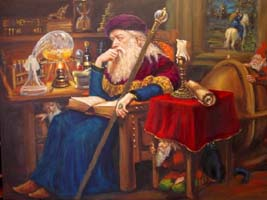
\includegraphics[scale=.5]{a20151111MindandCosmos-img001.jpg}
\end{wrapfigure}

A couple of weeks ago I watched the notorious atheist and Darwinist \textbf{Richard Dawkins} interviewed by a
non-descript host on a cable news network. Since the context was a discussion of Ben Carson's belief in
creationism, the host listened with rapt attention to, but little understanding of, Dawkins' presentation.
Of course, for the half-educated intelligentsia represented by the host, a blind belief in the “theory of evolution” is
a status marker even though they neither understand it in depth nor are aware of its ultimate consequences for human
life and thought.

Without defining the term, Dawkins asserted that “evolution” is a “fact”. We agree that the two basic components of
evolution are facts. These are:

\begin{itemize}
\item \textbf{Descent with variation}: the offspring are similar, but not identical to the parents. 
\item \textbf{Natural selection}: some organisms will reproduce themselves better than others in their natural
environments. 
\end{itemize}
There are subsidiary facts, such as:

\begin{itemize}
\item DNA sequences of similar organisms have many commonalities 
\item The age of the earth seems to be quite old 
\item The fossil record shows organisms arising and being replaced by other organisms 
\end{itemize}

\paragraph{Nagel's Thesis}
There is no point in disputing settled scientific facts. Instead, Nagel himself points out some additional facts:

\begin{itemize}
\item \textsc{Consciousness}: its subjective character has no physical explanation 
\item \textsc{Cognition}: thought and reasoning are correct or incorrect independent of the thinker's
beliefs 
\item \textsc{Values}: values are real, not merely subjective 
\end{itemize}

Properly understood, Nagel shows that these facts cannot be explained by nature understood as simply physical and
material. Nagel is an atheist, just like Dawkins, so there is no question of special pleading for a partisan religious
view. The two components produce different results.

\begin{enumerate}
\item Descent with random variation should work like a random walk\footnote{\url{https://en.wikipedia.org/wiki/Random_walk}}. Specifically, “evolution” is not evolving in a
particular direction, rather, it is probably going nowhere. 
\item Yet that is not what is observed. Instead, nature or the environment seems to channel evolution in specific
directions. 
\end{enumerate}

\paragraph{Antireductionism}
As part of organic life on Earth, man is subject to a multitude of laws. First of all, as a corporeal being, he is
subject to the laws of physics: gravity, conservation of energy and momentum, and so on. Then, he is subject to the
laws of chemistry, since a large number of chemical reactions constantly occur in the body.

However, physical and chemical laws are surely insufficient to understand any form of life, never mind human life. For
example, it would not be possible to understand the movement of people in a city just based on force and momentum. It
is not even possible in principle.

So, why would the “theory of evolution”, as a biological law, be able to explain the totality of the human being? That
is what is objectionable in neo-Darwinism. The facts as such are not in dispute. What is far from obvious is that
genetic variation and natural selection together explain everything about human life. How can DNA cause conscious and
sentient beings?

\paragraph{Chance and Intelligibility}
Nagel begins his discussion with the notion of the intelligibility of the world. That is equivalent to the Principle of
Sufficient Reason, the notion that everything about the world can be understood at some level. Absolute Idealism\footnote{\url{https://www.gornahoor.net/?p=8366}} (e.g.,
Plato, Schelling, etc.) considers rational intelligibility to be at the root of the natural order. So Nagel considers
himself an absolute idealist (but never writes of the Absolute in this book).

Since mind is part of that order, it, too, must be intelligible. Nagel denies that physical, chemical, and biological
laws —i.e., efficient causes alone— suffice to explain mind. Therefore, he is compelled to bring
in the idea of teleology, or final causes, to explain the emergence of mind. That acts as a “pull” to the “push” of
efficient causes. Although he does not express it this way, efficient causes are quantitative while final causes are
qualitative. Since the whole scientific enterprise began with Francis Bacon's rejection of final causes and
Galileo's rejection of qualitative explanations, Nagel in effect rolls back thought to a pre-modern era.

Nevertheless, it is not a simple reaction against the modern world, since it also incorporates whatever truths modern
science has given us.

Unfortunately, while science has promised to make the world intelligible, it has done so by leaving out important
features. First of all, the opposite of intelligibility is chance or randomness. In fact, a random sequence is such
because the next element of the sequence cannot be inferred from any of the preceding elements. Perfect randomness\footnote{\url{https://www.gornahoor.net/?p=4970}},
therefore, is the denial of the Principle of Sufficient Reason.

\paragraph{Cosmos}
Every outdoorsman knows that a random walk in the woods leads nowhere; most likely, you would end up close to where you
started. That is why you need to mark your path so you don't traverse the same places twice. Hence, if a
city boy was lost in the woods, but emerged two days later, you might call that a miracle. Or else, you might suspect
he had some skills he hadn't owned up to.

That is the situation as Nagel sees it. The emergence of conscious, intelligent, and rational beings by chance alone
does not seem at all plausible. Now, the first factor in evolution, viz., variation or genetic drift, is certainly
random. If it follows a random walk, it should go nowhere. Fossil records should show species evolving backwards to
more primitive forms, for example. In other words, there is no “direction” to evolution, or, in other words, no
teleology.

On the other hand, the second factor, natural selection, is not random. Dawkins himself did an experiment with
Scrabble-like tiles. By randomly placing the tiles, followed by a selection mechanism, he would end up with an English
sentence\footnote{\url{https://www.gornahoor.net/?p=8253}}. In his example, Dawkins was the intelligent selection factor.

So if life as we know it is the result of random variations and natural selection, Nagel explores the selection factor.
Specifically, what would nature have to be like to produce human beings?

\paragraph{Consciousness}
Nagel endeavors to explain three facts: the emergence of \textbf{consciousness}, \textbf{cognition}, and \textbf{value}
in biological species. As a committed naturalist, he rejects theological explanations that account for those facts from
a force outside nature. That is fine since the general understanding of God in exoteric religious adherents is usually
defective, creating as much confusion as insight. Likewise, he rejects reductive naturalism that, in effect, denies the
three facts rather than explains them.

The distinctive feature of consciousness is its subjective, or we would say qualitative aspect. There is no explanation
of conscious experience in terms of physical laws. While brain states may empirically be shown to create certain
experiences, that opposite is also true. Consciousness can likewise affect brain states.

This all seems difficult for some to accept. A diehard reductionist will rely on behavioristic explanations. For
example, if an organism responds to a flash of light, that behavior is an indication of consciousness. In that view,
then, there is nothing to explain. Similarly, human beings will “report” having certain sensations and experiences. The
reporting is all that matters.

Yet that misses the essential point, viz., the subjective aspect of consciousness, which it attempts to make objective.
Are the automatic doors at the supermarket conscious in any sense? According to the behaviorist criterion, perhaps they
are. So why do we believe an octopus is conscious but not a door?

Nagel concludes, then, that \emph{mind is an essential part of nature}, not a byproduct of material processes. This is a
form of panpsychism.

\paragraph{Cognition}
Nagel then turns to “cognition” as he calls it, which appears in the human being. Metaphysically, the human being is
characterized by “intelligence”, which is different from seemingly intelligent activity in animals. Specifically, Nagel
defines cognition as “the functions that have enabled us to transcend the perspective of the immediate lifeworld given
to us by our sense and instincts, and to explore the larger objective reality of nature and value.”

Thought and reasoning are correct or incorrect in virtue of something independent of the thinker's beliefs.
Logic, mathematics, and metaphysics are timeless, hence immaterial. This is reminiscent of a more sophisticated version
of C. S. Lewis' Argument from Reason\footnote{\url{https://en.wikipedia.org/wiki/Argument_from_reason}}. Cognition certainly cannot be explained solely in terms of behavior.
And it should sound odd that a life form would arise that would seek to understand its own origins.

Now a reductionist may try to refute this in a couple of different ways. One is the emergence of serendipitous uses for
features that evolved because of reproductive fitness. For example, a hand came to be used by a Michelangelo to create
beautiful art. Certainly, that in itself has no reproductive value. But that inadvertently confirms an earlier point:
biology alone cannot explain everything about the human being.

Another is the obvious and glaring lack of logic and rationality in the human race. Evolutionary psychologists have
noted many of the logical fallacies and irrational beliefs of humans. Nevertheless, they have biological fitness. True
rationality, then, is just a special case of the origin of thinking.

It is rather odd that false ways of thinking lead to reproductive success. The rare thinking occasions involving
objective truths probably have little reproductive success. For example, try discussing this review on your next date;
I can guarantee you will spend the night alone. Moreover, the most scientifically advances societies usually have
negative birth rates\footnote{\url{https://en.wikipedia.org/wiki/Population_decline}}.

\paragraph{Values}
Nagel then points out the existence of objective standards of value: good and bad, right and wrong. This he calls “value
realism”. Again, he claims that objective values make no sense in a materialistic universe. Things are good or bad not
because genetically determined behaviors lead to the preference of one thing over another.

Human action involves more than physiology and desires, it requires judgment. Clearly, then, this requires “free will”,
or the ability to make a moral judgment.

Nagel shows the richness of absolute idealism in retrieving a deeper, more human, view of the cosmos, beyond the
materialist reductionism that dominates educated thinking today. Nagel accomplishes this while fully incorporating
scientific knowledge.

Mind, consciousness, intelligibility, rationality, judgment, free will, are all restored in a more comprehensive
understanding of the cosmos. Nagel does this sparingly, a type of philosophic minimalism, with no brick that is not
essential to the edifice he has created.

\flright{\itshape Posted on 2015-11-11 by Cologero}

\begin{center}* * *\end{center}

\begin{footnotesize}\begin{sffamily}

\texttt{Mercurius on 2015-11-13 at 23:08 said: }

A clear, intriguing, and captivating review Cologero, stimulating much interest in reading the five or so major titles
you've been lately discussing, between here, in “The God of Metaphysicians”, and “Spiritual Regeneration”
posts.

Though Nagel is, as noted above, an “atheist” (maybe better really, a non-theist), there is something serious to be
noted in a “modern” science which begins to consider, and recognize, that consciousness is a sort of fundamental
universal constant. Independent and objective, even in the most “materialist” constructs–which then really, changes
everything.

Brings to mind, a small passage in Kingsley, where he exclaims:

“The Iatromantis was someone who was a master of the state of awareness. Waking is a form of consciousness, dreaming is
another. And yet this is what we can live for a thousand years but never discover, what we can theorize or speculate
about and never come close to–consciousness itself.

Its what holds everything together and doesn't change”.

That is Kingsley, but in two beautiful passages, Emperor Aurelius, and Shopenhauer seize upon the same state–creating
“reboot” points, within the Western cannon.

Related, is an interesting, and recent drive, within physics, to in fact address the “c” issue, keeping it within well
enclosed constraints of “materialism”–considering it as indeed, a “panpsychic” element of nature–but entirely, at the
same time, while avoiding ideological conflicts, seeking to stuff in into gross biology–curious nonetheless, to even
BEGIN regarding consciousness as a “state” of “matter”, on par with accepted “states”. 

Perhaps not quite “traditional”–but, maybe with some modifications, at least for an exoteric sake, these ides of
consciousness can find assimilation with Samkhya, Greek “atomism”, and Stoic “Logoism”?:

\url{https://medium.com/the-physics-arxiv-blog/why-physicists-are-saying-consciousness-is-a-state-of-matter-like-a-solid-a-liquid-or-a-gas-5e7ed624986d}


\hfill

\texttt{Olavsson on 2015-11-14 at 12:55 said: }

While this work of Mr. Nagel seems highly valuable, something worth reading in order to improve one's
understanding of what a contemporary, “up-to-date” so to speak, refutation of various fundamental modernist assumptions
about humanity, consciousness, evolution and the world might look like, there is something here which makes his
`perspective' deviate from fully qualifying as Absolute Idealism, don't you think?
In his worldview, the notion of “nature” still seems to be of supreme centrality, although he accepts consciousness as
an inherent, not merely accidental and contingent, “part of the picture.” Is there a presence of actual transcendence
within this worldview, which would make “nature” itself merely one of several aspects of particular “states” of the
total Being rather than the supreme reality per se? While Nagel's understanding certainly is a vast
improvement to the reigning scientific paradigms, as far as integrating Idealism is concerned, it still seems to
preserve a concept of an independent “nature” that didn't really exist anywhere in the Traditional world.
But I might have misinterpreted. Certainly worth a read in any case.

I have not been able to follow Gornahoor as much as I'd like to during the last months as my access to
internet is limited and there's been other things demanding my attention, but I will now try to comment
more, and hopefully participate in one of your Gnosis cycles.

I must repeat what I've said before, that this website offers something truly unique to those on a quest for
truth in the west today.


\hfill

\texttt{Cologero on 2015-11-18 at 18:37 said: }

Olavsson, Nagel referred to the absolute in a passing comment and, apparently, it was not necessary for his argument. He
restricted himself to a form of naturalism. That is probably the most effective approach in our time, since overtly
religious or complex metaphysical schemes are beyond the pale for the educated classes.

Since he mentioned Schelling, that is where we should probably look for a fuller picture. By extrapolating
Nagel's thesis, the physical world does not form the ground of consciousness. Conversely, consciousness
does not “create” the material world. This avoids dualistic solutions. If the mind is part of the world, then
man's mode of being in the world is as a conscious body. So, neither matter nor mind is fundamental; hence,
for Schelling and presumably Nagel, the Absolute is their common ground.

This is also more Tao like: the Abolute as Tao, and mind/matter as male/female or yin/yang.


\hfill

\texttt{Olavsson on 2015-11-22 at 12:57 said: }

Cologero: Yes, I think his approach somewhat focused on the level of naturalism may be useful for countering the gross
materialism dominating the secular pseudo-elite of modern civilization. It is imperative that views more closely
resembling idealist philosophy, in contact with science and `updated' to the current situation,
are made relevant again. On a personal level, however, I am mostly concerned with inner realization and what
traditional doctrines mean for my own path to higher spirituality, so the question of which approach is most effective
and influential on the collective level of academia, the scientific community, culture etc, is of secondary importance;
and it is in that other capacity I find Gornahoor's contribution most appreciable.

Regarding the question of the relationship between consciousness and the so-called material world: Wouldn't
it be correct, from the point of view of traditional metaphysics, to assert that Mind, in a supra-individual sense, is
indeed prior to “the world”? Of course, it is not the conditioned consciousness of individual beings existing in the
world that has `created' that world. Isn't it rather the case of individual mind,
such as that of the fallen humans we know, having its ultimate origin in the ideal primordial Mind (in some traditions
the `Buddha Mind’), from whose emanation the relative existences typical of the limited minds
arise, which are in turn conditioned by and co-dependent on the `world' which is a part of
their state of being, a `world' that is not self-existent? That the mind
`creates' the `world’, of course, can only truly be said if we speak of
a `higher' Mind that is not conditioned to be co-dependent on that world, or rather state of
being. It doesn't count for the grosser levels of individual mortal consciousness still subject to cyclical
existence. To say this is not dualism; it is the same principle as when you have stated that “the subtle rules the
dense.” If we accept the traditional possibility of spiritual liberation from the conditions of this
`world', as a state of being, then the conclusion that Mind, if integrated with the ultimate
truth of its origin, is superior to material existence, not just two sides of the same coin, is inescapable. Just to
avoid misunderstanding: I'm not trying to correct you, only throwing some spontaneous reflections out
there. I don't think we disagree here in terms of ultimate principles when looking beyond different
wordings in one specific context. Since the individual minds that we know all experience the same
`world', they do not all `create' it in the sense of some arbitrary
illusive projection from their own subjective starting-point; it obviously has a cause beyond their subjective
experience, now corresponding to a very conditioned form, extremely reduced even compared to the Primordial State
(which is still too conditioned to corresponds to the state of one fully awakened and liberated). So in order to find
the `Mind' that is indeed superior to and more Real than material existence, such lower,
conditioned minds would have to be transcended. The material world does not form the ground of this ordinary
consciousness as commonly believed today, as you point out, because its true `ground' from
which it is emanated or `reflected' is transcendent, but nevertheless, because of this
`reflection' in the lower `waters', these minds now find themselves
conditioned by this `world’ – which is why the materialists believe that the very principle of
consciousness originated from these conditions, in which case no higher freedom would be possible. Likewise, the
material `world' itself is conditioned by consciousness, albeit in a higher sense, as it would
not exist outside of conscious experience, since we are, in this metaphysical perspective, dealing with a state of
being, not just objective “stuff” existing by itself “out there.” I believe this is the best view (though here
expressed simply and not with the subtlest profundity) on the co-depending relationship between consciousness and
matter. On the one hand, you have the facts of our experienced consciousness “here and now”, which is manifested in
certain conditions and may be affected by them, and on the other hand, the higher possibility of consciousness in an
ideal sense. If a state very close to the Absolute may actually be attained through the realization of a being, which
is affirmed by the highest initiatic doctrines (for example Buddhahood, diamantine and indestructible, even in this
life having realized its centre beyond life and death), then mind must somehow be more fundamental than matter, since
matter, as in a stone, cannot serve as the starting-point for a transcendence of its own condition, while mind can. The
point is: the mortal mind needs these material conditions to operate as long as this state of being lasts, of which
matter is one of the relative, dependent conditions, but consciousness may use these conditions as a springboard to
reach beyond them, and the mind-stream will outlast the death of the physical constituents, though in a different form.
This, of course, does not hold as an argument in debates with materialists, since certain metaphysical premises must
already be accepted as true. That is usually the approach I choose to take, since I'm not so much
interested in finding common ground on which to debate with materialists as I am in realizing for myself what walking
the path of the sages of old has to offer a being today.


\hfill

\texttt{Cologero on 2016-08-30 at 19:38 said: }

Update on science.\newline
Note the claim that we made in this post:

\begin{quotex}
Instead, nature or the environment, \emph{seems to channel evolution in specific directions}. 

\end{quotex}
Compare that claim to this most recent scientific findings, of which I was just made aware:

\begin{quotex}
Rather than genes simply “offering up” a random smorgasbord of traits in each new generation, which then either prove
suited or unsuited to the environment, it seems that \emph{the environment plays a role in creating those traits in
future generations}. 

\end{quotex}
The full article is available at \textit{Why everything you've been told about evolution is wrong}\footnote{\url{https://www.theguardian.com/science/2010/mar/19/evolution-darwin-natural-selection-genes-wrong}}.

This shows that metaphysical principles can provide information even before it can be verified empirically.

\end{sffamily}\end{footnotesize}

\section{Esoteric Darwinism}

I spent a few hours this week reading some reviews of \emph{Mind and Cosmos} by \textbf{Thomas Nagel}; I
hadn't realized it was such a widely reviewed work. There are some broad categories of reviews. After
briefly describing them, I will offer the esoteric interpretation. Finally, we will explain why Zarathustra was so
frustrated.

\paragraph{Materialism}
\begin{wrapfigure}{rt}{.35\textwidth}
 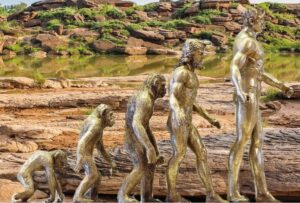
\includegraphics[scale=.5]{a20151116EsotericDarwinism-img001.jpg} 
\end{wrapfigure}

There are the diehard materialists who reject the argument \emph{a priori}. The objection is to the introduction of
“mysterious” forces like mind, teleology, and so on. I suppose that familiarity breeds contempt, since gravity,
electromagnetism, quantum mechanics, the big bang, the origin of life, etc., are themselves quite mysterious. Moreover,
the claim that “matter” follows “laws” is itself an indication that there is intelligence inherent in matter. On the
other hand, consistent positivists like Stephen Hawking admit that scientific theories have merely pragmatic value, but
tell us nothing about ultimate reality.

Ultimately, there is no way to resolve the conflict between materialism and idealism in thought alone. What the latter
finds intelligible, the former considers just a serendipitous sequence embedded in a purely random sequence. It seems,
also, that it is impossible for real materialists to consider subjective conscious experiences of any significance. It
really comes down to differences in people and how they experience inner states. Some just don't seem to
have a very vivid interior life.

\paragraph{Sympathetic Views}
There are broadly sympathetic views. However, they don't seem to share Nagel's viewpoint;
rather, they latch onto the criticisms of neo-Darwinism. Nagel himself describes his point of view this way:

\begin{quotex}
The view that rational intelligibility is at the root of the natural order makes me, in a broad sense, an
idealist —not a subjective idealist, since it doesn't amount to the claim that all reality is
ultimately appearance— but an objective idealist in the tradition of Plato and perhaps also of certain
post-Kantians, such as Schelling and Hegel, who are usually called absolute idealists. 

\end{quotex}
I couldn't find a review by an “absolute idealist”; perhaps there aren't any left. Nagel claims
that absolute idealism was simply abandoned, not refuted.

Curiously, a Thomist thinker wrote that Nagel's view is an “essentially neo-Aristotelian position”. It would
be interesting, but also welcome, to classify neo-Aristotelians among the absolute idealists. The idealists
I've read would certainly have benefited by the inclusion of Aristotelean elements, in particular,
hylomorphism. Certainly, Julius Evola did so with great effect with his ideas about essence, existence, and privation.
For Rene Guenon, too, the notion of the Absolute was fundamental. Certainly, he combined ideas from the Samkhya school
(purusha/prakriti) within his Vedantic approach.

Absolute idealism starts from “above”; i.e., it begins with the notion of the Absolute and derives the world.
Aristotelianism starts from “below”, with sense experience, and by analogy reaches the Absolute.

\paragraph{Neotheism}
There is a view called Neotheism, which considers God as a very powerful being among other beings, rather than as the
Absolute or Being itself. Actually, this is the idea of God in the popular mind, rather than the true classical idea.
Even atheists, for the most part, refute such a neo-god, thereby missing the point. If such a being exists, then there
is still the Absolute – rather confusing.

Although this group likes Nagel's critique of neo-Darwinism, it is really not very helpful. In effect, this
view is not unlike the naïve realism of the materialists: the world is out there, right now, in some spatial container
in time. However, they then presume that the neo-god provides the goal and meaning to this space-time material world.
The world in itself is meaningless, just as it is for the materialists. They add to this world invisible beings and
miracles that seem to come from nowhere.

\paragraph{Mystical Evolution}
It seems, then, that we are faced with an impossible dilemma: accept science or accept a spiritual life. On the other
hand, \textbf{Valentin Tomberg} gave us the teaching of Practical Monism, which reconciles, or neutralizes, the pair of
opposites. However, that is accomplished not in the realm of speculative thought but rather in practical reason. That
is, it is only by living, not just by thinking, that the dualism in thought is resolved in a practical monism.

The materialist view is consistent with esoteric teaching. For example, \textbf{Boris Mouravieff} writes this in
\emph{Gnosis}, Vol 1:

\begin{quotex}
Properly speaking, this kind of existence cannot be considered as human; it could be described as anthropoid. This term
is justified in the sense that exterior man, immersed in self-satisfaction, represents the crowning achievement of
millions of years of evolution of the species from its animal ancestors, yet, from the point of view of esoteric
evolution, he is a possibility which has not yet been realized. 

\end{quotex}
So the scientific teaching that man, as he is, is an ape, an anthropoid, is consistent with esoteric teaching. Like all
animal life, the anthropoid man is under the dominance of the General Law of fear, sex, and hunger. All his ideals are
illusory epiphenomena, supervening on a bed of genetic, libidinal (Freud), and economic (Marx) forces.

That is the first birth. The initiation into the true life of the spirit is the second birth; the anthropoid gives birth
to the man as he should be. He seeks to overcome the general law of biological life in order to realize his True Self.
This is not an automatic or material process. Rather, it must be freely chosen and it requires conscious efforts. In
other words, he becomes his aim in life.

\paragraph{Zarathustra}
\begin{quotex}
Transformed is Zarathustra; Zarathustra has become a child; an awakened one is Zarathustra: what will you do in the land
of the sleepers?

I love him who lives in order to know, and seeks to know in order that the overman may someday live. \flright{\textsc{Friedrich Nietzsche}, \emph{Thus Spoke Zarathustra}}

\end{quotex}
Just as in the case of Galileo, people have heard rumors about Darwin, but its meaning has not yet sunk in. For the
educated it is important to “believe in evolution”. But to believe that, is also to believe you are an anthropoid. Yet
the modern man believes that he is the goal of evolution, its acme, and that nothing could be conceivably be higher.
Thus he is the last man and proud of it. If everyone would be just like him, the Kingdom would arrive and the evil ones
would be transported away on a cloud. There would be no war, no global warming, and so on.

So Zarathustra told them they were anthropoids, since they should want to know. Instead, they banished him, because in
the Country of the Blind, the seer is a menace.

\flright{\itshape Posted on 2015-11-16 by Cologero}


\chapter{The Foundation of the Modern World}
\section{The Truth is far from Suspected}

\begin{quotex}
Be assured, savants of the world, it is not in disdaining the sacred books of nations that you show your knowledge, it is in explaining them. One cannot write a history without monuments and that of the world is no exception. These books are the veritable archives wherein its deeds are contained. It is necessary in exploring the venerable pages to make comparison between them and to understand how to find the truth, which often languishes there covered by the rust of ages. \flright{\textsc{Fabre d'Olivet}}

\end{quotex}
In our task to identify the sources of the ``formidable mental deviation that characterizes the modern west" [\textbf{Rene Guenon}], I took one for the team and endured a ``debate" on youtube between the two Christophers — Hitchens and Hedges. It was advertised as the contest between two worldviews: the scientific one represented by Mr. Hitchens and the religious by Mr. Hedges, although, in point of fact, they more or less agreed on everything. What is more remarkable, however, is their unexpected, and probably unwelcome, agreement in many respects with séance meeting spiritualists as described in Renen Guenon's \textit{The Spiritist Fallacy}.

There is no value in getting involved in such debates if only for the most basic reason that it assumes a common intellectual plane for such a debate to occur. Nothing could be further from the truth since what would be necessary is the questioning of fundamental assumptions. The religious point of view in that debate involved too many disparate and incompatible notions; to do it properly would require the translation of the religious dogmas to their metaphysical equivalents. Only then could there be a fruitful discussion apart from the obvious difficulty that few would be capable of engaging in such a discussion for a variety of reasons.

The modern worldview represented by the Chrises must start from the assumption that the past is no more than a period of darkness, ignorance and depravity that can only be redeemed by modern ideas. Regarding the study of the past, Guenon writes:

\begin{quotex}
History, as officially taught, limits itself to exterior events, which are only the effects of something deeper; and it sets these events forth in a tendentious manner under the influence of all the modern prejudices. And further, there is a veritable monopoly on historical studies in the interest of parties, both political and religious. 

\end{quotex}
The Hermetic method of doing history as described by Fabre d'Olivet, whose influence on Guenon is undeniable, is quite different. To grasp the world of the ancients expressed through their sacred scriptures requires a deep understanding of their essences which is revealed in their homogeneity rather than simply in the outward events described. To disdain those writings and neglect their truths is to limit oneself to the parochialism of the present. Even more than Guenon, who mined such texts for their symbolic and metaphysical value, \textbf{Julius Evola} made use of myths, legends, and sacred texts to discern the worldview of the ancients. Regarding the deprecation of that worldview or the deliberate ignorance of it, Guenon writes:

\begin{quotex}
This falsification of history seems to have been accomplished according to a set plan; but if this is so, and its essential aim has been to have public opinion consider this deviation as `progress'. everything seems to indicate that it must be the work of a directing will. … in any case, it can only be a collective will, for there is manifestly something that goes beyond the sphere of activity of individuals considered in isolation. 

\end{quotex}
First of all, let's be clear about the more or less common opinions held by the modern mind. It is characterized by appeals to humanitarianism, moralism, or sentimentalism, rather than anything properly intellectual. They envision a world of pacifism, universal brotherhood, various ``rights", liberation, and so on, all to be brought about in a more or less distant future. All of this is couched in the guise of ``progress" and ``evolution" and allegedly backed up by science. Guenon describes its effects:

\begin{quotex}
One can hardly imagine the seduction that grand words offering a false semblance of intellectuality exercise … This is a kind of verbalism which provides the illusion of thought for those incapable of really thinking; it is also an obscurity which passes for profundity in the eyes of the common man. 

\end{quotex}
There is little chance for intellectualism to gain any headway in this discussion. To those accustomed to live only by their passions and their arbitrary ``likes", a commitment to the intellect seems oppressive to them, rather than the true liberation that it is. The appeal to Tradition is associated with the defects of the known past. On an emotional level, that can only fall short of the imagined glories of the unknown future.

What is really curious about all that is how that modern worldview arises as the conclusion of disparate premises. For example, spiritualists and the ``new atheists" come to the same conclusion, although the latter abjure the former. New Agers, liberal Christians like Hedges, socialists, and so on all agree on that worldview. In other words, it matters little the exterior religious or philosophical allegiance, so long as the result is the same. This leads Guenon to this suspicion:

\begin{quotex}
If one does not believe in chance, one is forced to admit the existence of some kind of equivalent of an established plan, but one which evidently does not need to be formulated in any document. Isn't the fear of certain discoveries of this kind one reason for the superstition of the `written document' as the exclusive basis of the historical method? Starting from there, all that is essential necessarily escapes investigation. 

\end{quotex}
Once again, we see that understanding history requires determining the essence behind the appearances. Since that cannot be determined from written documents, it is rejected by ``official" historiography which is based on texts. Hence, any mention of a ``plan" is ridiculed as a conspiracy theory. This is exacerbated by the fact that most people are merely the unconscious instruments for the plan's effectuation, so they can plausibly deny it. Of course, Guenon is not some simple-minded conspiracy theorist. He elaborates:

\begin{quotex}
It is impossible to believe in the spontaneous production of movements of any importance. In reality, things are more complex than we indicated; instead of a single will, we should envisage several intentions as well as several results; there could be a whole special dynamic in this, whose laws would be interesting to ascertain … the truth is far from being generally known or even suspected. 

\end{quotex}


\flrightit{Posted on 2013-01-02 by Cologero }

\begin{center}* * *\end{center}

\begin{footnotesize}\begin{sffamily}



\texttt{Jason-Adam on 2013-01-02 at 23:40 said: }

I'm currently reading Fabre d'Olivet's book right and clearly see the huge influence it had on Guenon \& Evola – though obviously more on Guenon…………

In studying the history of ideas one needs to understand that the person said idea usually had an end in mind beyond inocuous speculation….by discovering the hidden ends and means we unravel history.


\end{sffamily}\end{footnotesize}

\section{The Future They Hope for}

\begin{quotex}
What inspired Teilhard de Chardin, and inspires his followers, is a certain unitary view of reality, a joining of God and the world, of the spiritual and the secular, into a single harmonious and all-encompassing process which can not only be grasped by the modern intellectual, but can be felt by the sensitive soul that is in close contact with the spirit of modern life; indeed, the next step of the process can be anticipated by the modern man, and that is why Teilhard de Chardin is so readily accepted as a prophet even by people who do not believe in God: he announces, in a very mystical way, the future which every thinking man today hopes for. \flright{\textsc{Fr. \textbf{Seraphim Rose}}}

\end{quotex}
Since we never got to the actual debate between the Chrises yesterday, we can try to mention the main points. Neither of the men are very deep or careful thinkers. As Fr. Rose points out, they share a common vision of the future, something they ``feel" more than ``think", despite their radically different starting points. They are the heirs of currents of thought that began centuries ago, which they now accept uncritically.

The best thinkers, those who laid the foundation for the modern world, dig down to the roots of thinking. By rejecting Euclid's famous fifth postulate, geometers were able to create alternative geometries. In an analogous way, certain thinkers rejected one or another of the fundamental concepts of Traditional metaphysics, and drew out all the consequences thereof. We have provided the examples of Francis Bacon who rejected formal causes, Spinoza rejected final causes, and Nietzsche proclaimed the death of God. They are not necessarily the conscious agents of change; more likely, they simply can't understand, or intuit, the point of traditional teachings.

Over time, the professors pick up these ideas, their students accept them uncritically, until eventually certain ideas enter the public realm; the conclusions are adopted although no one any longer understands how they came about. The common element is the revolutionary idea and opposition to the status quo. Several years ago, a secular friend married a spiritualist. She told me she was an ``iconoclast". I recall that I thought it was quite a strange thing to say. I pointed out that her husband was a real iconoclast, but he didn't have to boast about it. That ended that friendship.

I wonder how she feels now that the revolution is firmly in control, so it makes no sense to smash the idols. Of course, like the ancient Hebrews and Greeks, mere victory is insufficient; every man, women, child, livestock, and edifice must be destroyed. That is why the modern mind is so rabid and intolerant of any opposition to their imaginary future.

When someone argues very emotionally and illogically, you can be assured their point of view has little validity. That is Christopher Hitchens. Unlike Nietzsche's atheism, with its attendant transvaluation of all values, Hitchens' new atheism is rather tame, and actually unnecessary to his point of view. As we pointed out, his anti-clericalism and progressivist view is common to spiritualists, new agers, and others who may not share his atheism.

He does not think deeply, but instead begins in the middle with unexamined assumptions. A frequent theme is that religions are man-made creations. From a certain perspective, that is true especially if history is considered as no more than the examination of written texts as Guenon points out. What Hitchens doesn't mention is that scientific theories are likewise man-made creations, subject to change and refutation. Unlike religious texts, a scientific text can claim no higher authority, so it serves as a shaky basis for a worldview. Of course, that worldview claims that knowledge is progressive; so if it is admitted that what science teaches now is incomplete or even false, why should we accept anything now?

Hitchens' main point is that he adheres to a higher morality. He thinks that because he is under the illusion of ordinary life and simply cannot conceive a contrary point of view. The deeper question is why be moral at all? Morality makes no sense in his atheistic worldview. One can only be moral out of habit, inculcation, or from blindly accepting the imperatives of one's genetic programming. He fails to grasp that his moral and political views have no necessary connection to his atheism and belief in science.

He rants quite a bit, all in support of a progressivist worldview and in opposition to all religions which he lumps together. Of course, he does not allow the opposite, refusing to be linked to the nefarious actions of other atheists. He was obsessed with the treatment of menstruating women in Jewish law, but his point is unclear. While we don't think it right to banish such women from the public square, it is certainly not something to embrace. But that brings up a point. If you accept the premises of evolutionary biology, then feelings of revulsion must have a survival value. Nevertheless, he seems to praise practices that evoke such feelings in normal men.

There is a final point. Science is based on careful study of the past, from which hypotheses are derived. For example, Tycho Brahe spent decades tracking the motions of the planets; that allowed Kepler to formulate his laws of planetary motion. Similarly, the understanding of human nature, as a science, must begin with the study of history, from which an anthropologist can propose general laws. Since the future is everything to Hitchens, he departs from true science by ignoring the past. He proposes, in his utopian vision, revolutionary changes in social arrangements, changes which may never have been tried in the past. A real scientist, it seems to me, would be much more cautious about advocating such changes without first understanding all the ramifications.

Hedges was a non-entity as the foil. The only remnants of his Calvinist background that he retains is a dour personality and a belief in total depravity. Apart from that, the two Chrises agree on the revolutionary future. Hedges sincerely believes that the religious right is the greatest danger in the USA. In actuality, the religious right has been politically ineffective as they lack the intellectual chops to oppose the revolution effectively. For Hedges, they are nevertheless the tattered remnants of throne and altar, or the windmills of imaginary fascism that he thinks he is jousting.



\flrightit{Posted on 2013-01-03 by Cologero }

\begin{center}* * *\end{center}

\begin{footnotesize}\begin{sffamily}



\texttt{Mihai on 2013-01-04 at 10:09 said: }

It seems to me very relevant that the only people from the religious ``side" who are called to such debates are protestants and neo-protestants or at least progressive types in general- such as Vatican II Catholics. 

Since you mentioned Fr. Seraphim, he is very accurate in pointing out that Christians with an evolutionist/progressist worldview are extremely immature in thinking that simply adding God to the whole evolutionist paradigm ``solves" the problem. I've read even the statements of an orthodox monk who thinks there is no problem with darwinian evolutionism as long as one puts God as the cause of the process. 

Certainly, Christians who think like this, especially the ones who spend extended time with Scripture, like the monk above, suffer from a certain ``hardening" of the intellect when making such statements. And I am not saying this as an insult or an exaggeration. Clearly they did not spend a single moment to trully ponder the implications of such a worldview. For example: can anyone explain to me, in the light of evolutionism, the first 11 chapters of Genesis ? Or what is the purpose of the birth of Christ, who came to halt history's decline, if we are to accept no such decline, but on the contrary, an unconscious and impersonal evolution ?

And what about the description of the end times, which are represented as a period of utmost degeneration ?


\hfill

\texttt{Matt on 2013-01-04 at 12:03 said: }

Mihai,

That monk may have been speaking about evolution (genetic change) without the neo-darwinian framework attached to it that disregards formal and final causes. However, if he is speaking about it with the framework in mind, then yes, the problems are merely pushed to the side.


\hfill

\texttt{Michael on 2013-01-04 at 14:56 said: }

Mihai,

Of course you know the problem is that virtually all scientists teach the evolution of man. Do you believe that the theory of evolution will one day fall into disfavor as we learn more about our past?


\hfill

\texttt{Mihai on 2013-01-04 at 16:27 said: }

@Matt: Genetic change is one thing and evolutionism is another. Of course, these two things are confused with one-another, or people falsely assume that genetic changes ``proove" evolution, which is why we have this problem in the first place.

@Michael: The problem is not about the study of the past. It is about the worldview. Evolutionism was the dominating paradigm of the western world way before Darwin formulated his theory. This is not a scientific fact, it is a philosophical formulation. The large public (and indeed many scientists) cannot tell the difference between these two domains and this is why evolutionism is at the very hub of the modern mentality.


\hfill

\texttt{Cassiodorus on 2013-01-04 at 16:33 said: }

I've been reading some interesting material featuring the on going debate between the Intelligent Design community and Thomist defenders of theistic evolution. I finally understand the difference: the ID people have larglely accepted the premises of the materilaist's mechanical philosophy whereas the Thomists staunchly remain true to immanent teleology and Aristotelian formal and final causes.

I keep wondering if their is something about Scholastic moderate realism that made the surrender to nominalism something of a forgone conclusion.


\hfill

\texttt{Cologero on 2013-01-04 at 23:56 said: }

{\textgreater}{\textgreater}"I keep wondering if there is something about Scholastic moderate realism that made the surrender to nominalism something of a forgone conclusion."

Perhaps in the sense that non-Euclidean geometry is the conclusion to Euclidean geometry. There is no logical connection. Nominalism is the forgetting of the ideas. For the Scholastics (and beyond) to know is to know the essence or idea of the thing. When that no longer makes sense to anyone, nominalism is the result.


\hfill

\texttt{Noct on 2023-01-03 at 10:30 said: }

Evolution cannot be real because the greater is not derived from the lesser, it is the same narrative of the tower of Babel and progressivism in general. Pretending to reconcile religion and modern science is an absurdity that only leads to the corruption of traditional understanding by giving ground to materialism.

The ape is not potentially a man, and to involve God as an explanation of the process is to ignore causality for a simple evolutionary bias. God does not magically add new genes, mutations cannot mean a qualitative progression, every actualization depends on an already existing potentiality. The lesser does not contain the greater, but the greater always contains the lesser. Species do not evolve, but degenerate.


\end{sffamily}\end{footnotesize}

\section{Francis Bacon and the Creation of Modernity}
\label{sec:BaconModernity}
It is our contention that great events in world history are deliberately planned; nothing happens at random, and things happen for a reason. To understand such reasons is the very definition of intelligence. The beginnings of the modern mind were found in the anti-metaphysics of nominalism. But it was \textbf{Francis Bacon} who sketched out the intellectual lineaments of modernity and, in the process, redefined what it means to be an “intelligent” man. His definition still holds today among the university educated and is even absorbed unconsciously among the masses.

Bacon lays out his plan in the Great Instauration, an ironic reference to Ephesians 1:10, “to instaurate everything in Christ”. We must not be deceived by Bacon's pious language and Biblical references which are included to mask his true intentions, as the consequences of his method had to have been known to him. To deny that is to deny Bacon's intelligence; Bacon was anything but unintelligent. The consequences of his plan will be the denial the supernatural from any understanding of the world. Bacon reveals his purpose in the Preface:

\begin{quotex}
That the state of knowledge is not prosperous nor greatly advancing, and that a way must be opened for the human understanding entirely different from any hitherto known, and other helps provided, in order that the mind may exercise over the nature of things the authority which properly belongs to it. 

\end{quotex}
\begin{enumerate}
\item \textbf{Problem}: The state of knowledge is not advancing. 
\item \textbf{Solution}: A way of knowing entirely different from anything in the past. 
\item \textbf{Benefit}: The mind exercises its authority over the nature of things. 
\end{enumerate}
The attack on Tradition is made head-on. The Traditional view is totally opposed.

\begin{enumerate}
\item The can be no advancement of Traditional knowledge. 
\item There is nothing new under the sun. 
\item The nature, or essence, of things has its authority in the mind of God. 
\end{enumerate}
Bacon masks his intentions by claiming to be returning to the Primordial State, when Adam was given dominion over the world. But Adam's naming of the animals was an act of recognition, a remembering of their nature or form. Bacon, despite his protests, takes on the Satanic project of replacing God, so that the new man is now the arbiter of forms. This is not a moral judgment, but rather a description. To know what a thing is, is to know its sufficient reason. The Western Tradition lists four causes to explain a thing or event, as shown in Table~\ref{tab:fourcauses}.

\begin{table}[h]
\small
\label{tab:fourcauses}
\centering
\begin{tabular}{lll}\toprule
\textbf{Cause} &
\textbf{Description} &
\textbf{Question}\\\toprule
Material &
What something is made of &
\\\midrule
Formal &
What it is &
What\\\midrule
Efficient &
How it came to be &
How\\\midrule
Final &
What is its purpose &
Why\\\bottomrule
\end{tabular}
\caption{The traditional doctrine of four causes}
\end{table}

Bacon takes his stand against this schema by first rejecting the final causes. He explains why:

\begin{quotex}
I am laboring to lay the foundation, not of any sect or doctrine, but of human utility and power. 

\end{quotex}
Hence we see that everything must be in service to human utility and power. If anything has its own reason for being, that is, its formal cause, then its usefulness for human ends is no longer the prime consideration. He then rejects the notion of formal cause:

\begin{quotex}
Matter rather than forms should be the object of our attention, its configuration and changes of configuration, and simple action, and laws of action or motion, for forms are figments of the human mind, unless you call those laws of action forms. 

\end{quotex}
Can it be said more clearly? Only matter, its configurations, changes, and actions are to taken into account. There is no hylomorphism and hence the natural world is not the reflection of the supernatural. There is a subtle change in the notion of the efficient cause. It no longer refers to the essential and internal relationship between forms, but rather to the accidental and external relationship between material configurations. Now Bacon calls the alleged intuition of forms a ``figment of the imagination''. This is why we insist that debate is pointless. If a man can see the forms, or ideas, it is no figment; otherwise, it may as well be. Philosophical discussion can make the concept plausible, but only gnosis can prove it. Let us make a point in passing. The laws of action or science are not the forms. Scientists often claim they are reading the mind of God; however, this is not true, since the forms are in the mind of God.

We can briefly mention the consequences of the line of reasoning instaurated by Bacon. First and foremost, the function of Reason has been radically altered. In the Traditional view, it is the defining quality of the intellectual soul and its goals is complete understanding of the Logos. For Bacon and his successors, Reason has simply an instrumental value, as a tool used to accomplish human ends. This reaches its ultimate conclusion in Nietzsche when the will to power is pursued for its own sake, not simply for human betterment.

Not only are things considered configurations of matter, but so also is human society. Without a common understanding of final causes, there can be no rational discussion of how to achieve the common good, since the idea of the good is no longer common. Thus, every socio-politico-economic decision becomes a battle for power, with so-called rational discussion being just a means to an end.

Without any understanding of formal cause, the power to define “what is” is left to man, so it too becomes a contentious battleground. The end result is the hermeneutics of suspicion, so that any attempt to explain events is regarded as a deliberate deception with hidden motives. Thus, what started out as the desire to redefine Reason, ends up in total irrationality. \textbf{QED}



\flrightit{Posted on 2011-11-26 by Cologero }

\begin{center}* * *\end{center}

\begin{footnotesize}\begin{sffamily}

\texttt{Boreas on 2011-11-27 at 12:15 said: }

A good and thought-provoking post! It brought to my mind a few things, especially the notion about “a satanic project”. Bacon truly represents – together with Machiavelli and the like – the humanistic ideals of many satanists out of whom many aspire to be “world-embracing geniuses”. When understood in this sense it really does look like that Anton Lavey was right in saying that very many (modern) men are “satanists” without knowing it themselves, that is, they reject the idea of the supernatural and God \& wish to increase man's power and knowledge for it's own sake and over the natural world. The “funny” thing is that there are a lot of those who see themselves as pious christian believers and see this “satanic project” as man's – “the crown of Nature” – manifest destiny appointed to him by God.

This also brought to my mind the fact that historical christianity is the father of God-denying atheism and the progressive messianic belief of transforming (“saving”) the world, which is a historicist and horizontal perversion of the idea of spiritual evolution, salvation and liberation. From sphere to cube?

I just read Bacon's biography and there was a mention of him belonging to the Freemasons, and there were also suspicions of him belonging to the Rosi-crucians. While the first one seems to be an established fact and no cause for wonder, the second one sounds a little strange, at least if were talking about the true Rosi-crucians.


\hfill

\texttt{Cologero on 2011-11-27 at 22:14 said: }

Good insight, Boreas, and the Lavey quote was on the mark. The easy way out is to assume that Satan is pure and easily recognized evil, but that is far from the case. Voegelin described what you call the historicist and horizontal perversion as “immanentizing the eschaton”. Interesting claim about historical Christianity fathering its own demise. I'll try to relate that to Solovyov's discussion of development.


\hfill

\texttt{Boreas on 2011-11-28 at 04:57 said: }

You may also want to take into consideration Gurdjieff's `law of octaves' and Evola's notions about the reason why Christianity has been relatively easy to attack and out-throw, while the more metaphysical (instead of theological / scholastic) systems of Hinduism, Buddhism etc. – despite their internal schisms and modern corrosions – have remained more intact and above modernist \& rationalist criticism. The degenerated Atlantis always resides in the far west.


\hfill

\texttt{Logres on 2011-11-28 at 08:58 said: }

Didn't Bacon even write something entitled “New Atlantis”?


\hfill

\texttt{Count Cagliostro on 2011-11-28 at 17:10 said: }

Excellent post and very insightful comments!

Would you care to elaborate on the statement that “historical christianity is the father of God-denying atheism…horizontal perversion”???

To my limited knowledge, Krishna, Bodhisattva and Christ embody the Savior archetype, which is obviously indespensable to the founding of every religion.


\hfill

\texttt{Boreas on 2011-11-29 at 03:30 said: }

``Would you care to elaborate on the statement that `historical christianity is the father of God-denying atheism…horizontal perversion'???''

As I understand it, Christianity in its historical manifestation was the first religion and tradition that emphasized the historical – that is, temporal – role of Christ as a messiah. Christianity “temporalized God”, so to speak: God became man so that man might become God, the Word became flesh etc.

Christianity was also the first religion to exoterise (emphasis here) the monotheistic conception of the world, which could not lead to anywhere else in the popular mind and among the masses of humanity than to the irreconcilable dualism, antropomorphism, and via these eventually to the deistic, a-theistic, and naturalistic aberrations, the first one denying God's absoluteness and omnipresence, the second one God / divinity, and eventually naturalism denying transcendence and the conception of sacred itself, via “solidification” leading to rationalism, rationalistic science and to the enlightenment – and so on. Yet, mutadis mutandis, the last ones still bear in themselves the conception that the world is to be transformed by man and man can do this, yet in these world-outlooks by rationalistic, mechanistic and scientific means. In this way the Christian conception of spiritual salvation and apotheosis was transformed by the `terror of history' (Eliade) into the liberal myth of progress. Man must conquer the world, because Man is God!

This is a short summary and by necessity a simplification, but I hope this satifies you, Count Cagliostro.

As a further reading I could recommend you Marty Glass' excellent and poetic analysis `YUGA – An Anatomy of Our Fate'.

\url{http://www.sophiaperennis.com/books/eschatology/yuga/}


\hfill

\texttt{logres on 2011-11-29 at 22:51 said: }

Not all Christian theologians have let it go unnoticed – the Lutheran theologian Walter Kunneth wrote Theology of the Resurrection specifically to emphasize the ahistorical “mysterious” pleroma of Christ, as over against both Bultmann (existentialists) and the fundamentalist/neo-orthodox movements.


\hfill

\texttt{Boreas on 2011-12-01 at 10:36 said: }

Yes, there has of course been and are men and women who understand the a-historical nature of the Christ and the corresponding teachings. Neither do my previous posts try to deny the echatological and historical importance of Jesus, it has only been largely misunderstood and distorted very badly.

One thought came to my mind about this “satanic” nature of Bacon \& co. Could it be conceivable that the appearance of the “accuser” and “opposer” of this kind was in a way unavoidable, because (exoteric) Christianity has conceived Satan also quite unilaterally as “the devil”, which is one part of the dualistic problem.

There is also the nagging, unsolved problem of theodicy which theological thought is very badly aquipped to solve with its own means, since it is also still in the grips of unrecognised dualism. This may be one of those reasons why the more metaphysical systems have remained more intact; they acknolwedge the importance of cosmic evil in the world process and in the great economy of the universe. (From this should not be drawn the conclusions that `evil is good because it is necessary'. This leads to a very downward path.)


\hfill

\texttt{Boreas on 2011-12-01 at 10:43 said: }

Typos abound, sorry for that.

I forgot to mention in the previous post that maybe the world is slowly but steadily moving to a more balanced view in this matter, once the age of Saturn starts to loom in the horizon and the Sun moves closer to Capricorn. Most fortunately this is not even a blink of an eye in the cosmic time scale, although in the viewpoint of a temporal consciousness it seems soooo far ahead (Saturn again!).


\hfill

\texttt{Eric on 2011-12-04 at 17:52 said: }

I like the post, it was informative, and I'm sympathetic towards your views, but your conclusion is weak.

If human society is merely a configuration of matter, that in no way precludes various moral theories such as virtue theory (the good is defined as those actions which concord to cultural virtues – which are defined according to that culture), or Kants moral theory, which merely looks for universal action in the light of reason to judge moral acts, even Hume's emotionally inspired moral theory is not dependent upon a notion of God.

Your final comments, “The end result is the hermeneutics of suspicion, so that any attempt to explain events is regarded as a deliberate deception with hidden motives. Thus, what started out as the desire to redefine Reason, ends up in total irrationality”, are particularly weak, there is no necessary connection between a Godless worldview without forms and the `hermeneutics of suspicion'. I'd like you to elaborate on why you think it *must* be the case. As previous said, cultural norms can be the final appeal by which virtues are decided, why do you think that option, as well as the aforementioned Kantian and Humean options are irrelevant?


\hfill

\texttt{Cologero on 2011-12-04 at 20:46 said: }

Eric, there is no claim about precluding “various moral theories”. So who cares about accumulating theories? The point Gornahoor has been trying to make in many different ways is that if there is no objective morality, that is, a legitimate way to determine justice, then power is the only way to resolve disputes of justice. That is far from a “weak” conclusion, it is absolutely logical. If there are multiple moral theories, then how does a polity decide which one to adopt? Obviously, there is no rational way to choose one. Hence, it is personal preference or whim.

If there are multiple moral theories, then each one will have different results in practice. These will result in one group or another benefiting. Hence, the hermeneutics of suspicion because of the necesssary distrust that engenders. If there is no “necessary” connection, it is only because one of the parties is too ignorant or gullible. So, it must be the case; it certainly is the case. How can it be made more clearly?

I don't believe the post claimed that morality was dependent upon the notion of a God, but rather on the notion of formal and final causes. Kant and Hume can come up with all the incompatible moral theories they like, but how do you convince someone to be moral at all? A moral theory is dependent on the notion of good … what is good, what is justice? I know what a good score in golf is, so I can act accordingly. Golf has rules and a purpose. But how do I know what a good life is? or a good polity? That requires I know the purpose of my life, of human life, of social life. 

Relying on cultural norms is circular reason. In a multi-culture, which is the situation nearly everywhere today, it is a recipe for civil strife.


\hfill

\texttt{Leonardo Cavalcanti on 2020-09-08 at 08:49 said: }

Of course it is logical, Cologero, and there is an entire book to demonstrate this point, by Alasdair Macintryre called After Virtue, after the notion of finality was abandoned, the understanding of ethics went downhill. This is obvious, but people become emotional about this, they don't want to find out that the modern institutions cannot be trusted, well, many people are afraid of the truth, that's why they deny it.


\end{sffamily}\end{footnotesize}


\chapter{Discrimination of unhealthy ideas}
\section{Tradition and the New Age}

There are two competing spiritual attitudes, and often they are confused because they seem to deal with the same subject
matters: metaphysics, spirituality, and so on. Yet there is a fundamental dichotomy, so divisive, in fact, that mutual
conversation is barely possible. The New Ager is comprehensible from the Traditional viewpoint, but the New Agers has
no understanding of the Traditional worldview, and can only regard it with contempt.

\paragraph{Tradition}
Tradition regards man as he is as the result of a fall from a perfect, primordial state. From a Golden Age to the Kali
Yuga, there has been a continual degeneration in both man and society. This degeneration affects man's
intellect, will, and moral sense. From an ordered, hierarchical, and differentiated world, there is a decline into
chaos and egalitarianism. The way out is to achieve a reintegration of those chaotic elements. 

\textbf{Vertical Orientation}: The Traditional worldview is \emph{transcendence}. Man's task is to transcend
the human state and reach deeper states of being. This process is \emph{theosis}, or the God-man (NOT the deification
of man).

\paragraph{New Age}
The New Age observes the same changes as Tradition, but its judgment is it very opposite. Rather than seeing the current
world as the result of a Fall, it sees it as the outcome of a process of evolution, from a primitive state to a more
enlightened state. Evolution is given a moral sense: what has evolved is “good” and what it replaces is “evil”. All the
symptoms of degeneration that Tradition decries, the New Age, instead, embraces.

\textbf{Horizontal Orientation}: The New Age worldview is \emph{immanence}. God is expressed through the human
situation, so there is nothing to transcend. This is the deification of humanity.

\flright{\itshape Posted on 2010-08-16 by Cologero}

\begin{center}* * *\end{center}

\begin{footnotesize}\begin{sffamily}

\texttt{VisionsOfGlory14 on 2010-08-18 at 05:45 said: }

Why does the New-Ager bother with the study of old religions if he believes man has ‘evolved’
past them? Is there any deeper reason than to claim them for his own and abuse them for his own ends?


\hfill

\texttt{Cologero on 2010-08-18 at 23:51 said: }

The consistent new-ager does indeed believe he has “evolved”. Yet, there is still a great deal of prestige associated
with traditional religious forms, so he adopts and re-interprets them beyond recognition.

Another factor is that, most of those interested in such topics are in fact a mixture of both tradition and new age.
This is because Tradition has been mostly lost in the West, so it is not clear how to be consistently traditional. I am
reminded of a French bishop who recently claimed that the motto of the French Revolution “Liberty, Equality,
Fraternity” is equally Christian. Of course, at that time both sides knew perfectly well it expressed an anti-Christian
sentiment. Even Evola conceded that pre-Revolution Europe retained many Traditional elements.

Even odder are the anti-Christian neo-pagans who accuse Christianity of inaugurating the era of egalitartianism and
universal brotherhood, when the case was just the opposite.


\hfill

\texttt{Ernest on 2010-08-19 at 13:22 said: }

Have any of the Gornahoor people encountered the ‘Integral’ movement centred around Ken Wilber?
Some people have called it the ‘New New Age’. 

If you have encountered it what do you think about it?

I had always been ‘spiritual’ to some extent, but my spirituality has rapidly intensified since
my mid-teens (not too long ago). I also became consciously anti-modern at this time and I did see ‘history
as a fall’. Not having any real mentors local to me, I first discovered the Tao Te Ching, which was my main
spiritual reference, but then later the Wilberian Integral movement. I read a few of Wilber's
very-similar-to-each-other books and, while I was never a true-believer I did accept many of the ideas even to the
point of converting to a more linear ‘progressive’ sense of history. This change was aided by
the discovery of A.N. Whitehead while studying philosophy at University.

Around a couple of years ago I finally rejected Wilberian Integral for several reasons. Among others , I could not share
their enthusiasm for capitalism and, like other New-Age groups there is far too much nauseating giddy feel-good
spirituality in that ‘movement’.

A short while after this rejection I came across Alain de Benoist (who would possibly be one of those anti-Christian
neo-pagans that Cologero mentioned) and his book ‘On Being a Pagan’. I had also studied
paganism in my teens (without ever claiming to be one) and had become somewhat pre-Christian myself at that time. I
felt some affinity for the ideas in the book but could not agree with his advocacy of pantheism. 

That book has several quotations of Evola and from there I eventually read Revolt. I immediately felt a far greater
affinity for Evola's views than I had with de Benoist (though I still admire him), or Wilber or the other
religious groups I have explored and experimented with along the way. I have since read most of his books that have
been translated into English and have begun to read Guenon, beginning with Crisis of the Modern World.

I have been reading with great interest the posts on Gornahoor regarding Tradition and Chrisitianity.

I noticed that there is a quotation of Whitehead's on ‘The Hyperborean Page’; what
are your opinions on Whitehead?

\hfill

\texttt{Will on 2010-08-19 at 21:56 said: }

As for myself, I have no opinion of Ken Wilber, having never read him. Ditto for Whitehead. I relate to what you say
about the Tao Te Ching, as that was also the first book that opened up the world of Tradition for me. It was like a
breath of fresh air after too much of the wrong western philosophers.

Thanks for your interest. Keep searching and studying!

\hfill

\texttt{Cologero on 2010-08-21 at 18:01 said: }

The early Wilber is useful, if only for the encyclopedic knowledge he displays; he has done his homework. However, his
later attempts at a theory of “everything” is unconvincing. There is an intricate schemata (the static) that
doesn't quite fit into the evolutionary scheme (dynamic). His system does not offer any explanation about
why it should be so.

His colour scheme of moral development is really self-serving, and is unrelated to spiritual development. Most people
will see themselves as highly advanced in their moral outlook, without having achieved anything spiritual, to speak of.
Merely holding an opinion about morality is not in the least an indication of high spirituality.

\end{sffamily}\end{footnotesize}

\section{New Age and Ancient Wisdom}

There is a loose group of spiritual ideas that have a large influence in Western, particularly American, culture, that go by the name of “New Age” spirituality. Furthermore, they derive their validity from the claim that they are updated versions of Traditional wisdom. While there is certainly some basis for that claim, in actuality they are distortions and simplifications of those teachings. That is what we want to explore in order to illustrate the true meaning of those teachings.

\paragraph{Law of Attraction}
The Law of Attraction is the belief that persons, conditions, things and events come into your life experience because you “attract” them through your mind, either consciously or subconsciously. Although this is the cornerstone of the New Thought movement, it has entered popular culture in the past decade or so, primarily on the basis of a movie called \emph{The Secret}, and the resulting publicity on various television shows.

The principle is based on the idea that the universe will bring into manifestation the ideas, thoughts, or images held in the mind. Since no one is typically aware of this, especially in regard to negative things, the theory is that the universe is responding to the subconscious mind. The proposed solution, therefore, is to consciously direct thought to the desired result. There are two questions: first of all, is this true, and then, assuming that it is, what ought one desire?

This is not an idle question, because the same question comes up in Bhagavad Gita. In that text, the primary question is why some achieve self-knowledge while others don't; this can be secularized to why some have health, wealth, and love, while others are lacking. The accusation is that the Universe, represented here by Krishna, plays favorites. Krishna rejects that charge:

\begin{quotex}
In whatsoever way men approach Me, even so do I reward them. \flright{\textsc{BG 4:11}}

\end{quotex}
Here is probably the first expression of the Law of Attraction. Krishna responds in kind to what people desire. Those who desire pleasure or money will receive them. Those who instead seek for liberation, will gain liberation. In the next verse we read:

\begin{quotex}
Those who desire success in their works worship the gods here; for quickly, in this world of man, comes success from works. \flright{\textsc{BG 4:12}}

\end{quotex}
Success in the world comes quickly and easily, so that is what people act on. Self-knowledge and liberation are much more difficult, so few people seek it. Now I have known people who have focused on money and wealth, usually because of \textbf{Napoleon Hill}'s book \emph{Think and Grow Rich}. It has given them the motivation and the confidence to pursue wealth relentlessly, (i.e., money is a “minor god” to them).

On the other hand, I have witnessed religious science treatments, Course in Miracles adherents, and charismatic prayer meetings, all of which lay claim to miraculous healings. I never saw anyone cured of baldness or near-sightedness. Since there is a valid principle involved here in that the “representation creates reality”, the failure of this law needs to be explained. There is a practical explanation as well as a metaphysical explanation.

\paragraph{Law of Accidents}
Along with the Law of Attraction, there is the notion that “there are no accidents.” This can be understood in two ways.

The first way is that it is a restatement of the Principle of Sufficient Reason, that is, there is cause or a reason for manifested things. This reason may or may not be discoverable, but it is not due to the intention of the person.

The stronger interpretation is that everything that happens in your life has been attracted to you through your conscious or subconscious mind. In other words, it is a manifestation of your essential being. That explanation, however, does not take privation into account. In its essence the person is perfect, but not in existence. Insofar as a person experiences privation, he will be subject to accidents, that is, external forces that do not arise from his own essential being.

I have known many people who have become very distraught because of this teaching. When bad things happen, which they always will, they reproach themselves for “attracting” those things. And rightly so, if this idea is true, since it reflects their essential being. A vicious circle of desire, disappointment, and self-reproaching ensues. As long as the law of attraction is used to attract sense objects (money, sex, power), rather than spiritual enlightenment, there is no way out. To return to the Bhagavad Gita:

\begin{quotex}
When a man dwells on objects, he feels an attachment for them. Attachment gives rise to desire, and desire breeds anger. From anger comes delusion; from delusion, the failure of memory; from the failure of memory, the ruin of discrimination; and from the ruin of discrimination, the man perishes. \flright{\textsc{BG 2:62-63}}

\end{quotex}
Dwelling on a thought or image in the mind brings about a desire for its manifestation. Anything that thwarts it brings anger. Then delusion about reality and a forgetting of one's Real I. That is spiritual death. The delusion is that the manifestation of the desire will bring happiness, when that is not the case:

\begin{quotex}
The man of self-control, moving among objects with his senses under restraint, and free from attachment and hate, attains serenity of mind. \flright{\textsc{BG 2:64}}

\end{quotex}
\paragraph{Spiritual Mind Treatment}
There are two main techniques used by new agers: affirmative prayer and visualizations.

In affirmative prayer, there is the assertion that “I am” already what I desire to be. For example, the person tries to come into the awareness that “I am healthy” or that “I experience abundance.” There are variations on how this is done in the different schools. For example, a science of mind treatment will involve five steps. Christian Science will use a form of denial, such as, declaring, “this disease does not exist.”

The other technique is the practice of the visualization of the desired result. These techniques do have some basis in Hermetic and magical practices. However, in that tradition, there is a long training period necessary, something the New Ager wants to dispense with.

I hope it is obvious, though it is apparently not, that these treatments are not nearly as scientific or as reliable as claimed. Otherwise, the solution to all the world's woes would be a weekend course in the law of attraction. There are two defects with the whole idea.

First of all, there is the metaphysical restriction that only possibilities of manifestation can manifest, and furthermore, they must be compossible with other manifestations. Otherwise, everyone would be a millionaire without servants to do their bidding, all parking spots would be directly in front of the store, and Jennifer Lawrence would be totally exhausted.

Even assuming a real possibility, the other, more fundamental, issue is that man as such is not a united being. Spending ten or twenty minutes thinking of or visualizing a desired result will not overcome the rest of the day in which the mind is wandering all over the place, often thinking and visualizing results directly opposed to the treatment. Even during the time spent on the practice, the untrained mind cannot focus on a single idea more than a few seconds.

Hence, training in concentration is necessary before embarking on these practices. Then the time spent on the treatment may be all quality time. Then it would be necessary to maintain self-awareness throughout the day in order to suppress the random flow of ideas and images in the mind. As \textbf{Patanjali} expresses it:

\begin{quotex}
Yoga is the ending of the oscillations of the mental substance, \flright{\textit{Yoga Sutras 1.2}}

\end{quotex}
Paradoxically, the ending of these oscillations depends on not dwelling on the things of this world, as we read above.



\flrightit{Posted on 2014-09-22 by Cologero }

\begin{center}* * *\end{center}

\begin{footnotesize}\begin{sffamily}



\texttt{andros on 2014-09-24 at 05:44 said: }

Alexander Pope seems apt in this regard:

A little learning is a dangerous thing;

drink deep, or taste not the Pierian spring:

there shallow draughts intoxicate the brain,

and drinking largely sobers us again.

And in the same poem (An Essay On Criticism) he also gifts us with:

`To err is human, to forgive divine'

\& `Fools rush in where Angels fear to tread'

(An Essay On Criticism)


\hfill

\texttt{Logres on 2014-09-24 at 07:55 said: }

My grandmother was Christian Science. Before she died, she basically retracted her beliefs and embraced the Logos, as she could understand it. The fad for Eastern “thought-stuff” makes me wonder if modern Westerners are just trying to do with it, what has already been done in the West: subject it to the personal whims of desire and personality-based distortion in order to find a quick or intellectually lazy path. I say this, because much of the BG is identical in dogma to what is presented in both Old and New Testaments (“God is not mocked, whatsoever a man sows, that he also reaps”).


\end{sffamily}\end{footnotesize}

\section{Everything else is a Pastime}

\begin{quotex}
One can call the whole of experience false, illusory, nonexistent — but whoever experiences and asserts this falsity, illusion, nonexistence cannot himself be false, illusory, nonexistent. Beyond the obliqueness and fluctuation of “things that are and are not”, there is then one single certainty: the “\emph{I}". Only here the individual, with possession, has an absolute and self-evident reality. \flright{\textsc{Julius Evola}, \textit{The Individual and the Becoming of the World}\footnote{\url{https://www.gornahoor.net/?p=187}}}

\end{quotex}
New Age spirituality claims that if we rise — or better said, evolve — to our “higher selves”, our lives will be full of Light and Love, we will all be “One”, there will be no judgment of morals or lifestyle, and we will manifest abundance, perfect health, wonderful “relationships”, and so on. New Agers furthermore claim that the world is in our consciousness and if we would only change our consciousnesses, the world would instantly improve. With such a wonderful sounding and easily accessible agenda, it is curious that the results are so meager.

The New Age is actually based on distortions and misunderstandings of Tradition. The common view raises some unanswered questions.

\begin{itemize}
\item What is consciousness? 
\item If all is consciousness, then who brings about the change? 
\item How does he bring about the change? 
\end{itemize}
\paragraph{Consciousness}
\begin{quotex}
Existence is only real when it is conscious to somebody. \flright{\textsc{Carl Jung}, \textit{Answer to Job}}

\end{quotex}
Consciousness refers to what we are aware of, either virtually or actually, that is whatever is experienceable. In other words, consciousness is the phenomenal world. What we call the objective or external world is what we experience through the senses: sight, hearing, touch, smell, taste. This is the realm of “becoming”. Clearly, then, a change in consciousness is tantamount to a change in our world, that much is true. However, unlike New Age teachings, there is not a “cause and effect” relationship, and it is certainly not so simple as it sounds.

Besides the external world, there is an inner world of experiences, such as emotions, thoughts, imagination. What New Agers really mean is that a change in imagination will result in a corresponding change in the external world. This is not a cause and effect relationship, but considers that the “universe” or the “subconscious” will somehow bring about the change. Clearly, this is impossible, or else everyone would win the lottery every week, or every teenage boy would be having a relationship with Jessica Alba.

\paragraph{Atman}
\begin{quotex}
The “I”, in fact, is not a thing, a “given”, a “fact”, but, essentially, a deep centre of will and power. \flright{\textsc{Julius Evola}, \textit{The Individual and the Becoming of the World}}

\end{quotex}
The next question is “who desires, initiates and brings about the change.” If the world is phenomenon, then the “who” must be outside phenomenon, that is, noumenal, not a “thing”. The “who” is the constant in every act of consciousness, which is in perpetual flux. As such, it is not part of the world, but rather the silent observer of all that is. This is unobservable to scientists, who must necessarily deal with phenomenon. For the philosopher, it can only be an issue for debate, ultimately unresolvable. But for the metaphysician — and this is what distinguishes him from the philosopher — it as a definite and knowable state. In Tradition, this state has been called, \emph{inter alia}, the Unmoved Mover, the Observer, True Will, or Atman.

\paragraph{Will}
\begin{quotex}
The explanation that \emph{magical idealism} demands is completely different: it is \emph{an explanation by means of action, a resolutive explanation}. It is to ex-plicate, or to actuate, to make perfect: to make what is in potential pass into act, what is imperfection into perfection, what is insufficiency into sufficiency, according to a synthetic, creative, primordial process. This is the only true explanation. \emph{Everything else is a pastime}. \flright{\textsc{Julius Evola}, \textit{The Individual and the Becoming of the World}}

\end{quotex}
The next question is how change comes about in the world of becoming. This is the answer to the question of the sufficient reason for existence, or how does essence (the idea) become existence (the thing or situation). Now the idea may be experienced in the imagination, but at a deeper level, the idea is known directly by a process of intellectual intuition, beyond any sensual imaginings. But it is the Will that actualizes the idea in Existence. For the Sage, this Willing is conscious, free, and deliberate. Otherwise, it is unconscious, determined, and spontaneous. As unconscious, the source of the Will is projected onto some other entity, such as the “universe”.



\flrightit{Posted on 2010-08-05 by Cologero }

\begin{center}* * *\end{center}

\begin{footnotesize}\begin{sffamily}



\texttt{Matt on 2010-08-05 at 23:51 said: }

Funny, I was just reading critiques about the relativistic chaos that post-modernism and structuralism/deconstruction falls into and I was thinking to myself I wonder if the contributors at Gornahoor will do a critical post of those views and sure enough you have a post critiquing something that is in many ways similar to those movements. A good post as usual mixed in with some of your good sense of humor! Maybe you'll do a post critiquing those movements in the near future, though I guess you touched on them a bit with your Descartes' nightmare essay.


\hfill

\texttt{Matt on 2010-08-06 at 01:06 said: }

Also, I suppose it would be fair to say that the new-agers also make the mistake of confusing the Self/Absolute Principle with the cosmic process, rather than acknowledging what tradition affirms, which is that the cosmic process – the world process is I guess a more accurate statement since it is not yet a harmonious ordered unity (cosmos) but a disharmonious unity – is part of the “I”, but not the sum total and whole of the I. I think Evola made a good metaphor for the world process and all its multiple states as the I's body of experience.


\hfill

\texttt{Liz on 2010-08-06 at 11:23 said: }

I'm finding that the more I read the less I know — very frustrating, I might add. I also think it's good to open your mind to new thoughts and new theories — want to recommend “Sun of gOd” by Gregory Sams. Look at it this way — the secret of “The Secret” was in recognizing that we live in a responsive Universe. “Sun of God” helps us understand why this is the case, which is unaddressed in “The Secret” itself.


\hfill

\texttt{Will on 2010-08-06 at 11:49 said: }

In my opinion, most of the `post-modernist philosophers' are not worth writing about. Most of them have the annoying habit of taking an idea that could be expressed in a single paragraph and writing a 200 page book about it.

Jean Baudrillard made an interesting critique of Marxism back in the seventies, revealing it as the flip-side of capitalism, but Evola said as much back in the 30s, and said it better. Paul Virilio's works are an interesting critique of technology, but if you've read one, you've read them all, and furthermore, the language is very obtuse. Michel Foucault's works are somewhat worthwhile if you have an interest in history, but his ideas and concepts have mostly been used by the left, as he himself was a far-leftist. Not that that invalidates his ideas in and of itself, but it's a bias that comes through. Pretty much all of these guys are coming from a post-Marxist, post-Freudian, Frankfurt School perspective.

Jacques Derrida is, in my humble opinion, utterly worthless. If you want to understand `deconstruction,' study Nagarjuna.

The only one of the postmodernists I can recommend – and with MANY reservations – is Gilles Deleuze. His book on Nietzsche is excellent, and the introductory essay to A Thousand Plateaus – “Rhizome” – is a worthwhile piece in the way that it outlines two different modes of conceptual thinking. But here again, there is a huge left-wing bias in most of his work, and furthermore, he likes to invent his own language (like Heidegger) and this makes studying him a very labor-intensive process.


\hfill

\texttt{Matt on 2010-08-06 at 15:10 said: }

Will,

Yes, I'm aware of those names and what they believe, and I agree, none of them are worthwhile (besides Nagarjuna of course). Its not just the left-wing bias, but since they believe pretty much everything is a social and linguistic construct, their writings lead to that relativistic chaos I referred to in my earlier post. None of them can really give their own answers to a fundamental question of what is “being” because they define themselves and the rest of humanity by what they are not.


\hfill

\texttt{Tosti on 2010-08-06 at 17:50 said: }

About Nagarjuna-agreed. I'm curious as to your take on the Traditional writers, specifically Schuon?


\hfill

\texttt{Will on 2010-08-06 at 19:08 said: }

Matt, I think you hit the nail on the head in raising the “fundamental question of Being.” The postmodernists all take their cue from Nietzsche. Interestingly, so did Evola, though they went in opposite directions. Whereas Evola saw that Nietzsche's philosophy represented a confused attempt at transcendence, and then sought to remedy the defects in his own work, the postmodernists go with Nietzsche's rejection of Being in favor of becoming, which from a Traditional standpoint is an error.

Beneath Nietzsche's criticism, however, was a deep spirituality which, in my opinion, failed to find a satisfactory form of expression. I don't think the same can be said for most of the postmodernists, who seem bogged down by nihilism and relativism in a way that Nietzsche was not.


\hfill

\texttt{Will on 2010-08-06 at 19:12 said: }

Tosti, I must confess almost total ignorance in regards to Schuon's work. My favorite writers among the first generation of Traditionalists are Ananda Coomaraswamy and Julius Evola.


\hfill

\texttt{Tosti on 2010-08-07 at 08:42 said: }

Will,

Evola, of course. And Coomaraswamy has been most enlightening. His Symplegades (I have Guardians of the Sun-door), lays it out quite nicely. What a wonderful guidepost! Schuon has influenced me quite a bit, casting light on my understanding from perspectives I hadn't dreamed. He was possessed of both a marvelous intellect and a passionate soul. Highly recommended. My only regrets are that I can find only a few individuals in my area who are familiar with these writers.


\end{sffamily}\end{footnotesize}

%
\section{Twilight of the Gods}

\begin{quotex}
Zeus and Christ, all of the inmates of the institution and all the gods in the rest home merged into one wildly incoherent supergod, but one so ancient, so grandly senile, so sweetly insane that even the grasses trembled at the very thought of his approach … the senile god shouted his incoherent truth to multitudes, who in turn killed their neighbors and rode in bitter triumph through endless savage wars. \flright{\textsc{Jane Roberts}, \emph{The Education of Oversoul Seven}}

\end{quotex}
In his massive volume, \emph{The System of Antichrist}, \textbf{Charles Upton} expends considerable effort and talent in analyzing several New Age movements in terms of Traditional principles. Unlike \textbf{Seraphim Rose}'s \emph{Orthodoxy and the Religion of the Future}, a similar work which gives no quarter to such movements, Upton is more sympathetic, pointing out where the movements are somewhat traditional and where they are not. Perhaps that is due to flashbacks as a youthful hipster when he took such ideas more seriously.

Although it is a good idea for those of a Traditional bent to comment on popular culture (if they can bear it), the purpose of the book is not clear. Traditionalists do not take such movements seriously in any case. New Agers will hardly be convinced; Upton relates that a New Age group called his views “patriarchal” to his face. Yet, \textbf{Rene Guenon} himself wrote long tracts against Theosophy, spiritualism as a religion, and even Mormonism, so perhaps it is worth the trouble. The more interesting parts of the book are the interludes in which he ably expresses his own views of Tradition.

Unfortunately, the real question of why New Age ideas have taken hold is not answered. In Guenon's views, the New Age can be nothing but a form of degeneration. However, it can only take hold because of the spiritual vacuum in the West. In preparation for this review, I researched some of the movements on Amazon and meetup. I was surprised to see that the Course in Miracles is in the Top 10 list of Christian self-help books and that there are several meetups just in my area. The Seth books, as well as the Course, have hundreds of reviews on Amazon, including many positive stories of self-transformation.

\paragraph{Reality Creation}
While Guenon was looking to recover the primordial Ur-Tradition, New Age writers like \textbf{Jane Roberts} took Nietzsche's idea of the Twilight of the Gods as the point of departure. As her parable in the epigraph shows, the old gods have become senile. It's not that they are merely ineffective, but, on the contrary, when they take action, people die.

Roberts was a sci fi writer, but only became successful with the Seth books. You can think of him as Jane's performance art or as the discarnate voice of a higher being who is obsessively interested in events on earth. I used to own a few books but gave them away years ago. I checked again and noticed that there now seem to be a few dozen books available. Apparently Seth won't shut up.

Upton carefully goes through the material, and whenever he finds something interesting, he points out that the Sufis discovered it first. Seth teaches about the multidimensional god at the top of the hierarchy of beings. God is an idea, bearing in mind that ideas are the most real. Did not Guenon affirm that possibilities are as real as things? Hence, angelic intelligences are really ideas, although perhaps non-formal manifestation would mean the same thing.

Seth also seems to know about the degrees of existence. A being exists in multiple states which can be described as simultaneous. Seth describes this as “reincarnation” but Upton makes a better case for “transmigration” instead. That is a large topic for another occasion. Nevertheless, Guenon also teaches that a being exists in multiple states that are both simultaneous and sequential.

Seth also focuses on creativity over being. Upton objects to Seth's claim that a being strives to become more itself. It seems, however, that this is what Guenon may mean by a being actualizing all its possibilities. It is also a theme common to \textbf{Nicholas Berdyaev} and even \textbf{Julius Evola}.

What Seth is most known for is the idea that we create our own reality. Now as an absolute statement, that is impossible to accept. But in a relative sense, it is important. It is hardly a new idea, since \textbf{Plato} discussed it in the \emph{Republic}. There we read that Er had to choose the conditions of his birth. It comes down to a question of being the active agent in our lives or of being passive in the face of circumstances.

Seth claimed, “It is quite possible to take your normally conscious `I' into the dream state, to your advantage. When you do this you will see that the dreaming `I' and the waking `I' are one, but operating in entirely different environments.” This is called lucid dreaming. I'll leave you with a personal story.

\begin{quotex}
Last week, as I was reading this chapter, I was coming down with a severe bronchitis attack. While asleep, I became aware of my labored breathing and wheezing. Alongside that awareness, I “heard”, or silently “said”, over and over: “You create your own reality.” When I woke up, I found that the bronchitis had cleared up. 

\end{quotex}
\paragraph{Power and Shamanism}
\textbf{Carlos Castaneda}'s books were my favorites at one time. Carlos had to wander in the desert to find the rather dangerous shaman, \textbf{Don Juan}. Nowadays, it seems that shamans abound. I had dinner with a nice lady a few months back. She told me she had her own shaman teacher. Although she was quite interested in Gornahoor as I described it, she seemed disappointed that it doesn't generate any cash. My sister thinks I'm a shaman, so maybe I'll print up some business cards and sell my services. I just need to work on that shape shifting thing.

Upton takes Castaneda's experiences as real and admires his literary skills at describing certain states of non-ordinary reality. Don Juan is a \textbf{Man of Knowledge}, and a master of Power. The key to Power is Will.

The goal of the Man of Knowledge is to avoid death by remaining conscious. This is not as far-fetched as Upton believes. There is value to being conscious at the moment of death. As an exercise, stay conscious as your breathe. Pay attention, in particular, to the exhalation. Consider that it may be the last breath you take. Can your mind withstand that shock of physical death?

Don Juan and Castaneda inhabit a world of psychic events. They are not false although we evade becoming conscious of such things. For example, the experience of familiar spirits was common to our ancestors as we've pointed out several times. Psychic attacks are likewise real; Guenon himself claimed to have been the target of such attacks.

Upton also objects to the idea of a “mold” for man. But that is just the Thomist form. Is that mold God? Perhaps it is just an understandable mistake, given that St Theresa d'Avila claimed that if you could see a soul in all its purity, you might mistake it for God.

Like Seth, Don Juan teaches that we create our own reality to some extent. That is the “\emph{tonal}”, i.e., everything knowable and intelligible. The \emph{nagual} is beyond definition; it is power. As a practice, the shaman can see the arbitrary nature of the tonal, how it is a mental construction, and thereby reach the nagual. Readers will recognize this as the Hermetic test to question all one's assumptions. In my experience, the beginning stages of a spiritual path may feel like incipient insanity as our naïve world conception dissolves, only to be recreated at a higher level.

Upton is somewhat uncomfortable with Don Juan's teaching of raw power. He correctly relates it to \textbf{Shakti}. That is also one of Evola's accomplishments, to incorporate Power into spiritual life. In a Hermetic work like \emph{Gnosis}, by \textbf{Boris Mouravieff}, knowledge or gnosis is just the first stage of transcendence. Ultimately, it will lead to the True Will.

\paragraph{Miracles}
\textbf{Richard Smoley} pointed to three books that appeared last century about what he calls “esoteric Christianity”: \emph{Meditations on the Tarot}, \emph{Gnosis}, and a \emph{Course in Miracles}. Now we have mentioned the first two many times. They each insist on ties to legitimate exoteric traditions; that is what we would expect from a real esoteric teaching. The Course, although it claims to be dictated by Christ, is more ambiguous. Hence, if it has any value, then it must be read as a sort of “third testament”, perhaps along the lines of \textbf{Joachim de Fiore}'s third Age of the Holy Spirit. But that is not how most of its adherents read it.

The course consists of two main parts: a workbook with 365 daily exercises in applying its principles in daily life. The text contains the core metaphysical teaching. I need to admit here that I followed the course decades ago when it first came out. I followed the exercises carefully for a year, carrying around a little card with each daily lesson as a reminder. I am sure it has affected me to this day, not always in conscious ways. Specifically, it was compatible with my own understanding of a sort of Vedantized Christianity. Now Guenon believed he was psychically damaged from his early involvement with certain occult movements in Paris. I don't think I will accept that, since there is no guilt, only forgiveness. Upton admits

\begin{quotex}
There is a great deal of profound truth in \emph{A Course in Miracles}: the uncompromising sense of God as Absolute Truth and Love, deep insight into the convoluted games the ego plays to escape this Truth and Love, and understanding that the subject/object mode of consciousness cannot directly witness Absolute Truth; the doctrine of one and only choice which is completely free, that between Truth and illusion; the primacy granted to forgiveness in the process of metanoia, that total change of mind by which Truth is chosen and illusion dismissed; the doctrine that humanity never really fell into sin, never entered into the illusion of separation from God. 

\end{quotex}
After that glowing introduction, one wonders why the next 30 pages are devoted to debunking it. Like Seth, the Course gives the Self power over reality. One exercise starts with this:

\begin{quotex}
I am responsible for what I see. I choose the feelings I experience … everything that seems to happen to me I ask for, and receive as I have asked. 

\end{quotex}
Of course, if the ego says this, it is false. The goal, then, must be to rise up and experience life from the Holy Spirit. Ultimately, just as he did with the other movements discussed, Upton points out its many inconsistencies, its misunderstanding of true metaphysical doctrine, and its active opposition to the true Tradition.

Nevertheless, in a way it has served as a model for the Gnosis Study Group. We have daily exercises, it is based on sound metaphysical principles, and it is tied to a valid exoteric tradition. I'm afraid it does not generate wide interest, but what interest it does generate is intense.

\paragraph{Conclusion}
These teachings fill a vacuum that the western Tradition has lost. There is the active call to create one's own life. The shaman points out the loss of theurgy. And the course fills the need for transcendence and a concrete spiritual path. So on the one hand, the movements reviewed by Upton sometimes bring out forgotten aspects of Tradition. On the other hand, they all oppose valid Traditions in their fullness. They promise secret knowledge and cheap grace. As far as I can tell, they end up in Dante's seventh circle of hell.

Upton is intelligent enough to understand traditional doctrine and create his own religion that is not found in any typical church or mosque. It is clear that these New Age teachings awakened in him the desire for something more. That they fall short of full metaphysics is quite understandable. After all, what religious documents have clear metaphysical teachings? None. It is up to those capable of it to tease such teachings out of the symbolism.



\flrightit{Posted on 2015-02-19 by Cologero }

\begin{center}* * *\end{center}

\begin{footnotesize}\begin{sffamily}



\texttt{rhondda9 on 2015-02-22 at 13:36 said: }

I read Upton's book a couple of years ago. To me it read like a confused confession. In parts he is talking about Christianity and in other parts about Islam and it was as if he wasn't sure to which one he was committed. Then he would bring in his wife who is a Christian and it just got more and more confusing. Dante was in there too.

When I looked up Seraphim Rose, there was a book called Nihilism. There was a quote that hooked me. I cannot remember it exactly but something about the greatest denial expressing the greatest need. I have ordered the book.


\hfill

\texttt{Cologero on 2015-02-25 at 23:34 said: }

I agree, Rhonda, but I didn't want to make it about Upton. Rose's Nihilism is worthwhile.


\hfill

\texttt{Cologero on 2015-02-26 at 00:03 said: }

There is a Christian gnosis, theosis is ancient Christian teaching, what exactly is the “unitive way”, what is the proper interpretation of panentheism (actually the position of the Eastern churches), why did the Fathers have a high regard for hermetism (I don't accept the modern methods of dating texts), why did the ancient church distinguish between catechumens/faithful/perfect, what are the roles of the angels, and so on and on. Now JP II had high regard for Vladimir Solovyov … what about Solovyov's relationship to gnostics, hermetism, the divine Sophia? There is an orthodox way to understand all these things, apparently and unfortunately they have been ignored or forgotten. Gornahoor as a whole is a commentary, although we prefer readers go back to the original sources. 

\hfill

\end{sffamily}\end{footnotesize}

\section{Mental Death}

\begin{wrapfigure}{rt}{.35\textwidth}
\includegraphics[scale=.25]{a20111203MentalDeath-img001.jpg}
\end{wrapfigure}
Gornahoor places the fateful junction of Western intellectual history at Francis Bacon\footnote{See Section~\ref{sec:BaconModernity} in this book.}. It was Bacon's head-on assault against metaphysical knowledge (``useless knowledge'' that is not power) which signaled Western intention to abandon the medieval project wholesale. Although at various times and places, other movements had been made, Bacon's \emph{New Atlantis} was more completely ``modern''\footnote{\url{http://plato.stanford.edu/entries/francis-bacon/}} and also more suited to corrupt its age. Bacon (for instance) uses ``Magic'' to refer to applied science \& technology, while ``Knowledge'' becomes essentially what we mean today as ``Science''. Blake's ``dark, Satanic mills'' were seen, prophecied, \& invoked by Bacon, and in their present form. Other ``seers'' had conjured up similar forms, but Bacon was seminally specific. Bacon's project (for instance) is innately inherent in William of Ockham's denial of universals. Richard Weaver writes\footnote{\url{http://www.nyx.net/~kbanker/chautauqua/consequences.html}}:

\begin{quotationx}
Surely we are justified in saying of our time: If you seek the monument to our folly, look about you. In our own day we have seen cities obliterated and ancient faiths stricken. We may well ask, in the words of Matthew, whether we are not faced with ``great tribulation, such as was not since the beginning of the world.'' We have for many years moved with a brash confidence that man had achieved a position of independence which rendered the ancient restraints needless. Now, in the first half of the twentieth century, at the height of modern progress, we behold unprecedented outbreaks of hatred and violence; we have seen whole nations desolated by war and turned into penal camps by their conquerors; we find half of mankind looking upon the other half as criminal. Everywhere occur symptoms of mass psychosis. Most portentous of all, there appear diverging bases of value, so that our single planetary globe is mocked by worlds of different understanding. These signs of disintegration arouse fear, and fear leads to desperate unilateral efforts toward survival, which only forward the process.

Like Macbeth, Western man made an evil decision, which has become the efficient and final cause of other evil decisions. Have we forgotten our encounter with the witches on the heath? It occurred in the late fourteenth century, and what the witches said to the protagonist of this drama was that man could realize himself more fully if he would only abandon his belief in the existence of transcendentals. The powers of darkness were working subtly, as always, and they couched this proposition in the seemingly innocent form of an attack upon universals. The defeat of logical realism in the great medieval debate was the crucial event in the history of Western culture; from this flowed those acts which issue now in modern decadence.

One may be accused here of oversimplifying the historical process, but I take the view that the conscious policies of men and governments are not mere rationalizations of what has been brought about by unaccountable forces. They are rather deductions from our most basic ideas of human destiny, and they have a great, though not unobstructed, power to determine out course.

For this reason I turn to William of Occam as the best representative of a change which came over man's conception of reality at this historic juncture. It was William of Occam who propounded the fateful doctrine of nominalism, which denies that universals have a real existence. His triumph tended to leave universal terms mere names serving our convenience. The issue ultimately involved is whether there is a source of truth higher than, and independent of, man; and the answer to the question is decisive for one's view of the nature and destiny of humankind. The practical result of nominalist philosophy is to banish the reality which is perceived by the intellect and to posit as reality that which is perceived by the senses. With this change in the affirmation of what is real,, the whole orientation of culture takes a turn, and we are on the road to modern empiricism.
\end{quotationx}

Conservatives quote Weaver all the time, but nobody takes this seminal passage seriously (or indeed, seems to have read him attentively at all). George Heart in \emph{Dogmatic Faith \& Gnostic Vivifying Knowledge} actually suggests that Aquinas represents a ``first compromise'' by way of Aristotle's influence. Although Hylomorphism is a far cry from modern empiricism, it was a first step:

\begin{quotex}
Although Albertus Magnus himself started to work at amending Aristotle's most conspicuous aberrations, he could never bring his work to completion, and he left the rest of that impossible task to his disciple Thomas Aquinas. We say ``impossible'' because we fully know now that Plato and his unfaithful disciple who betrayed his teachings after having spent 20 years in the Academy could never be reconciled. Origen was right when he said that Aristotle was simply a traitor.

\end{quotex}
Heart thinks that Aquinas betrayed Aristotle to attempt to synthesize Plato \& his wayward student, but others were not so discriminating; Catholics should not forget that in 1210, the Church found it necessary to issue a condemnation of indiscriminate use of Aristotle, Averroes, and Avicenna. The threat from combining things that ought not to be combined was ``sterile heterogeneity'', such as can be found in St. Anselm (1033-1109).

As GK Chesterton noted\footnote{\url{http://distributistreview.com/mag/2011/12/two-difficulties/}}, the big task (exoterically) of our present generation is to conduct committees of correspondence in order to lay the groundwork for understanding what was lost, and why. A scope for action is very limited, but this is to simply put us in the same position as those who created the avenues of decay all those centuries ago – we will be forced to rethink: a man in prison has time for reflection, at last.



\flrightit{Posted on 2011-12-03 by Logres }

\begin{center}* * *\end{center}

\begin{footnotesize}\begin{sffamily}



\texttt{Michael on 2011-12-03 at 14:59 said: }

Outstanding post. What authors do you recommend to start us on the task?


\hfill

\texttt{Logres on 2011-12-04 at 00:41 said: }

Well, one has to remember that the ``Greater Struggle''

\url{http://www.gornahoor.net/?p=3005}

takes precedence, even for the fighter or the peasant, whomever they are. Because of this, Tomberg's book has to be a good place to begin the arts of transformation of the self; Tomberg represents a continuation of the Inkling's insight that the moral universe is opened by the imagination – that is, it is a key, because it lets us out of the modern prison. But it isn't an end in and of itself, contra the poets. I would suggest that a Westerner include a certain familiarity with the enemy – even Orthodox monks in America study Nietzsche, if for nothing else than to help ``see through'' flimsy arguments supposedly made on that very basis. It would be interesting to know (for instance) where Bacon got his ideas (that was discussed a little on that post). Beyond that, I would say ANY book that helps recover the link between Christendom and the Greco-Roman/Nordic heritage is a priceless asset, and in this sense, it hardly matters where one starts. For those who are contemplative, Augustine's Confessions or Boethius' Consolation (my favorite). The dialogues of Plato are read by very few people, and Platonism is a strong antidote to nominalism/empiricism in all its forms. It teaches good mental hygiene. Any historical work that recasts the data into an unfamiliar but plausible shape (eg., Polyani's Great Transformation which debunks the golden mythos of modern capitalism to a great degree) can be useful for purging mental parasites that swarm around us on the TV, in the papers, etc. Anything to set the mind to actually ask itself questions and answer is useful. The turning point for me was realizing how bad the Reformation was, in so many ways:

\url{http://jcrao.freeshell.org/LouisVeuillotReevaluation.html}

Tarapelli is another good Catholic political writer, as is Cortes.

Sir John Polkinghorne has done some thoughtful writing on the implications of quantum physics for religion, and vice versa, although he is not a ``traditionalist'' – he is, however, an independent thinker and someone who actually ``counted'' in the history of physics. It depends upon your field of interest, your temperament, and whether you want to be a scholar, a man of letters, or a fighter. Dante's political treatise on De Monarchia is reliably good, I've been told. And there is a whole slew of new scholarly works, compilations, editions, etc. out there, such as Glenn Magee's new study on Hegel \& Hermeticism, which places an old Leftist favorite in a brand new light. We have to transmute, or undo, what has been done. Perhaps someone should study Bacon and trace how and where he got his concepts and twisted them, in what ways and by what means they shadow and parody truth. They wouldn't be so powerful unless they contained some measure of the truth, even to be powerful in the debased way they are. Remember what Cologero has quoted before – ``the errors of the great are more interesting than the rightness of the small''. Alchemy is important because I think that is what modern science parodies, or apes. Someone could do worse than begin to follow in Franz Bardon's footsteps, and read what he wrote about the Kabbalah, etc. But beyond that, any book which ``calls'' to you in your personal quest for truth, your hunger to escape the prison, is going to help you, by inexorable laws, even if negatively. Following footnotes can sometimes lead you in that quest. If you are specifically interested in Science \& Religion's interaction, I can be more specific. Or if you tell me anything more of where you're coming, I can also be a little more specific. Personally, I need to read Evola on the Grail and his work on magic. I also need to finish Tomberg's Meditations, which are fabulous. What are your favorite books, and what is your ``read before I die'' list?


\hfill

\texttt{Charlotte Cowell on 2011-12-04 at 12:36 said: }

I also love MoTT, it's far and away my most well-used book. I also love Sufi poetry – Bird Parliament, Rumi and the Rubaiyat of Omar Khayyam – and of course The Prophet by Khalil Gibran is a magical masterwork that even a child could read. The Master and Margarita is probably by favourite novel and Carlos Castaneda inspired me to become conscious in dreams. Whether fact or fiction, his journeys with Don Juan certainly fire the imagination. A Midsummer Night's Dream is my favourite Shakespeare play (or Bacon play as some of you probaby think!) and Yeats is one of my favourite poets. Von Balthasar's Prayer is one of the best tools for helping one to learn contemplative prayer that I know of and certain parts of Augustine's confessions have touched me very deeply and 2 Corinthians 6 is my favourite part of the Bible. From the Greeks I love the dramas and Orphic Hymns. More recently The Discovery of Heaven by Harry Mulisch is amazing (as is the film of the same name), but the best thing I ever EVER read in my life was a love poem written by God for the lost Divine feminine which generated the universe so he could try to find her :-)


\hfill

\texttt{logres on 2011-12-04 at 17:08 said: }

Charlotte, what do you mean, conscious in dreams? Waking up inside of them?


\hfill

\texttt{logres on 2011-12-04 at 17:11 said: }

I should also say that Chesterton and Belloc thought (think) that those who can, should go back to the land, in one way or the other. This gives an existential, practical base to the struggle which permits more independence of thought, than (say) someone whose opinions (if known) could affect their employment. Evola is still the best Western introduction for many people, I would think? Gornahoor has a lot of his essays here – the one on Falangism is good, as well as Reincarnation.


\hfill

\texttt{nous on 2011-12-04 at 17:12 said: }

Placing the cosmos in philosophical terms represents the first fall or any dialectics that could elicit an opposite reaction, outside even of historiography. Somewhere at the point of paradisaical origins authority was over-ruled. But let me echo Micheals question: ``Moar sauce.''

Indeed, I commend you Logres on those examples given but what of the action orientated spirit? What recommendations can be given to those who wish to follow a direct path of the fighter (striking both inner and greater battles). I would like you or any member of the Gornahoor staff to address this important question.

I have read Franz Bardons books(achieving the goals therein if even possible beyond the 4th level is another question). Evola's operative methods in ``Introduction to Magic'' and ``Yoga of Power'' are intriguing but not final. Catholicisms mortification of the flesh is another tempting facet, as is that of the Buddhist/Zen response to ``no mind'' and to the perfection of ones actions. What is needed is real life engagement which is what I believe O.D founder St Jose-maria Escriva had in mind to the inter-war period of decadence he found himself in.


\hfill

\texttt{Charlotte Cowell on 2011-12-04 at 19:27 said: }

Yes, Don Juan's teaching to Carlos about dreaming, is in fact a useful method for learning how to `wake up’ – to become conscious with will and mind – in a dream. The Indian tells his pupil he must strive to see his own hands in a dream, which takes the pupil a long time. It took me ten years, although I had out of body experiences often, in both the lower and higher astral, but not of my own volition until this one time. Basically one conditions one's self to associate seeing the hands with being conscious, it's a form of inner programming. Actually one could choose anything, it's the technique that's important in this case rather than the particular, as I understand it. One might equally decide to see one's feet I suppose. When this happened to me (ie, I saw my hands), firstly I note they looked very strange to me, being whiteish grey and translucent in that state it led to the vision of Genesis I mentioned above: 

\url{http://alchemical-weddings.com/alchemical-weddings/tunnel-vision}

\url{http://alchemical-weddings.com/alchemical-weddings/rainbow}

more generally, the shamanic training helps to hone the faculties necessary for fruitful spiritual work, such as concentration, self discipline, dedicated endeavour, right motivation, discernment etc.


\hfill

\texttt{Charlotte Cowell on 2011-12-04 at 19:31 said: }

I agree with Chesterton and Belloc by the way, that's why I'm off to Guatemala in February to build a house, farm the land, keep bees etc….

\url{http://www.greennewworld.org/}

it's the only way forward unless we want Earth to become an inorganic sort of hell with half human half robots, weird animal hybrids, totally polluted environments etc. It'll happen sooner than people think if there isn't a significant mass turnaround in terms of commitment to saving the world


\hfill

\texttt{logres on 2011-12-05 at 19:06 said: }

I think I may defer to Cologero on your question, Nous (and Michael, if there was more). My path is intellectual fighting, when it comes to initiative. It is difficult for me to recommend ``when'' or ``how'' unless it is already clear. You are essentially ( I think) wanting an order, something that will require special gifts to institute. If I was going to recommend something, Coudreanu's Legion of the Archangel Michael might be a good place to start. It would be interesting to examine this movement in a dispassionate sense, and to parallel this study with more research along Evola's lines. I am not qualified to state anything further.


\hfill

\texttt{logres on 2011-12-05 at 23:04 said: }

I hate adding to my essay, but I should devote something to this man:

\url{http://truerestoration.blogspot.com/2008/10/book-review-liberal-illusion-by-louis.html}

I don't think any effective rebuilding can occur until the insights of Christian theology are yoked with metaphysical insight (which necessarily draws on pagan elements). Essentially, as Charlotte has pointed out, this is a matter of connecting dots in every sense of the word, which is Cologero's ambitious and noble project. If Catholic dogma could be transmuted/translated into metaphysics, and vice versa, by an elite, then the path of the fighter is made much easier, and less subject to disastrous mistakes as they struggle to bore back into their heritage from the outside. So long as one individual ``hears the music'' and does not bow the knee to Baal or any lesser gods, the world exists for him/her. That being would be sovereign. Like a soul who battles to save the body, or a spirit, the soul, so would that one person fight to inherit the world called earth for the Pantocrator. They would be the viceroy.


\hfill

\texttt{Charlotte Cowell on 2011-12-06 at 06:09 said: }

Yes, we have to know where we came from to really know where we're going – the past proceeds from the future as much as the future proceeds from the past. When I was first converted to Christianity I discovered a sublime unity – and no conflict – with classical religion, but also Buddhist and Sufi principles in a truly universal sense. Problems might come via the reincarnation doctrine, which might cause one to redevelop a soul attachment to the `old ways'. then trauma when this is necessarily severed. However consciousness of the hows and why helps make this easier to bear and it is not so difficult to put those kinds of memories back into the realm of imagination.


\hfill

\texttt{Gabe Ruth on 2011-12-06 at 10:10 said: }

Thanks for this, it really got my blood racing. For those more action oriented, John Robb (writes Global Guerrillas) is very interesting and somewhat practical. Though I've never seen him comment on metaphysics himself (has linked to others of this bent on occasion), his thoughts on how far wrong we have gone and where we need to go jive with the ideas around here with regards to worldly steps. The whole resilient community is worth a look, though they are generally not cognizant of metaphysics.


\hfill

\texttt{logres on 2011-12-06 at 22:37 said: }

That's a good point about ``time flowing backwards''.


\hfill

\texttt{logres on 2011-12-06 at 22:38 said: }

I've heard of John Robb, \& will look him up, thank you.


\hfill

\texttt{Perennial on 2011-12-08 at 03:51 said: }

I recommend anything on the Action Francaise, which works were so action-packed I became a traditionalist just from reading a history of it! The Camelots du Roi, their seminars, their newspaper and of course the pivotal Charles Maurras were all inspirational. The Legion is excellent also, and of course anything related to the Carlists of Spain is great, although I know of only 2 works in English. These were all action-based movements (Action Francaise says it all) and therefore an excellent study for those who wish to benefit from them as well as to attempt to rectify their shortcomings.


\hfill

\texttt{Charlotte Cowell on 2011-12-08 at 14:58 said: }

`If Catholic dogma could be transmuted/translated into metaphysics'

Does Rudolf Steiner go some way towards achieving this? Granted he is elliptical and strange, but he was pretty ahead of his time all the same….

Apart from that, I think this is a matter that is wholly dependent upon subjective experience, because without that one would not necessarily recognise the analogies in philosophical/theological works. Even then it depends on `right place and right time'. I might read something one day that means nothing, but ten years later speaks volumes (or indeed vice versa). 

In terms of a catholic theologian who regularly speaks volumes, von Balthasar I find outstanding. Recently this aphorism from his `A grain of wheat'. helped me to understand a very particular spiritual `problem' or `question' I had pertaining to one experience in particular that was both very upsetting and something for which i felt unaccountably (but profoundly) grateful. At the time I viewed it as being a certain spiritual death, so the gratitude was difficult for me to comprehend, although I did at the same time `see' something akin to fireworks going off deep in outer space so assumed it was an occasion for some form of celebration. The extract is on my blog (it is short):

\url{http://alchemical-weddings.com/alchemical-weddings/integration}


\hfill

\texttt{logres on 2011-12-08 at 23:52 said: }

Charlotte, here is a quote from what you posted:

``But if no understanding is developed, if this particular faculty is stamped out, if those who speak about faculties of this kind are put away as if they were insane, disaster in inevitable and humanity will sink in the morass of materialism. Everything will depend upon whether understanding is awakened for Spiritual Science, or whether Ahriman will succeed in suppressing its intentions…''

I've linked to Bondarev's interpretation of Steiner, which removes some of the necessary detritus and evolutionary Zeitgeist which adheres to Steiner's work (which Cologero has quite properly drawn attention to). This is almost a quote of St. Anthony – ``in that time, when men go mad, they will find him who is not mad, and call him mad''. Isn't this where we have arrived at? Even Phillip Rieff (a total ``secularist'' \& Jew) could see this quite clearly. Goethe also prophecied it – ``we will all take care of each other in hospitals''. The stench of the mental sick bed is all around us. But I think Steiner is a piece of the puzzle, provided someone can interpret him in a less ``spiritualist'' viewpoint, although the ``spiritualist'' viewpoint had more traditional elements, then. So I think this is right, your insight here.


\hfill

\texttt{Charlotte Cowell on 2011-12-09 at 05:37 said: }

In answer to this question:

``in that time, when men go mad, they will find him who is not mad, and call him mad''. Isn't this where we have arrived at?''

No, I think we have just been there and that now the network of the `non mad’ – ie, the pioneers – have collectively `fought off' the assault, so to speak, and have consolidated their forces. Just. It's very early days but we're on the way back up now because a critcal mass of `seers and believers' has been reached. Only just! it's inconceivable that once the universal tipping point has been reached we'll collectively fall back into the abyss – we went through the abyss to ensure we won't go there again en masse. 

Metaphorically speaking, enormous numbers of people are loaded onto the `Mother Ship' ready for take off, mostly without realising it!

I do think, however, that perhaps more than ever these are days for prayer and focus on the joyful and luminous mysteries.


\hfill

\texttt{Charlotte Cowell on 2011-12-09 at 05:41 said: }

By the way I am not a diehard fan of Steiner – I agree with many of the well known reservations – it's just that I can see that he could see and am only recently starting to understand how he presented his information. He relentlessly spoke to the developing spiritualised being in us all and was fearless in risking being wrong in order to be right! Crazy wisdom….


\hfill

\texttt{Boreas on 2011-12-09 at 08:35 said: }

Charlotte, I think you are right about the fact that ``a critical mass of seers and believers'' has been reached and we're heading towards a new upward pointing cycle in the longer run, but despite – and because of! – this, the current world-age is in its death throes and the world is on the verge of a third planetary cataclysm in the short run. No utterance for world peace etc. can change this fact, no matter how good-willed a man or a woman might be. (I think you know this also and this was not exactly what you were referring to, but as an semi-official voice of cosmic pessimism I had to say this!)

Here's the true ``beef'' of the matter: this is not a call for panic, anguish and despair, but for hope and joy. Things couldn't be otherwise than they are. The divine spirit of man is awakening again from its slumber and THIS is the very thing that is the primal cause of all that's happening – even in its negative manifestations.


\hfill

\texttt{Charlotte Cowell on 2011-12-09 at 09:12 said: }

Boreas yes, I think we are in agreement and I am in the mode now of being positive. I stared into the abyss from 2009 – 10 and at the time I wondered how people would cope with what was to come, if it proved so devastating to me personally, for all my faith and hope in `other things'. Clearly we are in a time of major, enormous change – an `anything goes' type of situation in which all the birds are coming home to roost. The relief comes from the fact that karma is finally being faced, because as you point out, we can't move on with the new until we've moved on from the old. However I don't see that there is a need to throw the baby out with the bathwater, and we should always bear in mind that the heavenly quality of mercy `wins' in the end. This is why prayer is still so important. I firmly believe that we should all be praying for mercy and redemption – for both self and others – on a daily basis now, as to do less would be to deny the possibility of damage limitation. Anything is possible.

There is something on my blog here about Prayer/Benediction:

\url{http://alchemical-weddings.com/alchemical-weddings/act-of-benediction}


\hfill

\texttt{Charlotte Cowell on 2011-12-09 at 09:31 said: }

\url{http://beforeitsnews.com/story/1483/117/Pope\_Highlights\_Marys\_Role\_As\_Woman\_Of\_The\_Apocalypse.html}


\hfill

\texttt{Boreas on 2011-12-10 at 10:45 said: }

You are of course right Charlotte. I never meant to mean that prayer is futile or hoping for a peaceful solution to world problems is in vain / naïve. On the contrary, I think these are the very duties of spiritual or religious people in these times.


\hfill

\texttt{Golgonooza on 2011-12-12 at 12:04 said: }

Thanks for the post, especially the link to the Richard Weaver writing, which was fascinating. Thanks also Charlotte, for the Von Balthasar aphorism; as usual you have brought something to my awareness which chimes with what I'm currently pondering!


\end{sffamily}\end{footnotesize}


\chapter{About science}
\section{The Locust Conspiracy}

In which we explore the outer reaches of scientific knowledge including psychopathy, time travel, entropy, quantum
physics, conspiracy theories, and miracles.

\paragraph{Definitions}

An \textbf{opinion} is a proposition that is neither demonstrably false nor self-contradictory. Hence, it is the least
reliable form of knowledge; it may be falsified in the future. Emphatically, an opinion is not any thought that pops
into your mind.

A \textbf{belief} is a proposition that is actionable, that is, it will lead to action in the world. If I believe it
will rain on Saturday, then I won’t pack the picnic basket. That is how you can tell if someone really
believes what he claims.

\textbf{Not Even Wrong} is an argument that is neither correct nor incorrect because its premises are so off base or the
argument is confused. For example, Amalric of Bene in the 12th century was saved from the charge of heresy because the
investigators determined that his views were pure lunacy.

The opposite of a false proposition is a true proposition. The opposite of a “not even wrong” proposition is still
false.

\textbf{Psychopaths} and \textbf{Sociopaths} have a lack of conscience yet can appear charming to the unwary. Since they
are manipulative, they can do very well in achieving power in politics or business. It amazes me how few people can
recognize a psychopath. Haven’t they ever wondered how some people, usually not as competent or intelligent
as they are, manage to rise above them?

It is pointless to argue with a psychopath, since they get a thrill out of irritating the lesser beings below them. They
even boast about it. Also, the charge of hypocrisy against them is ineffective. Quite the contrary. They revel in
“getting away with it” and even love their hypocrisy to be made public. They often reveal themselves with a wry smile,
usually at inappropriate moments.

A \textbf{conspiracy theory} is an explanation that relies on a secretive cabal of sinister and powerful groups working
together to achieve a result, often over the course of generations. Obviously, it is hard to prove without being one of
the insiders. The irrational belief in a conspiracy theory is considered to be a mental illness: viz., \textbf{illusory
pattern perception}. the Wikipedia article \textit{List of conspiracy theories}\footnote{\url{https://en.wikipedia.org/wiki/List_of_conspiracy_theories}} includes the belief in a \textbf{white racist
patriarchy} to be one such theory.

The \textbf{Open Conspiracy}, envisaged by H G Wells\footnote{\url{https://forcingchange.wordpress.com/2012/01/16/advancing-the-open-conspiracy-h-g-wells-and-the-world-state/}}, offers a better explanation. Its tenets are being implemented
today, but not by a secret cabal, but rather openly by people and groups implementing the policies independently. The
Biblical explanation should be sufficient:

\begin{quotex}
The locusts have no king yet they fly in formation. (Proverbs 30:27) 

\end{quotex}
Keep in mind that there is nothing great about locusts.

\paragraph{The Missing W}
In one of his books, Richard Dawkins created a thought experiment in which he showed how the phrase “METHINKS IT IS LIKE
A WEASEL” could be generated by tossing some tiles and selecting those that would lead to the phrase. But suppose the
letter W was missing from the tiles; then, no number of tosses would create the phrase. The same notion can be applied
to the evolution of the human being. Humans could not have “evolved” from matter unless that there was that
possibility. That is, the biological human is the W tile, what we have been calling a possibility of manifestation. The
goal has to be baked into the entire world process.

\textbf{Reductionism} is the idea that more complex systems can be explained by simpler systems. That requires that the
elements of the simpler system interact in a certain way to create the complex system. But that interaction is the very
definition of the complex system and was not predicted from the simple system.

Theories of everything or the big bang theory have predicted nothing significant. They cannot even predict the daily
activity of a small city.

\paragraph{Social Studies}
Actually, life in the city can be understood to a large extent, if you really try. But the effort will make you few
friends.

\paragraph{The Laws of Physics}
There are no laws of physics that need to be obeyed. As Albert Einstein admitted in the Evolution of Physics, a theory
is the free creation of the human mind. Newton's theory of gravitation was his creation, yet is certainly
false. Einstein's theory of gravity is Einstein's gravitation; better than
Newton's, but most physicists don't believe it is really true.

A sonnet follows the convention of 14 lines with a particular rhyming pattern. A scientific theory has its own
convention: it has to “save the appearances”, i.e., it explains the phenomena we experience. It is not falsified, that
is, no phenomena had refuted it. Ideally, it should predict future phenomena. Relying on “chance” hardly qualifies as
an explanation.

\paragraph{The Theory of Evolution}
Neo-Darwinism $=$ Darwinism + genes. That is the proper name, not the “Theory of Evolution”, because nothing evolves. One
species disappears, another appears. A proper theory will explain in detail the entire process. Neo-Darwinism may be
true, but not as it is currently understood.

It is like attending a seminar on achieving financial independence, and learning that the secret is to play the slot
machines at the casino. Certainly, one of the attendees might hit the jackpot at some point, but that hardly makes the
advice very sound.

\paragraph{The Tunnel}
Imagine that every time you drove your automobile through a tunnel, you didn't know where you would come out
on the other side, because you would create a diffusion pattern. You should be grateful that you don't
follow the “laws of physics”.

\paragraph{Time Travel}
The equations of physics work in both time directions. The equation is the same whether the particle is moving forward
in time or backward in time, so it is hard to tell which is which. I am pretty sure that I could tell which direction I
am traveling. For example, were I going backward in time 20 years, I would be much healthier. So much for that law of
physics.

\paragraph{Unscrambling an Egg}
The one exception is the second “law” of thermodynamics, which states the entropy is always increasing. It means that
disorder is increasing, so things can't be getting “better and better”. So we should be able to determine
the direction of time by measuring entropy.

However, at least one physicist has a better explanation: what we call order and disorder are simply different states of
the system. So if I break an egg and scramble it, the “egg in the shell” and the “scrambled egg in the pan” are just
two different states of the egg. You may have noticed that no two scrambled eggs look exactly alike. You can scramble
eggs, probably daily for the next hundred years, and no two will be exactly alike. Nevertheless, the scrambled state is
much more likely than the egg-in-the-shell state.

The shell state always a possibility, and from the standpoint of physics, neither state is more privileged than the
other. Just as the particle in motion may be going backward in time, the scrambled egg could return to the shell state
without violating any law of physics.

\paragraph{Miracles}
This gives us a better understanding of miracles. A miracle is the manifestation of a not very likely state of matter.
We are deluded into thinking that our common experience is somehow necessary, whereas it is merely the more likely
scenario. It is not contrary to any “laws” of physics for a system to be in one state rather than another.

For example, it is unlikely that you will win the lottery, but it is very likely that someone will win. The winner was
fortunate to be in the most unlikely state of being.

\paragraph{Objective Reality}
For some reason, we think that our experience of the world out there, right now, is “objective” while our inner life is
“subjective”. The opposite is the case. Our knowledge of the external world is a matter of opinion, subject to change.
We create a representation of the world, which may be called the “collective conscious”. Whatever doesn't
fit is our unconscious; e.g., black holes, the centre of the earth.

On the other hand, we are certain of our inner experiences, at least our conscious experience, even if much of our inner
life is unconscious.

\flright{\itshape Posted on 2020-09-02 by Cologero}

\section{A Million to One}

\begin{quotex}
When reason comes out against the reality of life and knowledge with a consciousness of its own supreme rights, it finds
that everything in life is alien, dark, and impenetrable, and it cannot do anything with it. \flright{\textsc{Vladimir
Solovyov}, \emph{Lectures on Divine Humanity}}

\end{quotex}

The British mathematician \textbf{John Littlewood} claimed that everyone might experience a “miraculous” event every
month or so. He assumed that we experience an event every second, which may be exceptional or unexceptional, so that
there will be one million events every 35 days. A miracle is defined as an event with a probability of one in a
million. Somehow, the conclusion is that there are no exceptional events. This has become known as
Littlewood's Law\footnote{\url{https://en.wikipedia.org/wiki/Littlewood's_law}}.

\paragraph{Queen of Hearts}
As an example, someone recently proposed that there should be nothing surprising in being dealt 13 hearts in a game of
Bridge. The reason is that the sequence of cards is no more unlikely than any other sequence of cards. The human mind
simply does not recognize that other sequences are also equally exceptional mathematically.

However, a Bridge player is not concerned with the specific order of cards, just with the number of cards in each suit.
Arguments like that are not uncommon, but their flaw is failing to distinguish permutations from combinations. The
former takes the specific order into account, but the latter views the cards as aggregates.

For example, there are 13! sequential ways to get 13 hearts. That is a large number, but trivial in respect to the
3,954,242,643,910,000,000,000 possible permutations of Bridge hands.

Ignoring the order, there are only 635,013,559,600 possible bridge hands, or combinations. Therefore, a hand with 13
hearts is just one out of 600 million possible hands; that is what makes it unusual. There are many, many more hands
with 3 or 4 hearts, regardless of the order.

It is true that each permutation of cards is equiprobable, but that makes it useless in terms of information content.
Combinations, on the other hand, are information rich and compact, since each hand can be expressed by the number of
cards in each suit.

\paragraph{Lack of Knowledge}
In the above example, if every living human were dealt 100 bridge hands, then there is a very high likelihood that one
of them will be 13 hearts. Uncertainty may result from a lack of knowledge or from an inherent random process\footnote{\url{https://en.wikipedia.org/wiki/Randomness}}.

In the example, we know the rules of Bridge, so we interpret the 13 hearts in that context; a hand with 13 hearts is a
legitimate outcome. But someone, not in the game, who unexpectedly finds a hand with 13 hearts may interpret it
differently. Actually, the sequence of cards is predetermined in the deck; those are “hidden variables”. Therefore, the
cards should be reshuffled after each card is dealt, to eliminate that effect.

\paragraph{Radioactive Rocks}
Radioactive decay is, apparently, inherently random. A physicist cannot determine in advance which particular atom will
decay. Nevertheless, within a 24 hour timeframe, he can predict how many atoms will have decayed. This is another
example of permutations — the order of decay — versus combinations. The combinations provide
useful information about the half life of the element.

This is an example of how totally random events can reveal a pattern.

\paragraph{Abandon Hope}
Suppose you find yourself wandering aimlessly in the forest of life. Every so often you see a sign or a billboard with
Latin letters on it, but they don't seem to relate to any known language. Eventually you come across the
mouth of a cave with this sign above it: “\emph{Abandon hope, all ye who enter here.}”

The hard nosed scientist on your left shoulder tells you, “You can ignore that sign. The sequence of letters has the
same probability as all the other signs that we have seen. It is totally unexceptional, just one event in a million.”

Your spiritual guide on your right shoulder objects: “That warning cannot be random so it must be a serious message.
Under the circumstances, you need to walk around that cave.”

\paragraph{Search for Intelligent Life}
The cave sign is an example of specified complexity\footnote{\url{https://en.wikipedia.org/wiki/Specified_complexity}}. The concept is still valid despite its bad reputation due to its
association with intelligent design. Critics point out that the concept has no formal mathematical definition. Of
course not, because specified complexity has meaning only to an intelligent observer. Mathematically, it is just
another pattern.

However, the SETI project\footnote{\url{https://en.wikipedia.org/wiki/Search_for_extraterrestrial_intelligence}} scans electromagnetic radiation from outer space looking for patterns, i.e., complexity, that
would indicate an intelligent source. At the same time, scientists are broadcasting patterns into space in the hope
that extraterrestrial intelligences will recognize them.

\textbf{Stephen Hawking} believes that it unwise to alert extraterrestrial intelligences to our existence on the grounds
that they may destroy us. On the other hand, extraterrestrial intelligences would likely have discovered
Littlewood's Law, so that they would interpret signals from earth as simple random sequences, of little
significance.

\paragraph{Living in the Real World}
Random events are unrelated to each other. But is that true, as Littlewood's Law requires? In that case, we
are forever doomed to experience the world as a “blooming, buzzing confusion”, as babies do according to
\textbf{William James}. But that is not the case, not even for babies. The world is intelligible so we look for
patterns, combinations, and specified complexity in the events of our experience. If we sometimes get it wrong or
misinterpret events, that does not invalidate intelligibility.

Even events that are not causally related can be meaningfully related, as in synchronicity\footnote{\url{https://en.wikipedia.org/wiki/Synchronicity}}. Is that purely subjective?
So what? Aren't your dreams, your plans, your desires also subjective? That does not make them unreal;
moreover, your life is desiccated without them. Obviously, such experiences cannot be accounted for in mainstream
science, yet have a place in revolutionary science\footnote{See Section~\ref{sec:202207_07A Revolutionary Kind of Science} of this book.}. In practice, randomness may be hard to distinguish from a pattern.
But like the dark side of the moon, the real meaning of an event is usually hidden from plain view.

For event \#1 million, suppose you observe an electron suddenly changes its spin. Is that random, or is it because the
electron is entangled with another one, a million miles away? How does that affect your next choice?

\begin{quotex}
Among the men and women the multitude,\newline
I perceive one picking me out by secret and divine signs,\newline
Acknowledging none else, not parent, wife, husband, brother, child, any nearer than I am,\newline
Some are baffled, but that one is not — that one knows me. 

Ah lover and perfect equal,\newline
I meant that you should discover me so by my faint indirections,\newline
And I when I meet you mean to discover you by the like in you. \flright{\textsc{Walt Whitman}} 

\end{quotex}

\flright{\itshape Posted on 2022-07-19 by Cologero}

\section{A Revolutionary Kind of Science}
\label{sec:202207_07A Revolutionary Kind of Science}

\textbf{Adam Kisby}\footnote{\url{https://lifeboat.com/ex/bios.adam.kisby}} is a philosopher and a member of the Omega Society\footnote{\url{http://www.theomegasociety.com/}}, which only accepts one in a million on a test of
general intelligence. One of his primary interests is anomalistics, which is the study of unusual and unexplained
phenomena. What follows is a brief review of his book \textit{A Revolutionary Kind of Science}\footnote{\url{https://www.blurb.com/b/4168343-a-revolutionary-kind-of-science}} in which Kisby critiques the
conventional understanding of the scientific method. He thinks that this method leaves out unusual, uncommon, or unique
phenomena to the detriment of science. He then offers alternative scientific principles in which anomalies can be
studied in a reasonable way.

\paragraph{Anomalistic Method}
“Normal Science” is the common use of science, such as the claims that “science shows …”. It remains within a generally
accepted paradigm, so it is often little more than establishing more accurate measurements.

Extraordinary science, on the other hand, seeks to explain the anomalies that contradict a prevailing paradigm, the sort
exemplified by Copernicus, Galileo, Newton, Darwin, and Einstein, for example.

However, that sort of science has become moribund, mostly because anomalistics — the study of anomalous data
— has failed to affect prevailing paradigms. Charles Fort, in a series of books, documented many cases of
unusual events; thus, he is considered to be the father of anomalistics. Since then, several other researchers have
contributed many more examples. Marcello Truzzi defined four regulatory principles for a science of anomalistics:

\begin{itemize}
\item \textbf{Principle of Testability}: data should be verifiable (Bacon) or falsifiable (Popper) 
\item \textbf{Principle of Parsimony}: explanation should be as simple as possible (William of Ockham) 
\item \textbf{Principle of Burden of Proof}: data should be doubted in the absence of proof (Descartes) 
\item \textbf{Principle of Proportionality of Evidence}: evidence should be commensurate with the degree of
extraordinariness (Hume) 
\end{itemize}
Kisby goes on to analyze each of those principles in depth from philosophic, scientific, and anomalistics perspectives.
Here, we can only highlight some of the main points.

\paragraph{Testability}
Testability requires that a theory should be verifiable or falsifiable. These criteria may seem obvious, but Kisby shows
that there is more ambiguity in them than is obvious at first sight.

Verifiability excludes phenomena that are unverifiable, unmeasurable, or undetectable. Examples are the anecdotal
stories of reincarnation or the efficacy of very dilute homeopathic medicines.

Falsifiability excludes unfalsifiable phenomena such as unknown hominids and extraterrestrial intelligences.

\paragraph{Parsimony}
The human mind prefers a comprehensible map of theory to an incomprehensible territory of data. The simpler theory is
better all other factors being equal. It does not mean that all explanations are simple. In practice it is not always
possible to eliminate complex theories. Examples are Chaos Theory and Mandelbrot sets; they explain everyday phenomena,
yet are far from simple.

Ultimately, an explanation must “save the appearances”, whether simple or complex. Parsimony excludes phenomena that are
irreducibly complex, chaotic, or nonlinear.

\paragraph{Burden of Proof}
\begin{quotex}
I ought to reject as absolutely false all opinions in regard to which I could suppose the least ground for doubt, in
order to ascertain whether after that, there remained aught in my belief that was wholly indubitable. \flright{\textsc{Rene
Descartes}}

\end{quotex}
In practice, this means that the claimant has the burden of proof. Kisby points out several reasons to doubt skepticism.
For example, it took decades to convince all scientists of the extraterrestrial origins of meteorites.

The proper attitude should be \emph{zetetic}, which entails a suspension of judgment about facts. In popular language,
it means that it is OK not to be sure. Ultimately, prudent judgment is required which dogmatic skepticism dispenses
with.

This principle excludes the possibility of cold fusion or the discovery of hidden causes behind historical processes.

\paragraph{Proportionality of Evidence}
\begin{quotex}
A wise man proportions his belief to the evidence. \flright{\textsc{David Hume}}

\end{quotex}
This principle states that extraordinary claims —i.e., those that disagree with ordinary experience
— require data of greater quantity or higher quality. In practice, however, this is not always useful. For
example, rare events such as encounters with ghosts, UFOs, and yetis, may nevertheless correspond to real phenomena.
The number of times an event occurs has no bearing on its truth.

This principle excludes phenomena that are uncommon, unusual, or unique, such as the existence of a fifth fundamental
force of nature and psychokinesis.

\paragraph{A New Scientific Method}
Kisby concludes with a new scientific method. The four principles, while ostensibly maintaining scientific rigor, also
operate as epistemic filters. These filters are inconsistent with reason, disagree with the findings of scientific
research, and are incompatible with selected anomalies. They don't take into account:

\begin{itemize}
\item The counter-intuitive distinction between simplicity and complexity 
\item The profound effects of expectations on perception 
\item The supernatural beliefs of the general population 
\item The confusion about double blind experiments 
\end{itemize}
Otherwise, there is the risk of omitting important data:

\begin{quotex}
There are bona fide phenomena that are unverifiable, unmeasurable, undetectable, unfalsifiable, irreducibly complex,
chaotic, nonlinear, unexpected, unwanted, unexplainable, uncommon, unusual, and unique. 

\end{quotex}
Kisby claims that such phenomena have implications for health and for a better self-understanding of humanity, among
several other benefits. He then enumerates four principles that modify Truzzi's. Very briefly, these are:

\begin{itemize}
\item \textbf{The Principle of Mappability}. The data needs to be formally expressible and logically relatable to other
data. It allows for data from different states of consciousness. 
\item \textbf{The Principle of Plenitude}. Since phenomena may be complex, then so may be the explanations. 
\item \textbf{The Principle of Suspended Judgment}. Since the level of belief or unbelief has effects on the perception
of data, then the level of certainty of data must be on a scale. 
\item \textbf{The Principle of Truly Proportional Evidence}. Phenomena that occur less frequently will produce fewer
data, and irregular events will not be predictable. 
\end{itemize}
In summary, we can use these principles for a necessary extension of science. Some things happen once, like the
beginning of the universe, the origin of life on earth, and rational consciousness. Who can doubt it, even if there are
no fully convincing explanations for any of them.

Other phenomena may occur over the course of generations, too long to be observed in the lifetime of a scientific.
Examples are the birth, death, and decay of cultures.

\flright{\itshape  Posted on 2022-07-07 by Cologero}

\begin{center}* * *\end{center}

\begin{footnotesize}\begin{sffamily}
\texttt{Dimitri on 2022-07-10 at 14:32 said: }

Cologero, are you aware of Library Genesis (libgen.is) or ZLibrary (b-ok.cc) by any chance? If not you could certainly
get a lot of use out of them.

\hfill

\texttt{Cologero on 2022-07-10 at 15:13 said: }

It's more likely that those authors could get a lot of use from reading Gornahoor. Why don't you
point that out to them?

\hfill

\texttt{Dimitri on 2022-07-10 at 18:05 said: }

These are file sharing platforms where you can upload and download books in digital form like pdf and epub for free;
they have books by all sorts of authors, even rare works or things written by the men cited here on Gornahoor from
Guenon to Tomberg to Solovyov and so on. I thought you might find it useful if you hadn't heard of it
before.

\hfill

\end{sffamily}\end{footnotesize}

\chapter{About politics}
\section{The German Conservative Revolution}

In this useful collection of essays, \textit{From the German Conservative Revolution to the New Right}\footnote{\url{https://pancriollismo.com/}}, \textbf{Lucian Tudor}
introduces us to several German political thinkers, loosely grouped under the rubric “conservative revolution”. In the
second part of the book, Mr Tudor tries to link these authors to a more contemporary movement called the “New Right”.
For this review, we will focus on the German authors, perhaps to deal with the second part at a later date. Readers are
advised to skip past the Foreward.

In my notes to the book, I have extracted several extended quotexs (marked off with a blue bar). Therefore, I will
leave the commentary to a minimum and reproduce those here. The intent is to encourage the reader to consult the book
itself and even the German authors themselves, many of whom have never been translated into English. But first some
preliminaries.

The book was published by a Chilean identitarian group, \emph{Círculo de Investigaciones Pancriollistas}. I
don't know what attraction German writers or the New Right have for them, since there is sufficient
material in Spanish and other Romance languages that, in my opinion, is of equal of greater value. Moreover, we can
recall Charles Maurras' ideal of an alliance of Romance language speaking nations, which would have
included Romania (Lucian Tudor is Romanian). That ideal is based on the undeniable cultural, historical, linguistic,
and spiritual identity of those nations, if “Identity” is truly the goal.

Unlike historical Europe, the Americas are much more ethnically diverse. This can perhaps be seen as the fourth
“hyperborean migration”, i.e., the habitation of the Americas, Australia, and so on. It brings up the question of how
exactly does such a group establish a separate identity within such a diverse country like Chile? The German writers
all assume that the nation and geography more or less coincide.

Nevertheless, as Mr Tudor shows us, these German thinkers often reaffirm the same ideas as the French and the Spaniards.
There are actually many valid principles that can be applied to any claimants to be heirs of this line of thought. Mr
Tudor lets \textbf{Edgar Julius Jung}'s definition set the tone for the first part of the book.

\begin{quotex}
By conservative revolution? we mean the return to respect for all of those elementary laws and values without which the
individual is alienated from nature and God and left incapable of establishing any true order.

\begin{itemize}
\item
In the place of equality comes the inner value of the individual; 
\item
in the place of socialist convictions, the just integration of people into their place in a society of rank; 
\item
in place of mechanical selection, the organic growth of leadership; 
\item
in place of bureaucratic compulsion, the inner responsibility of genuine self-governance; 
\item
in place of mass happiness, the rights of the personality formed by the nation 
\end{itemize}
\end{quotex}

At this point, we need to mention an inconvenient fact: the liberal societies of the West have had great material
success and enjoy popular support. People flock to liberal states and no one tries to leave. Hence, it will never be a
question of who has the “best” argument, since the psychological trumps the logical except in rare men. After all, who
is willing to assume his “rank” in society? Mr Tudor deliberately left out any detailed analysis of Julius Evola, so
there is no discussion of the degeneration of castes; that is the real explanation for the state of things. But getting
back, Mr Tudor extracts some common features:

\begin{itemize}
\item the belief in the values of Volk (people, nation, or ethnos) 
\item the recognition of the value of differences between individuals and between peoples 
\item the importance of authority 
\item the value of holism and supra-individual community-feeling 
\item the importance of religious belief 
\item the supremacy of vital and spiritual forces over material and artificial forces in human life 
\item the call to overcome modern nihilism 
\item a revolutionary view of tradition (\textbf{radical cultural conservatism}) 
\end{itemize}
\textbf{Moeller van den Bruck} distinguishes between the “reactionary” who wants to restore lost forms from the
“conservative”. Quoting him, Mr Tudor adds his own conclusion:

\begin{quotex}
“Conservatism seeks to preserve a nation's values, both by conserving traditional values, as far as these
still possess the power of growth, and by assimilating all new values which increase a nation's vitality.
He [the conservative] distinguishes the transitory from the eternal.” In other words, there are values and principles
which are timeless and eternally valid, but the particular forms (institutions, laws, social orders, cultural forms,
etc.) in which they are manifested are temporal, and vary and transform by time and place. This conception of
Conservatism makes it possible to resist undesirable modern developments without unrealistically rejecting everything
in the modern world and to revolutionize contemporary society by regenerating what was valuable in the past, conserving
what is valuable in the present, and accepting positive new ideas for the future. 

\end{quotex}
\paragraph{Conservative Socialism}
Mr Tudor identifies 7 themes addressed by the conservatives: Conservative socialism, folkish integralism, Christian
radical traditionalism, cultural pessimism, Biocentrism, political philosophy, and philosophy of war. What he calls
“socialism” is actually more like a “third way”, more medieval than modern. These are its features:

\begin{itemize}
\item an anti-individualist value of organic community and social solidarity 
\item the reconciliation of social justice with a respect for the inequality of character and hierarchy in society 
\item a corporative organization of the economy 
\item the view that ethics (work ethic, altruism, devotion to service and the whole) are just as important as economics
in defining socialism, 
\item a greater emphasis on national unity rather than class warfare 
\end{itemize}

\paragraph{Integralism}
This includes:

\begin{itemize}
\item Social wholeness (holism) 
\item Cultural particularism 
\item The collective meaning of the Folk 
\end{itemize}
\begin{quotex}

Combined, individualism and total openness harmed the integrity of peoples (Folk) and created uncertainty and alienation
in social and cultural life. The Revolutionary Conservatives advocated the overturning of liberal society and the
creation of integrated, more closed, ethnically particularist, and holistic (anti-individualist, community-oriented)
states which would restore the profound sense of collective meaning in life. 

\end{quotex}

\paragraph{Christian Traditionalism}
Mr Tudor mentions \textbf{Othmar Spann} and \textbf{Edgar Jung} as the most prominent representatives of this line of
thought.

\begin{quotex}
The Christian radical traditionalists advocated the creation of a monarchical state which would also be led by a
hierarchically organized, authoritarian elite that would be open to accepting new members based on their quality, thus
creating a spiritually aristocratic leadership. As Jung described it, the state as the highest order of organic
community must be an aristocracy; in the last and highest sense: the rule of the best. 

Christian radical traditionalists also asserted that their vision of the ideal state was the True State, meaning a
socio-political structure which varies between cultures but which reappears across history, and is thus based upon an
eternally valid model. 

\end{quotex}
Obviously, this line of thought is more appealing than the others to Traditionalists.

\paragraph{Cultural Pessimism}
The pessimist rejects the idea of human progress and recognizes that cultures go through cycles of growth and decline.
Unlike what a Spengler may write, however, there can be no “law” behind that.

\paragraph{Biocentrism}
\begin{quotex}
Biocentrism posited an essential distinction between Seele (Soul) and Geist (Spirit), which conflict each other in human
life. The Geist is the nous, the pneuma, or the logos … what we would call in ordinary speech the intellect, the
reason, the spirit, the mind…. The Seele corresponds to the Greek psyche. It is the living principle, the vital spark …
and one with the body, soma. Biocentrism is a romanticist and anti-rationalist philosophy which poses the Soul as
positive and the Spirit as negative. According to Biocentric theory, human beings had originally in primordial, ancient
times lived ecstatically in accordance to the principle of Leben. 

Biocentric philosophy also attacked Judeo-Christianity as a Logocentric religion opposed to Life and upheld ancient
Paganism (which has a Dionysian character centered around vitalistic, feminine values) as the Biocentric religion of
Life. 33 

\end{quotex}
Biocentrism is the exact opposite of a principle. It extols brute animal life above proper human life. The admission
that biocentrism is explicitly “feminine” says it all. It is the philosophical ideal of the neo-pagan.

\paragraph{Political Theory}
\begin{quotex}
Carl Schmitt's philosophy began with the concept of the political,? which was differentiated from politics?
in the normal sense and was based on the distinction between friend and enemy. The political exists wherever there
exists an enemy, a group which is different and holds different interests, and with whom there is a possibility of
conflict. 

Sovereignty is the power to decide the state of exception, and thus, sovereign is he who decides on the exception. 

\end{quotex}
Another notable argument made by Schmitt was that true democracy is not liberal democracy, in which a plurality of
groups are treated equally under a single state, but a unified, homogenous state in which leaders' decisions express the will of the unified people.

\begin{quotex}
Democracy requires, therefore, first homogeneity and second, if the need arises, the elimination or eradication of
heterogeneity. 

\end{quotex}
Ultimately, the party system displaces the friend-enemy into the bosom society itself: each party sees the other as the
enemy. That inhibits rational political discourse within democracies and makes the quest for the common good more
difficult.

\paragraph{Philosophy of War}
The conservatives viewed universal peace as unrealistic and accepted the inevitableness of war.

\begin{quotex}
[Spengler] warned that if Europeans adopted the pacifist ideal, non-Europeans would wage war and rule the world: Strong
and unspent races are not pacifistic. To adopt such a position is to abandon the future, for the pacifist ideal is a
static, terminal condition that is contrary to the basic facts of existence 

\end{quotex}
Schmitt also critiqued the notion among liberals and Marxists of the claim to fight for universal humanity, for such a
notion dehumanizes one's enemy, essentially declaring him to be an outlaw of humanity; and a war can
thereby be driven to the most extreme inhumanity. Schmitt especially held in high regard the system of limited and
civilized warfare developed by Europeans since the Middle Ages, which allowed the avoidance of excesses.

\begin{quotex}
Werner Sombart wrote of the difference between nations whose dominant character is marked by the Trader type
(exemplified by the English) and the Hero type (exemplified by the Germans). The former is marked by utilitarianism,
materialism, individualism, and commercialism, while the latter is marked by altruism, the willingness to sacrifice,
orientation towards duty, anti-individualism, and contempt for materialism 

\end{quotex}
\paragraph{Arthur Moeller van den Bruck}
In the next part of the book, Mr Tudor provided us with some interesting ideas from the Conservatives themselves. What
follows is a small selection of those ideas.

\begin{quotex}
Young peoples, which included Germany, Russia, and America, possessed a high amount of vitality, hard work,
will-to-power, strength, and energy. Old peoples, which included Italy, England, and France, were saturated, highly
developed, valued happiness over work, and generally had a lower amount of energy and vitality. 

\end{quotex}
Moeller van den Bruck actually proposed an alliance between Germany, Russia, and America. Obviously, that never
happened.

\begin{quotex}
He had a peculiar idea of race which presented a dichotomy between \emph{Rasse des Blutes} (Race of the Blood), which
refers to the common biological concept of race, and \emph{Rasse des Geistes} (Race of the Spirit), which refers to
psychological or spiritual character which is not hereditarily determined. 

\end{quotex}
We have no idea why Mr Tudor considers that view “peculiar”.

\begin{quotex}
Secondly, the nations which Spengler claimed constituted the West had powerful differences between each other,
especially in terms of being young and old, which affected whether they would rise or decline, as well as cultural
differences. Moeller wrote that due to these significant differences there was clearly no homogeneous Occident and for
that reason alone there can be no homogeneous decline … the English and French nations were old? but shrewd and
politically experienced, while Germany was young? and vigorous but had behaved in an inexperienced and impetuous
manner. 

\end{quotex}
Comment: losing has consequences

\begin{quotex}
Revolutions cannot transform a nation because the past customs, traditions, and values of a nation cannot ever simply be
totally brushed aside … Materialism and rationalism “embraces everything except what is vital” … Higher spiritual
forces and ideas guided his actions”. 

\end{quotex}
Comment: How to recognize them?

\begin{quotex}
the proletarian is a proletarian by his own desire. Thus the proletariat in the Marxian sense was not a product of his
position in capitalist society, but merely of “the proletarian consciousness.” 

\end{quotex}
Along with the idea of the spirit of the race, this recognition of the role of caste aligns Moeller van den Bruck with
some of Evola's ideas.

\paragraph{Othmar Spann}
Spann is one of the more Traditional thinkers. Besides his concern with the social whole over the individual, he looked
to the Nordic-Roman Tradition of the Middle Ages as the model of a healthy social order.

\begin{quotex}
Spann essentially taught the value of nationality, of the social whole over the individual, of religious (specifically
Catholic) values over materialistic values, and advocated the model of a non-democratic, hierarchical, and corporatist
state as the only truly valid political constitution 

It is the fundamental truth of all social science … that not individuals are the truly real, but the whole, and that the
individuals have reality and existence only so far as they are members of the whole.? This concept, which is at the
core of Spann's sociology, is not a denial of the existence of the individual person, but a complete
rejection of individualism; individualism being that ideology which denies the existence and importance of
supra-individual realities. 

Because he also believed that the German nation was intellectually superior to all other nations, Spann also believed
that Germans had a special duty to lead Europe out of the crisis of liberal modernity and to a healthier order similar
to that which had existed in the Middle Ages 

Spann attempted to formulate a conception of race which was in accordance with the Christian conception of the human
being, which took into account not only his biology but also his psychological and spiritual being. This is why Spann
rejected the common conception of race as a biological entity, for he did not believe that racial types were derived
from biological inheritance, just as he did not believe an individual person's character was set into place
by heredity… The material or physical substance and appearance is shaped by the immaterial, pre-material, or
super-material substance … Race is not determined by biological inheritance but by the spirit, which holds a social and
historical dimension, and thus is formed by the spiritual community. 

\end{quotex}
Of course not. That is not just the “Christian conception” of the human being, but the actual human being apart from any
conceptions. A human being is a physical, psychological, and spiritual composite; that must be part of any intelligent
thought. If biological race is primary, then there would be no cultural decay or decline. Nations decline spiritually
before they decline materially.

\begin{quotex}
The principles of the True State, on the other hand, were metahistorical and eternally valid, because they were derived
not from material reality, but from the supra-sensual and transcendent reality, from the Divine order. Spann regarded
the Holy Roman Empire as the best historical reference for the True State. 

\end{quotex}
Spann expected the “subordination of the intellectually inferior under their intellectual betters”. With universal
education, however, the belief arises that one man's opinion is as good as another's.

\begin{quotex}
The state would be led by a powerful elite whose members would be selected from the upper levels of the hierarchy based
on their merit; it was essentially a meritocratic aristocracy…Another defining characteristic of the elite of the True
State was its spiritual character. The leadership received its legitimacy not only from its intellectual superiority
and its power, but from its possession of valid spiritual content…Furthermore, the leadership must be guided by their
devotion to Divine laws and animated by Christian spirituality, which inherently rejects rationalistic and
materialistic thought, asserting the primacy of the metaphysical, transcendent reality 

\end{quotex}
Such views made Spann unpopular both with the Nazis and with the liberals. Edgar Jung also took up the theme:

\begin{quotex}
The phenomenal forms that mature in time are always new, but the great principles of order (mechanical or organic)
always remain the same. Therefore if we look to the Middle Ages for guidance, finding there the great form, we are not
only not mistaking the present time but apprehending it more concretely as an age that is itself incapable of seeing
behind the scenes…neither Fascism nor National Socialism were precursors to the reestablishment of the True State but
rather simply another manifestation of the liberal, individualistic, and secular tradition that had emerged from the
French Revolution.? Fascism and National Socialism were not guided by a reference to a Divine power and were still
infected with individualism, which he believed showed itself in the fact that their leaders were guided by their own
ambitions and not a duty to God or a power higher than themselves. 

\end{quotex}
\paragraph{Hans Freyer}
\begin{quotex}
Tönnies's work established a fundamental distinction between Gemeinschaft (Community) and Gesellschaft
(Society), a distinction which Freyer and many other German intellectuals would agree with. According to this concept,
Gemeinschaft consists of the organic relations and a sense of connection and belonging which arise as a result of
natural will, while Gesellschaft consists of mechanical or instrumental relations which are consciously established and
thus the result of rational will…The community (Gemeinschaft) thus designates a social entity which is based upon
solidarity, bonding, a sense of connectedness and interdependence; it means belonging to a supra-individual whole on a
deep spiritual level. 

Hans Freyer's cultural philosophy began with the theory of the Volk (people or ethnicity) as the primary
cultural entity, and the reality and importance of cultural particularism. Drawing from the German philosophical
tradition, Freyer argued that the Volk was the collective entity from which particular cultures emerged, which bore the
imprint of a particular Volksgeist (folk spirit) or collective spirit of the people.

It is here [at the Volkstum] that all the talk of race originates and has its truth. When one objects that this is pure
biology, that after all spiritual matters cannot be derived from their natural basis, or when one objects that there
are no pure races, these objections fail to grasp the concept of race that is a component of the new worldview. Race is
understood not in the sense of mere biology but rather as the organic involvement of contemporary man in the concrete
reality of his Volk,

people in modern times held an awareness of the existence of the multiplicity of human cultures and their historical
foundations. This awareness caused many modern people to feel an uncertainty about the full validity of their own
culture, something which served as a factor in the loss of a sense of meaning in their own traditions and therefore a
loss of a sense of personal meaning in their culture. That is, a loss of that sense of guidance and value in
one's own traditions which was more common in ancient and Medieval societies, where human beings tended to
recognize only their own culture as valid.

His new conservatism also held Christian religiosity at its center, emphasizing the direct experience of the faith in
Christ, rather than the institutional body of the church 

\end{quotex}
\paragraph{Oswald Spengler}
Since Spengler is much better known than the others, I will just provide this quote:

\begin{quotex}
In his critique, Evola pointed out that one of the major flaws in Spengler's thought was that he lacked any
understanding of metaphysics and transcendence, which embody the essence of each genuine Culture. Spengler could
analyze the nature of Civilisation very well, but his irreligious views caused him to have little understanding of the
higher spiritual forces which deeply affected human life and the nature of cultures, without which one cannot clearly
grasp the defining characteristic of Culture. 

\end{quotex}
\paragraph{Identity}
As Virgil noted in the Aeneid, it took a lot to form the Roman people. What this means is the Identity is not given a
priori, but rather it must be created. There is an essence, or possibility of manifestation, and the manifestation
itself which occurs in time and space. Since the mass of people are passive consumers of “culture”, the true creators
and bearers of culture are necessarily few.

\flright{\itshape Posted on 2015-09-14 by Cologero}

\begin{center}* * *\end{center}

\begin{footnotesize}\begin{sffamily}

\texttt{Mark Citadel on 2015-09-27 at 05:06 said: }

Wonderful stuff. I had never heard of Edgar Jung or Othmar Spann, but their views certainly seem to be close to my own
concerning the proper institution of Christian autocracy and the race of the spirit. 

“The state would be led by a powerful elite whose members would be selected from the upper levels of the hierarchy based
on their merit; it was essentially a meritocratic aristocracy”

This should not be unfamiliar to Tudor. From what I have read, Corneliu Codreanu had this exact same conception. He
rejected hereditary monarchy and instead favored an elective position determined by an elite caste. I think
I'm going to pen a discussion of this view to coincide with the date of the Captain's
martyrdom. It's an interesting debate hereditary vs. elective. I'll have to see more of Jung
and Spann.

I really hope Tudor, being Romanian, could help get some translated works of Nichifor Crainic available. He was
extremely influential in Interwar Romania as a political theorist and theologian, but literally nothing is available in
English.


\hfill

\texttt{Political Prisoner on 2015-10-06 at 10:24 said: }

It would be interesting to see how Christians reconcile war or the just war concept with Jesus' sermon in
Matthew 5 on the non-resistance to evil. Matthew 5 makes perfectly clear that all of the militarism and crusading
during the Middle Ages on was inherently anti-Christian, and that none of Jesus' teachings, which were to
be taken literally as with the early martyrs, were to be violated in the least. What has manifested under the Catholic
church therefore cannot be called Christianity but a satanic parody of such. Rather it would seem that “liberal”
pacifism is much more attuned to his teachings than conservative “toughness”.


\hfill

\texttt{Cologero on 2015-10-06 at 21:20 said: }

If the topic of the just war teaching is so interesting to you, then I suggest you review the relevant literature.

In any case, your comment has nothing to do with the post. Comments should follow the rules of cross-examination and
deal only with what was said or suggested in the post.

Unfortunately, you misunderstand Gornahoor's purpose, which is to explore Tradition including its social
structures, metaphysical principles, and esoteric teachings, with the ultimate aim being its possible restoration. We
are not promoting any specific religious teachings, although we will use them to illustrate the manifestations of
Tradition. We focus on the Medieval tradition for the practical matter that it is closer to us in time, customs,
language, etc., so presumably it will be easier to grasp for the modern mind seeking to understand.

Now the authors that primarily interest us — Guenon, Evola, Coomaraswamy — all agree that the
European Middle Ages, along with its spiritual teachings, constituted a valid tradition. If you don't
understand why that is so, then you have no understanding of any traditions at all. Besides, we have expended
considerable effort in justifying that judgment.

I can provide you some material for self-study that may help you on your spiritual journey to liberation from your
self-imposed prison.

We agree with Charles Maurras, at least in principle although not in all specifics:

\begin{quotex}
What our fathers did through custom and feeling, we ourselves pursue it through reason and will, with the assurance and
clarity of science. 

\end{quotex}
What you see as a `Satanic parody’, other, more intelligent pagans see something else. For
example, Evola wrote:

\begin{quotex}
we see Christianity becoming Roman with Catholicism: purifying itself of its original anarchic, universalistic, and
humanitarian aspects, and giving rise, in the Middle Ages, to a civilization that is characteristic of the type we
articulated: hierarchical, tied to traditions of caste and blood, interspersed with initiatic elements 

\end{quotex}
And this one, again quoting Maurras:

\begin{quotex}
All my favorite ideas — order, tradition, discipline, hierarchy, authority, continuity, unity, work, family,
corporation, decentralization, autonomy, organization of workers — had been preserved and perfected by
Catholicism. 

\end{quotex}
Here are some quick bullet points for your consideration (all these topics have been developed in various posts).

\begin{itemize}
\item We reject the doctrine of “Sola Scriptura”, so your out of context biblical quotes prove little 
\item The spiritual authority has the sole prerogative to decide on the final meaning of revealed texts. On this both
Guenon and Evola agree. See Donoso Cortes on why it is necessary for a stable society to settle infinite debates. 
\item A man should normally follow the tradition of his land and ancestors. This is tied in with notions of fidelity,
loyalty, piety, duty and so on. Your implication that your ancestors were idiots who followed a “satanic parody” of
true tradition is a truly contemptible notion. Shame on you. 
\end{itemize}

\hfill

\texttt{V on 2015-10-11 at 10:44 said: }

@Political Prisoner.\newline
This issue regarding violence and Christianity has been addressed over and over again. I think maybe the original
teaching may have been lost somewhere in Protestant deviations and that is why so many people no longer know it. The
teachings of Jesus regarding non-violence and pacifism are meant to be taken as behavior designed for the individual,
not as for the nation or the state or the military. In other words, Jesus's teachings are of a personal
nature, not of a national or collective nature. They are something for individual people to follow in daily
interactions, they are not meant to be followed by nations in war. In any case, I think Cologero makes a good point.


\hfill
\end{sffamily}\end{footnotesize}


\chapter{Beyond philosophy}
\section{The Great Cat Photo Contest}

\begin{quotex}
To be popular, it is advisable to give people what they want, not what they need. Usually, that involves sentimentalism.

Abd al-Qadir al-Jilani relates a story about cats and the whole audience begins to weep from spiritual emotion. They listened with boredom to the brilliant sermon of the great theologian. 

\end{quotex}

\begin{wrapfigure}{rt}{.35\textwidth}
 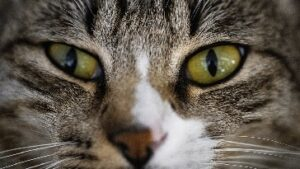
\includegraphics[scale=.5]{a20140814TheGreatCatPhotoContest-img001.jpg} 
\end{wrapfigure}

The visitors at the cat photo contest look for the cutest cat. However, the judges consider different factors such as originality, technical excellence, composition, artistic merit, and overall impact. The point is that the cat is irrelevant, since the same factors are used to judge every other photo contest. In other words, for the naïve visitors, the cat in the picture is the object of interest. However, for the judges, the photograph itself is the object of interest. The judges see through the photograph to the agent who created it.

Social analysis follows analogous rules. One can be like the cat lover and take what is going on as complete in itself. Then he will choose a position that he thinks is the cutest. The alternative is to understand events as a battle of worldviews and the hidden factors that propel them.

\paragraph{The Marketplace of Ideas}
John Stuart Mill was said to be remarkably intelligent, but the concept of a marketplace of ideas is ludicrous. Allegedly, in a free discussion the better ideas (or better, worldviews) will win out. But that assumes that the ideas in the marketplace are objective, fair, and disinterested. It leaves out of the equation those who create or promulgate certain worldviews and why they do it.

The worst people, who assume they are the most intelligent, are the ones who say things like “I will listen to both sides of the issue and then decide.” That makes them purely passive receptacles of others’ ideas. In a fair market, all parties are privy to all information. For example, if there is a drought in some coffee producing region, everyone knows it and the price takes that into account. That is why sellers try so hard to create unfair markets: e.g., by hiding information, locking competitors out, and trying to establish brand name distinctions.

So how fair is the marketplace of ideas? First of all, unlike news about coffee droughts which are less likely to be ideologically biased, the promulgation of ideas and worldviews is tightly regulated. In the USA, for example, six corporations account for nearly all the news sources. Many ideas, considered beyond the pale, are prohibited from the market place … there is no need to identify them. So the choice is quite limited.

Then there is the issue that in modern times, complex ideas require a deep knowledge of science, economics, mathematics, history, and philosophy to be fully understood. Now I know for a fact that such a breadth of knowledge is not very common.

At university, for example, I signed up for a logic class in the philosophy department. There were 25 students on day 1, but only three of us finished the course. Specifically, the future philosophers, journalists and political scientists all failed to take a formal course in logic. Economics was another class with a high dropout rate. You can probably assume that the talking heads on TV are woefully ignorant of economics. Forget science class altogether, because if you don't sign up, you won't have to drop out. Yet these commentators claim to understand difficult questions in climatology and human genetics.

Most amazingly is that everyone things himself capable of understanding issues of politics and metaphysics. Yet, to be admitted to Plato's Academy, it was first necessary to master maths before considering those issues, as we pointed out several years ago in Maths and Politics.

\paragraph{Development of Thought}
There are two ways to try to move human thought further: the revolutionary and the evolutionary.

\textit{Revolution:}
The revolutionary way is to take the dominant idea and proclaim its opposite. After a while, this gets very easy and predictable. It started with the reformation, enlightenment, and the French revolution. The reformation challenged the dominant spiritual authority, the enlightenment challenged the very idea of a spiritual authority, and finally the French revolution overthrew both the spiritual authority and the political power.

Karl Marx gave the revolutionary impetus a firm philosophical foundation. First of all, he correctly recognized that a “spectre”, or spirit, is haunting Europe. This is not a metaphor or other figure of speech as our cat lovers might suppose. The goal of that spirit is to overthrow the existing social and political order of things. Yet people I speak to who are haunted by that spectre never seem to recognize themselves as Marxists in spirit.

Subsequent developments in the West all follow from this. Marx was interested in the economic-political order, so he proposed that the proletariat would be the agents for the overthrow. However, developments a century later added some complexity. If the socio-political order is understood to be white dominated, then minority races become the new agents for the overthrow. If that order is understood to be male dominated, then women as feminists become the new agents. If that order is understood as hetero-normative, then deviant sexuality becomes the new agent.

With this principle, everything comes into focus. The revolutionary worldview is certainly original, it is promulgated with technical excellence through the mass media, and its overall impact is undeniable. Eventually the revolution itself becomes the established order and it is difficult to see where else it can go from there. Reaction won't automatically follow, since reaction is the opposite of the revolution.

\textit{Evolution:}
The evolutionary way is the way of depth. Previous thought is not overturned, but is understood on a deeper level. There are two ways to initiate that process:

\begin{itemize}
\item Bring out all the logical consequences of earlier thought 
\item Integrate it into a larger whole 
\end{itemize}
Here was need only recap what was written in more detail in recent weeks. From Tomberg to Keyserling, we see the method of depth described. The meaning of things is contemplated, even if it is multivocal. Freedom of the will is the foundation for thought and action.

\flrightit{Posted on 2014-08-14 by Cologero}

\begin{center}* * *\end{center}

\begin{footnotesize}\begin{sffamily}

\texttt{jc on 2014-08-21 at 06:28 said:} 

Lately I have been interested in the works of Kurt Gödel, amongst the realisation that we do live in a universe that is interconnected and infinitely more complex than we initially imagine.

It's only when we understand fundamentals like what was written about Plato's academy, that metaphysics takes on a deep and ontological meaning. There are no short cuts, though there are real and tangible gains.

\hfill

\end{sffamily}\end{footnotesize}


\end{document}
